 
%\documentclass[]{aa}
%\documentclass[draft]{aa}
%\documentclass[referee]{aa}

\usepackage[varg]{txfonts}

\usepackage{graphicx}

%\usepackage[x11names]{xcolor}
\usepackage{soul}

\usepackage{multirow}	%for tables

\newcommand{\Rs}{$R_\sun{}$}

\usepackage{siunitx}
	\DeclareSIUnit[number-unit-product=\,]\au{au}
	\DeclareSIUnit[number-unit-product=\,]\nT{\nano\tesla}
	\DeclareSIUnit[number-unit-product=\,]\Rs{\textit{R}_\sun{}}
	\sisetup{table-figures-uncertainty=2, table-number-alignment=center, range-phrase=--, range-units=single}



\documentclass[]{aa}
%\documentclass[draft]{aa}
%\documentclass[referee]{aa}

\usepackage[varg]{txfonts}

\usepackage{graphicx}

%\usepackage[x11names]{xcolor}
\usepackage{soul}

\usepackage{multirow}	%for tables

\newcommand{\Rs}{$R_\sun{}$}

\usepackage{siunitx}
	\DeclareSIUnit[number-unit-product=\,]\au{au}
	\DeclareSIUnit[number-unit-product=\,]\nT{\nano\tesla}
	\DeclareSIUnit[number-unit-product=\,]\Rs{\textit{R}_\sun{}}
	\sisetup{table-figures-uncertainty=2, table-number-alignment=center, range-phrase=--, range-units=single}




%AFFECTS
%Promotions-Thema:
%Original:
	%Analyse der Plasma- und Magnetfelddaten des ACE (Advanced Composition Explorer) -Satelliten zur Erstellung von "Echt-Zeit"-Weltraumwetterwarnungen und zur Modellierung solarer Einflüsse auf die terrestrische Ionosphäre im Rahmen des EU FP7 Projektes AFFECTS (Advanced Forecast For Ensuring Communications Through Space).
%Kürzer:
	%Analyse der Plasma- und Magnetfelddaten des ACE-Satelliten zur Erstellung von Echtzeit-Weltraumwetterwarnungen und zur Modellierung solarer Einflüsse auf die terrestrische Ionosphäre im Rahmen von AFFECTS.

	%Analyse von in-situ Sonnenwinddaten zur Erstellung von ``Echtzeit''-Weltraumwetterwarnungen und zur Modellierung solarer Einflüsse auf die terrestrische Ionosphäre.
	
	%Analyse von in-situ Plasma- und Magnetfeld-Sonnenwinddaten - Modellierung der Entwicklung des Sonnenwindes von der Sonne zur Erde und sein Einfluss auf das Erdmagnetfeld zur Erstellung von nahezu Echtzeit-Weltraumwetterwarnungen.

%Original translated:
	%Analysis of plasma and magnetic field data from the ACE (Advanced Composition Explorer) spacecraft for the generation of real-time space weather alerts and for the modeling of solar influences on the terrestrial ionosphere in the context of the EU FP7 project AFFECTS (Advanced Forecast For Communications Through Space).
%Short:
	%Analysis of plasma and magnetic field data from the ACE spacecraft for the generation of real-time space weather alerts and for the modeling of solar influences on the terrestrial ionosphere in the context of the EU FP7 project AFFECTS.

	%Analysis of plasma and magnetic field data from the ACE spacecraft, generation of real-time space weather alerts and modeling of solar influence on the terrestrial ionosphere.

	%Analysis of solar wind plasma and magnetic field in-situ data, generation of near real-time space weather alerts and modeling of the solar influence on the terrestrial magnetic field.
	
	%Analysis of solar wind plasma and magnetic field in-situ data - modeling of solar wind evolution from Sun to Earth and of its influence on the terrestrial magnetic field for the generation of near real-time space weather warnings.
%short:
	%Analysis of solar wind in-situ data - modeling of the solar wind evolution to Earth and of the influence on its magnetic field.
	%Modeling of the solar wind's evolution to Earth and of its influence on the terrestrial magnetic field by analysing solar wind in-situ data.
	

%daraus abgeleiteter Titel in Deutsch:
%Modellierung und Analyse solarer Einflüsse auf die terrestrische Ionosphäre/Magnetosphäre
%Translated titel (topic):
%Modeling and analysis of solar influences on the terrestrial ionosphere/magnetosphere




%daraus abgeleiteter Titel in Deutsch (Version 2):
%Analyse von in-situ Sonnenwind-Messungen zur Erstellung von Echtzeit-Weltraumwetterwarnungen und zur Modellierung solarer Einflüsse auf die terrestrische Ionosphäre...


%SolarProbePlus CGAUSS
%Theme has to be updated, because of SolarProbePlus work...
%Maybe: Analyses of solar wind influence on the terrestrial ionosphere/magnetosphere and modeling of solar wind within the near Sun region

%Analyse der Helios-Datensätze für die Modellierung des Sonnenwindes im Bereich des SolarProbePlus Orbits für die WISPR-Kamera


% maltes_commands.tex
% full journal name replacement
\def\aj{{Astron~.J.}}				%\def\aj{{AJ}}
\def\araa{{Ann~.Rev~.Astron~.Astrophys.}}	%\def\araa{{ARA\&A}}
\def\apj{{Astrophys~.J.}}			%\def\apj{{ApJ}}
\def\apjl{{Astrophys~.J.,~Lett.}}		%\def\apjl{{ApJ}}
\def\mnras{{Mon~.Not~.R~.Astron~.Soc.}}		%\def\mnras{{MNRAS}}
\def\aap{{Astron~.Astrophys.}}			%\def\aap{{A\&A}}
\def\nat{{Nature}}				%\def\nat{{Nat}}
\def\apjs{{Astrophys~.J.,~Suppl~.Ser.}}		%\def\apjs{{ApJS}}
\def\pasp{{Publ~.Astron~.Soc~.Pac.}}		%\def\pasp{{PASP}}

% other short commands
\def\ion#1#2{{\rm #1}{\sc #2}}
\newcommand{\Hi}{\ion{H}{i}}
\newcommand{\Hii}{\ion{H}{ii}}

% new since 2015
\def\planss{{Planet~.Space~Sci.}}		%Planetary and Space Science
\def\grl{{Geophys~.Res~.Lett.}}			%Geophysical Research Letters
\def\ssr{{Space~Sci~.Rev.}}			%Space Science Reviews
\def\jgr{{J~.Geophys~.Res.}}			%Journal of Geophysical Research

% new since 2016-10-20
\newcommand{\Rsun}{$R_\odot$}
\def\solphys{{Solar~Phys.}}			%\def\solphys{{SoPh}}	%Solar Physics
\def\aapr{{Astron~.Astrophys~.Rev.}}		%\def\aapr{{A\&ARv}}	%The Astronomy and Astrophysics Review

% new since 2017-10-05
\newcommand{\Kp}{\textit{Kp}}

% new since 2017-11-04
\def\zap{{Z~.Astrophys.}}			%\def\zap{{ZAp}}	%Zeitschrift für Astrophysik
\def\procspie{{Proc~.SPIE}}			%Proceedings of the SPIE

% aa compatibility
% 2017-11-04

\newcommand*{\sun}{\ensuremath{\odot}}
\newcommand{\Rs}{$R_\sun{}$}

\newcommand{\vBz}{$vB_\text{z}$}
%\renewcommand{\~}{\hbox{-}}	%replaces the command letter-tilde with nonbreaking hyphen


% abstract
\def\titley#1{{\chapter{#1}}}			%add 'y'
\def\subtitley#1{{#1\\}}				%add 'y'
\def\abstracty#1#2#3#4#5{{#1\\#2\\#3\\#4\\#5}}	%add 'y'
%\def\institute#1{{}}
%\def\keywords#1{{}}

% acknowledgments
\def\acknowledgements#1{\section{Acknowledgments} #1}


%tablefootnote taken from aa.cls:
\newlength{\VSpaceBeforeTabBib}
\setlength{\VSpaceBeforeTabBib}{2ex}
\newlength{\VSpaceBeforeTabFoot}
\setlength{\VSpaceBeforeTabFoot}{2ex}

\newcommand*\aa@tablefootname{Notes}
\newcommand*\aa@tablefootfont{\small}
\newcommand*\aa@tablefootnamefont{\small\bfseries}

\newcommand\tablefoot[1]{\VSpaceBeforeTabBib=1ex
  \par\vspace{\VSpaceBeforeTabFoot}
  \noindent
  \begin{minipage}{\linewidth}
    {\aa@tablefootnamefont\aa@tablefootname}~
    \aa@tablefootfont
    \ignorespaces
    #1
  \end{minipage}
}
\newcommand*\tablefootmark[1]{
  \unskip
  \hbox{\@textsuperscript{\normalfont\itshape\ignorespaces#1}}
  \,
  \ignorespaces
}
\newcommand\tablefoottext[2]{
  \hbox{\@textsuperscript{\normalfont({\itshape\ignorespaces#1})}}
%  ~
  \ignorespaces
  #2\ \ignorespaces
}


%search & replace for figures:
%[width=18cm] -> [width=\textwidth]

%\t\\resizebox\{\\hsize\}\{!\}\{\\includegraphics\{([^\}]*)\}\}\n\t
% to
%\t\\fcapside[\\FBwidth]\{\n\t\t\\includegraphics[width=0.5\\textwidth]\{\1\}\n\t\}\{\n\t\t

% \t\\label\{fig:([^\}]*)\}
% to
% \t\t\\label\{fig:\1\}\n\t\}





%\includeonly{filename1,filename2,...}

\begin{document}
	%\include{filename} essentially does a \clearpage before and after \input{filename}
	\pagenumbering{Roman}
	
\begin{titlepage}
	\begin{center}
	
	%formelle Titelseite und Rückseite übernehmen.?
	%Unilogo einfügen...
	
		\vspace*{10mm}
		\Large

		%\textbf{Analyses of solar-wind influence\\ \vspace{2mm} on the terrestrial iono-/magnetosphere\\ \vspace{2mm} and modeling of solar wind\\ \vspace{2mm} within the near Sun region}
%Analyses of solar-wind influence on the terrestrial ionosphere/magnetosphere and modeling of solar wind within the near Sun region
		%\textbf{Modeling of the solar wind's evolution to Earth\\ \vspace{2mm}and of its influence on the terrestrial magnetic field\\ \vspace{2mm}by analysing solar-wind in-situ data}
%Modeling of the solar wind's evolution to Earth and of its influence on the terrestrial magnetic field by analysing solar-wind in-situ data.
%		\textbf{Solar wind -- Variability, evolution to Earth\\and influence\\on the terrestrial magnetic field}
		\textbf{Solar wind -- influence on the magnetosphere\\and evolution to Earth} 
		
		\vspace{15mm}
		\large
		Doctoral thesis in physics\\
		\vspace{15mm}
		\textit{Malte~S.~Venzmer}\\
		%aus Stenum?
		\vspace{10mm}
		
		%make cover page image...
		
		\vspace{10mm}

		University of Göttingen\\
		\vspace{5mm}
		Institute for Astrophysics\\
		\vspace{5mm}
		January 2012 -- Jan? 2018\\
		\vspace{15mm}
		Supervisor:\\
		Dr.~Volker~Bothmer\\
		\vspace{5mm}
		Referees:\\
		Prof.~Dr.~Ansgar~Reiners\\
		Prof.~??\\
		
		
	\end{center}
\end{titlepage}

\newpage

\vspace*{5cm}

%Zitat in Diplomarbeit:
%\textit{"[...], und während er sich solchermaßen in der unteren Region des Reiches der Wissenschaft bewegte, dort, wo dieses unmerklich in das Reich der Psychiater übergeht, eignete er sich schließlich doch eine ganze Menge durchaus nützlicher Kenntnisse an, [...]"}
%denn er wusste immer erstaunlich gut Bescheid,
%\noindent Zitat: Stanislaw Lem, "Die Stimme des Herrn", S.56.

%quotes '"``''

\textit{``Despite the `Dr.' before his name, he had completed no course of study and received no degree. When people tried to pin him down about this, he would say that the letters were merely an abbreviation of his first name - Drummond - which he did not use. But it was as `Dr.' Sam Laserowitz that he appeared in a number of science-fiction magazines; he was also known, in the circles of the fans of that genre, as a lecturer, and spoke on `cosmic' themes at their many conferences and convention. Laserowitz's speciality was earthshaking discoveries, wich he happened upon two or three times a year. [...] We really have no idea what a multitude of con men and crackpots inhabit the domain that lies halfway between contemporary science and the insane asylum.''}\\

\noindent Excerpt from Stanis\l aw Lem 1968, \textit{His Master's Voice} \citep[p.~38]{Lem1984}.

%quote vs quotation vs excerpt


\vspace{1cm}

\begin{footnotesize}
\noindent version log:\\
1	2013-11-06\\
2	2013-11-07	inserted lem excerpt\\
3	2014-09-01	outlined introduction structure and appendix key words\\
4	2014-09-11	bibtex included, lem excerpt citet\\
5	2014-09-12	included italic titles in bibliography\\
6	2015-01-12	worked on introduction structure and included magnetic butterfly diagram\\
7	2015-05-04	first printout, small additions\\
8	2015-07-03	coupling functions, content structure\\
9	2015-09-09	Alfv\'en wave velocity formula\\
10	2015-09-10	Appendix physics: Alfv\'en and compressional MHD waves, plasma beta; citation sources Cranmer2005, Kivelson1995\\
11	2015-09-15	CGAUSS work overview; DQCS model figure\\
12	2015-09-16	magnetic energy density is the same as magnetic pressure, abbreviations\\
13	2015-09-30	empirical solar-wind model plots in analyses, figure label [Figure 4.2  Text]\\
14	2015-10-02	table column decimal alignment; set caption width\\
15	2015-10-05	table units; radial parameter (N, T) profiles in literature\\
16	2015-10-06	literature radial electron density models; log-normal distribution\\
17	2015-10-07	log-normal formulae\\
18	2015-10-08	log-normal fit\\
19	2015-10-09	shape fit parameter table; radial variance fitting\\
20	2015-10-14	variance fit values; log-normal citation Bronstein\\
21	2015-10-19	radial distribution width fitting; clarifying of solar-wind model formulae structure and naming variables\\
22	2015-10-20	log-normal distribution width factor changes the shape!\\
23	2015-10-23	log-normal distributions mu and sigma plot\\
24	2015-10-30	new sigmafit2 figures implemented; formulae adaption\\
25	2015-11-02	reason for use of log-normal function\\
26	2015-11-20	single log-normal shape fit; not chisquare - SSR; $R^2$ in appendix\\
27	2015-11-26	reduced SSR into tables; table column aligning\\
28	2015-12-02	smoothing SSR integration\\
29	2015-12-07	integrating structure remarks from printout\\
30	2015-12-09	splitting analyses chapter into two; browsing folders for usable things for thesis\\
31	2015-12-10	integrating citations and references\\
32	2015-12-16	integrating citations and references\\
33	2015-12-18	solar-wind structures list of Richardson\\
34	2016-02-02	sws distributions\\
35	2016-02-11	basics structure\\
36	2016-02-12	analyses questions\\
37	2016-02-15	analyses structure; in situ, near-Sun\\
38	2016-02-16	Kp index internal resolution\\
39	2016-02-17	Bartels1962; non-breaking hyphen shorthand implemented\\
40	2016-02-18	analysesI structure\\
41	2016-02-25	abstract\\
42	2016-02-26	english comma\\
43	2016-03-01	Bartels Kp origin paper, bibtex reference\\
44	2016-03-02	abstract\\
45	2016-03-03	Planck paper\\
46	2016-03-07	formation of stars\\
47	2016-03-08	formation of stars\\
48	2016-03-16	solar interior structure\\
49	2016-03-17	solar interior structure\\
50	2016-03-18	solar surface\\
51	2016-03-22	Astronomical Almanac citation\\
52	2016-03-23	solar core definition\\
53	2016-03-26	sunspots\\
54	2016-03-29	Sun interior figure\\
55	2016-03-30	solar composition\\
56	2016-03-31	Sun interior figure finished; chromosphere\\
57	2016-04-01	Sun atmosphere figure finished\\
58	2016-04-03	chromosphere, corona, CV\\
59	2016-04-07	CV\\
60	2016-04-08	CV; heliosphere\\
61	2016-04-09	corona; heliosphere\\
62	2016-04-11	heliosheath magnetic bubbles; Opher2011\\
63	2016-04-12	heliosphere; voyagers; Gurnett2013\\
64	2016-04-13	solar-wind effects, solar rotation\\
65	2016-04-14	analysesI sws structure draft plots\\
66	2016-04-15	analysesI concept work\\
67	2016-04-19	incorporate annotations from processed printout\\
68	2016-04-21	incorporate annotations from processed printout II\\
69	2016-04-22	incorporate annotations from processed printout III\\
69	2016-04-23	updated .bst file (for displaying arXiv id); implemented optional url displaying for electronic version; Kp year variations\\
70	2016-04-24	Kp frequency by month statistics and plot; Sun and Earth tilt plot\\
71	2016-04-25	solar cycle extrema dates literature\\
72	2016-04-27	Kp semi annual variation, Rangarajan1997\\
73	2016-05-01	Kp frequency by year\\
74	2016-05-04	Kp + SSN plot; ACE data errors/gaps; log-normal plot; differential rotation plot\\
75	2016-05-05	aggregate correlation coefficient tables, CME fraction plot\\
76	2016-05-06	overall sws fractions\\
77	2016-05-17	figure sw frequencies by year; restructured solar-wind distributions section; formal cover page\\
78	2016-05-20	Earth-Sun distance; JPL web interface\\
79	2016-05-31	GSM system\\
80	2016-06-10	Offline Anmerkungen einarbeiten\\
81	2016-06-12	LaTeX Earth symbol package\\
82	2016-06-13	numbers=noenddot\\
83	2016-06-14	references removed comma before ampersand; offline Anmerkungen einarbeiten; thesis\_raw version\\
84	2016-06-17	gnuplot figures and latex; latex document style options\\
85	2016-06-19	header implemented\\
86	2016-06-20	minor things; introduction\\
87	2016-06-23	solar tilt axis\\
88	2016-06-24	solar rotation\\
89	2016-07-12	magnetosphere temp figure; analyses: solar-wind model\\
90	2016-07-13	lognormal spelling\\
91	2016-07-14	constant mass flow rate\\
92	2016-07-18	line-up periods\\
93	2016-07-19	line-up periods table\\
94	2016-07-20	redone line-up analysis\\
95	2016-07-21	line-up tables\\
96	2016-07-22	line-up fit function plots; coefficient table\\
97	2016-07-22	line-up sw types and period plots; overview plot\\
98	2016-07-24	line-up averaging and justification\\
99	2016-07-29	line-up rework\\
100	2016-07-30	line-up structure\\
101	2016-07-31	line-up table\\
102	2016-08-02	line-up structure\\
103	2016-08-03	line-up fits and table\\
104	2016-08-04	insert offline comments\\
105	2016-08-15	literature radial sw functions\\
106	2016-08-18	work offline comments in\\
107	2016-08-19	work offline comments in\\
108	2016-08-28	analyses II rework structure\\
109	2016-08-31	analyses II rework structure\\
110	2016-09-01	analyses II rework figures\\
111	2016-09-02	analyses II rework structure\\
112	2016-09-03	Helios latitude dependency\\
113	2016-09-04	extrapolation model fit parameter table; Helios latitude dependence\\
114	2016-09-06	work in offline comments\\
115	2016-09-14	implement median and mean in composite fit table; create kile project for thesis; url and raw fork\\
116	2016-09-17	Ulysses polar plot; solar distance plots\\
117	2016-09-18	for solar distance and latitude -> 4-panel figures created and implemented; appendix figures\\
118	2016-09-20	latitude plots updated\\
119	2016-09-26	single lognormal fit figure\\
120	2016-09-27	minor tweaks in analyses II\\
121	2016-09-29	simple fit table errors; table style\\
122	2016-10-05	lognormal fit errors for tables\\
123	2016-10-10	line-up passing remarks from AP\\
124	2016-10-12	siunitx package incorporated\\
125	2017-01-04	package fancyhdr replaced with scrlayer-scrpage; offline comments for Basics + Data incorporated\\
126	2017-01-06	package floatrow included for figure side captions; some cites; magnetometer\\
127	2017-01-08	sun figure updates and new ion energy spectrum figure incorporated\\
128	2017-01-13	offline comments, new chapter order\\
129	2017-01-18	activated hyperref package; included autoref and eqref; adjusted link colors; header links\\
130	2017-02-02	offline commtents\\
131	2017-02-03	offline commtents II, eclipse image\\
132	2017-02-06	basics figures with floatrow; flow structure\\
133	2017-02-07	ion energy spectrum figure\\
134	2017-02-09	Helios mission ssn plot\\
135	2017-02-12	offline comments\\
136	2017-02-13	section number link to toc; offline comments\\
137	2017-02-14	eclipse and magbfly figure captions\\
138	2017-02-16	offline comments\\
139	2017-02-19	coronal heating and sw acceleration\\
140	2017-04-22	set up git repository\\
141	2017-04-23	incorporate offline comments\\
142	2017-04-26	bipolar region draft\\
143	2017-04-27	magnetic layer Ossendrijver2003\\
144	2017-06-29	magnetosphere figure drafts implemented\\
145	2017-07-16	streamlined content - including paper and chapter2\\
146	2017-07-22	streamlined duplicate content\\
147	2017-10-05	Kp index data\\
148	2017-10-28	geomagnetic indices; Kp index; Kp to ap table\\
149	2017-10-29	Kp index\\
150	2017-10-30	OMNI s/c coverage figure\\
151	2017-10-31	OMNI s/c coverage figure upgrade; data set timeline figure\\
152	2017-11-01	SSN prediction; omega-effect\\
153	2017-11-02	alpha-omega dynamo; magnetogram figure upgrade\\
154	2017-11-03	worked on figure permissions; alpha-omega-figure\\
155	2017-11-04	paperMVVB inserted; worked on compatibility\\
156	2017-11-12	paperMVVB: figure size, tablefoot, adjusted table width; included chapter2; ordered file implementing\\
157	2017-11-14	figure permission Babaszkiewicz1998\\
158	2017-11-15	poking around in image credits; solar activity cycle\\
159	2017-11-16	solar activity cycle; Zhao image permission\\
160	2017-11-17	Zhao copyright symbol included; solar-wind; commata and sentence wording\\
161	2017-11-22	notes from github paper folder\\
162	2017-11-23	Ulysses figure permission and caption; pdfpages package; paper included as is\\
163	2017-11-24	GUM reference; Helios data frequency figure\\
164	2017-11-25	intro to paper\\
165	2017-11-26	intro to paper\\
167	2017-11-27	Cranmer2005 fig1; Banaszkiewicz fig\\
168	2017-11-28	HCS and Parker spiral\\
169	2017-11-29	heliosheath; Cranmer2005 permission\\
170	2017-11-30	chapter2 updated\\
171	2017-12-06	upgraded: title, abstract, introduction, basics outline, notes to chapter2; worked in offline comments until HMF\\
172	2017-12-08	MBPs; Solar wind section structure\\
173	2017-12-10	solar wind basics, draft figs for CIR and CME\\
174	2017-12-11	draft figs for COR2 CME and ACE MC; solar wind history\\
175	2017-12-13	B-field improvement\\
176	2017-12-14	B-field improvement \#2\\
177	2017-12-15	B-field improvement \#3\\
178	2017-12-16	B-field angles plot\\
179	2017-12-17	B-field improvement \#4\\
180	2017-12-21	B-field: four plots upgraded\\
181	2017-12-31	B-field: worked offline comments in; included chapter2 update\\
182	2018-01-01	autoref names; solar wind properties; literature\\
183	2018-01-02	sw helium share; plasma beta; source surface; mass flux considerations\\
184	2018-01-04	sw considerations; fast/slow wind\\
185	2018-01-05	fig Hundhausen; fast slow sw\\
186	2018-01-08	fast slow sw\\
187	2018-01-09	slow sw sources\\
188	2018-01-10	slow sw; slow/fast cycle pattern\\
189	2018-01-11	Wang1990\\
190	2018-01-14	HCS and SIR\\
191	2018-01-15	HCS + CIR\\
192	2018-01-16	in-situ event plots\\
193	2018-01-17	in-situ CIR/HSS plot\\
194	2018-01-19	CME/MC plot; VB comments\\
195	2018-01-20	VB comments\\
\\
\ISOToday{} \thistime{} -- last save
\end{footnotesize}

\newpage

%\abstract
\begin{abstract}
\section*{Abstract}
This thesis analyzes how strong the solar wind and its internal structures impact the terrestrial magnetosphere and how the solar wind evolves on its way from the Sun.
%magnetosphere impact
In situ solar-wind measurements from the near-Earth OMNI data set are analyzed together with time series of the planetary geomagnetic disturbance indicator \Kp{}. Correlation functions are compiled with regard to nowcast the magnitude of the geomagnetic disturbances from solar-wind measurements and to forecast them from remotely observed streams and CMEs.
%solar activity
In situ data from the near-Earth OMNI data set and sunspot number data is used for deriving functional dependences with the state of the solar cycle for the solar-wind parameters magnetic field strength, proton velocity, density, and temperature.
%solar distance
Data from the Helios~1 and 2 missions is analyzed and empirical solar-wind distance dependencies for \SIrange{0.3}{1.0}{\au} are derived. Additionally, in view of the planned near-Sun spacecraft mission Parker~Solar~Probe (PSP), the solar-wind environment is estimated down to \num{<10}~solar radii.\\

catch from chapter abstracts...\\

%key words: solar wind; sun: corona; sun: heliosphere; Parker Solar Probe (PSP); magnetosphere; Kp index\\
%German title:\\
%german abstract: Kurzfassung\\
\end{abstract}

%\cleardoublepage
%\tableofcontents
{\let\cleardoublepage\clearpage\tableofcontents}	%open contents on left page
\label{toc}
%\listoffigures
%\listoftables

		%cover_formal
	\pagenumbering{arabic}
	
\chapter{Introduction}
\label{chap:introduction}

%Kurzer Text zur Motivation für diese Arbeit; wie es zum Thema kam und wie das Ziel erreicht wurde

Introductory text -> motivation\\
- \Kp{} impact analysis\\
- solar activity analysis\\
- distance analysis\\

% Questions this work asks:\\	%Fragestellungen ausformuliert
% 	How strong is the solar-wind influence on the terrestrial magnetosphere?\\
% 	How often occur certain solar-wind ranges?\\
% 	How strong do different structure types influence the terrestrial magnetosphere?\\
% forecast:\\
% 	How can the impact strength of the solar wind be forecasted? (VBz->Kp L1-Alerts)\\
% 	How can the impact strength of CMEs be forecasted (V->Kp correlation for CMEs)?\\
% 	(How can the impact field strength of CMEs be forecasted (V->B correlation for CMEs)?)\\

% 	How does the solar wind evolve on its way from the Sun?\\
% 	How do the different structures evolve on their way from the Sun?\\
% 	What are the properties of the solar wind near the Sun?\\
% 	(Where does the solar wind get accelerated?)\\
% 	(How does the solar wind get accelerated?)\\
% 	(How is this related to the coronal heating problem?)\\

thesis goal: finding more precise relationships between parameters/quantities for being able to make better forecasts\\

%Synopsis	% Outline (chapters and their content)
This thesis merges the solar-wind analyses of its impact on the magnetosphere, its variation with solar activity, and its evolution to Earth. This work is structured as follows. In \autoref{chap:basics} the fundamentals about the Sun, its activity, solar wind, and space weather are laid. The instruments and data are described in \autoref{chap:data}. The influences on the \Kp{}~index from solar activity, solar wind, its streams, and CMEs are analyzed in autoref{chap:chapter2}. In \autoref{chap:empirical_solar_wind_model_for_the_inner_heliosphere}, which includes the published paper on the same topic (\autoref{chap:solar_wind_predictions_for_the_parker_solar_probe_orbit}), an empirical solar-wind model for the inner heliosphere is developed and used to estimate the near-Sun solar-wind environment for the planned PSP mission. \autoref{chap:summary} summarizes the results and gives an outlook for further studies. Useful equations, constants, and abbreviations are located in the \autoref{chap:physics}, \ref{chap:math}, and \ref{chap:glossary}.


\chapter{Basics}
\label{chap:basics}
%COFI -- chapter outline and flow integration
This chapter sketches the basics for the analyses performed in this work. First, the Sun's origin, inner structure, atmosphere and heliosphere are described. Then, the Sun's dynamics with its differential rotation and magnetic field generation are outlined. Further, the solar activity cycle is described, including the meridional flow circulation, appearance of active regions, the surface magnetic field change, and sunspot cycles. The heliospheric magnetic field is pictured from its photospheric emergence in magnetic bright points and coronal superradial expansion, through the formation of the heliospheric current sheet and the Parker spiral to the heliosheath. The solar wind and its properties, the origin of slow and fast streams, stream interaction regions, and coronal mass ejections are described. Furthermore, the space weather, the solar influence on Earth, the magnetosphere, solar wind-magnetosphere coupling, and geomagnetic indices are portrayed.
%first the existing structures, second their dynamics, last their influence on humans/their technology (space weather)


\section{Solar composition}
\label{sec:solar_composition}

%%% universe
13.8~billion years ago the Big~Bang formed our universe. The energy density of our universe consists of \SI{69.1}{\percent} dark energy, \SI{25.9}{\percent} dark matter and \SI{4.9}{\percent} baryonic matter, according to calculations using the inflationary $\Lambda$CDM cosmology together with the latest CMB temperature measurements \citep{Planck2016}.
%see Planck2016 page 31 Table 4		age of universe
%see Planck2016 page 31 Table 4 and en.wikipedia.org/wiki/Lambda-CDM_model#Parameters
%energy density consists of
%dark energy $\Omega_\Lambda = 0.6911$,
%matter $\Omega_\text{m} = 0.3089$,
%dark matter $\Omega_\text{c} = 0.2589$ and
%baryonic matter $\Omega_\text{b} = 0.0486$
After a few minutes the primordial nucleosynthesis left the universe in a state where the baryonic matter was composed of \SI{75.33}{\percent}\footnote{Percentages by mass.} hydrogen, \SI{24.67}{\percent} helium and traces of deuterium, tritium and lithium \citep{Planck2016}.
%see Planck2016 page 47 Eq. 73

%%% star formation
Over the years this gas cooled down and gravitationally accreted into molecular clouds and formed stars. The first generations of stars (Population~III) fused this gas to heavier elements (metals) and supernovae distributed them into space as a foundation for the formation of new stars of low and high metallicity (Population~II and I). Likewise, supernovae of these stars constantly enriched the interstellar medium with metals. Now, the interstellar medium in the Milky~Way consists of about \SI{32}{\percent} helium and traces of other metals \citep{Danziger1970}.\\
%In 20XX the Voyager~? probe measured a density of about ...\SI{0}{\per\cm\cubed} right outside of the heliopause (cite?).\\

%%% solar interior
Our Sun, a metal-rich Population~I yellow dwarf star, emerged 4.6~billion years ago \citep{Bahcall1995} from an accretion disk, formed by a collapsing rotating cloud. The compression within its center resulted in high temperatures, which initiated the fusion of hydrogen to helium (primarily pp~chain reaction). The fusion reactions produce huge amounts of energy and heat the solar center to a temperature of 15.7~million~kelvins \citep{Christensen-Dalsgaard1996}. The generated energy is transported through the solar body to its surface and eventually into space.
The core region extends to about 0.25~solar radii (\Rsun), where the declining temperature becomes insufficient for fusion reactions. The energy transport is dominated by thermal radiation until, because of declining ionization and density, at 0.71\,\Rsun{} up to the surface convective motion takes over \citep{Christensen-Dalsgaard1991}. %0.7: http://adsabs.harvard.edu/abs/1991ApJ...378..413C
%Dalsgaard Model S: http://astro.phys.au.dk/~jcd/solar_models/
%core radius (cite?)

%%% photoshere + sunspots
The temperature at this transition region (tachocline) is about 2~million~kelvins and decreases up to the solar surface to between \SIrange{4400}{6600}{\K} (cite?). Here at the photosphere, the energy is radiated away with an effective black body temperature of \SI{5772}{\K} \citep{Mamajek2015}, classifying the Sun as a spectral type G2V star.
At this surface layer granules, the tops of convection cells, and temporary sunspots are visible. Strong magnetic flux inhibits the convection at sunspots, leading to lower temperature and brightness (for more details on sunspots see the next \autoref{sec:solar_dynamics}). \autoref{fig:sun_interior_HMIIC} illustrates these photospheric features along with the inner solar structure.\\
\begin{figure}[htb]
	%\centering
	\fcapside[\FBwidth]{
		\includegraphics[width=0.6\textwidth]{images/own_figures/sun_interior_HMIIC.png}
	}{
		\caption{Image of the photosphere together with a schema of the solar interior structure. The inset shows the granular surface with a sunspot. The figure is based on a SDO/HMI continuum image from 20~March~2016, credit: NASA/SDO and the AIA, EVE and HMI science teams.}
		\label{fig:sun_interior_HMIIC}
	}
\end{figure}

%%% chromosphere + corona + CMEs
Above the photosphere at the base of the chromosphere, the temperature declines to its solar minimum of \SI{3800}{\K} until it raises to \numrange{2}{3}~million~kelvins in the corona \citep{Billings1959,Liebenberg1975}. Up to now it is not fully understood why the corona is so much hotter than the underlying chromosphere -- this question is known as the coronal heating problem. The energy transfer mechanisms of choice are magnetic reconnections, wave heating and type~II spicules or a combination of these (cite?).

The chromosphere is a \SI{2000}{\km} thick region whose features (numerous spicules, filaments and prominences) can reach far into the corona. They consist of chromospheric material channeled by the solar magnetic field, which is enveloped by a thin transition region where the temperature jumps up from ?\SIrange{20000}{35000}{\K} to coronal temperatures (cite?). Reconnection of magnetic field lines can result in the eruption of filaments into the corona and beyond, termed coronal mass ejections (CMEs) (see also Section~XX...). Details of chromospheric features are shown in \autoref{fig:sun_atmosphere}.

%%% coronal holes
The Sun's atmosphere is dominated by the varying small- and large-scale solar magnetic field configuration. There are regions where the magnetic field lines arc back to the surface and regions with open field lines. In the latter areas the coronal plasma can -- guided by the field -- escape into space. Thus these coronal areas are less dense, cooler and therefore appear darker in extreme ultraviolet (EUV) and are called coronal holes (more in Section~XX...). In \autoref{fig:sun_atmosphere} a coronal hole is located at the solar south pole.
\begin{figure}[htb]
	%\centering
	\fcapside[\FBwidth]{
		\includegraphics[width=0.6\textwidth]{images/own_figures/sun_atmosphere.png}
	}{
		\caption{Composite image of the solar atmosphere and some of its features. Corona, chromosphere and photosphere are seen in wavelengths of \SI{193}{\angstrom}, \SI{304}{\angstrom} and continu\-um. Chromospheric spicules are visible on the northern limb. The enlargements on the right show a prominence and a filament. The dark region at the south pole is a coronal hole. The left inset shows details of the active region belonging to the sunspots in \autoref{fig:sun_interior_HMIIC}. The figure is based on SDO/AIA images from 20~March~2016, credit: NASA/SDO and the AIA, EVE and HMI science teams.}
		\label{fig:sun_atmosphere}
	}
\end{figure}

%%% corona
From Earth, the faint corona and chromosphere can only be observed during eclipses, because of the brightness of the solar disk. There are three effects contributing to the visibility of the corona: photon scattering off free electrons and dust particles, and ion spectral emission lines (termed K-, F- and E"~corona).
% the so-called K-, F- and E"~corona (K kontinuierlich, F Fraunhofer, E emission).\\
% K-corona: photon scattering off free electrons --> coronagraphs\\
% F-corona: photon scattering off dust particles; contains Fraunhofer absorption lines; expands in ecliptic as zodiacal light --> coronagraphs\\
% E-corona: ion spectral emission lines; reveals coronal composition --> images\\
The image of a solar eclipse reveals the coronal plasma, shaped by the magnetic field, and features of the red chromosphere, pictured in \autoref{fig:Tse2008_500_mo1}.\\
\begin{figure}[htb]
	%\centering
	\fcapside[\FBwidth]{
		\includegraphics[width=0.6\textwidth]{images/Tse2008_500_mo1.png}
	}{
		\caption{Total solar eclipse image of the inner corona up to 5~solar radii. The picture was taken in Mongolia, 1~August~2008 and is processed from multiple images. The magnetic field's dipole structure and the equatorial streamer belt, typical for a quiet Sun in cycle minimum, are visible. Credit: \href{http://www.zam.fme.vutbr.cz/~druck/Eclipse/}{Miloslav Druckmüller, Peter Aniol, Jan Sládeček}, 2008, reproduced with permission.}
		\label{fig:Tse2008_500_mo1}
	}
\end{figure}
%figure source: http://www.zam.fme.vutbr.cz/~druck/Eclipse/Ecl2008m/Tse2008_500_mo1/Hr/Tse2008_500_mo1.png

%%% solar-wind + heliosphere
Due to the high coronal temperatures, plasma escapes from the solar gravitational field \citep{Parker1958} with velocities of \SIrange{200}{800}{\km\per\s}. Its acceleration is linked to the coronal heating, however the exact location and process remain an open question (cite?). The magnetic field becomes too weak to guide the coronal plasma at a distance of a few solar radii. From this source surface, the solar wind flows radially outward into space until it reaches the termination shock. Eventually it collides with the local interstellar medium, creating the boundary of the heliosphere, the heliopause, which is expected to be a bubble of either teardrop or croissant shape (and may be led by a bow shock), caused by the Sun's relative velocity of \SI{23}{\km\per\s} to the local interstellar medium \citep{Owens2013, Opher2015}. Measurements of the Voyager~1 and 2 spacecraft indicate their passage of the termination shock at about \SI{94}{\au} and \SI{84}{\au}, entering the heliosheath region \citep{Owens2013}. \citet{Gurnett2013} report that in 2012 Voyager~1 actually crossed the heliopause into interstellar space at a solar distance of \SI{121}{\au}. \autoref{fig:Owens2013_Heliosphere_screenshot} illustrates the heliosphere and its surrounding flow structure.
\begin{figure}[htb]
	%\centering
	\fcapside[\FBwidth]{
		\includegraphics[width=0.6\textwidth]{images/Owens2013_Heliosphere_screenshot.png}
	}{
		\caption{Schema of the heliosphere and its surrounding flow structure. The heliosphere is formed by the interaction of the solar wind with the local interstellar medium at the heliopause. Credit: \citet[][Fig.~9]{Owens2013}, licensed under \href{https://creativecommons.org/licenses/by-nc/3.0/de/}{CC BY-NC 3.0 DE}.}
		\label{fig:Owens2013_Heliosphere_screenshot}
	}
\end{figure}
% contacted for permission...
%Owens2013 figure permission request: open access article

%%% solar-wind influence + space weather
On its way outwards through the solar system, the solar wind -- carrying the solar magnetic field -- interacts with the planets, their magnetic fields and other solar system bodies. These interactions have various effects, for instance disturbances in planetary magnetic fields with appearance of aurorae and enhanced radiation, atmospheric losses and stripping of cometary tails. Some of these effects can have disruptive consequences for humans and their technology. The topic of space weather effects is further addressed in \autoref{sec:space_weather}. The magnitude of these effects depends highly on spatial and temporal variations in the solar wind, which are rooted in the dynamics of the solar magnetic field.

%%%%%%%%%%%%%%%%%%%%%%%%%%%%%
%\section{Stars/Beginning}
% introduction leading to stars; beginning from universe/big bang\\
% gravitational contraction of rotating nebula\\
% -> fusion burning; energy production\\
% In its core it fuses hydrogen to helium; 15.7~million~K; inner 25~\%\\
% energy transport -> radiation zone; up to 70~\%\\
% tachocline ~2~million~K\\
% energy transport by convection -> convection zone; up to surface\\
% convective granulation\\
% photoshere 4400--6600~K, effective black body temperature 5777~K; spectral class\\
% (herzsprung russell diagram)\\
% chromosphere... (solar atmosphere figure)\\
% transition region\\
%corona 1--3~million~K temperature (coronal heating problem)\\
% coronal holes: open magnetic field lines, solar wind\\
% heliosphere, shock with interstellar medium (ISM); Voyager\\

%%%%%%%%%%%%%%%%%%%%%%%%%%%%%
%big bang
%to formation of stars
%to ISM in our galaxy
%to formation of Sun
%Sun's inner structure (energy production and transport)
%its surface (radiation, spectral class)
%its outer structure (chromosphere, corona, solar wind, heliosphere)
%its heliosphere (termination shock with ISM, Voyager measurements)
%%%%%%%%%%%%%%%%%%%%%%%%%%%%%


\section{Solar dynamics}
\label{sec:solar_dynamics}
%%% differential rotation + solar magnetic field origin
The spin conservation of the contracting molecular cloud led to a rotation of the Sun with a current average period of about 25~days. The radial convective motion within the solar interior above the tachocline leads to a transport of momentum away from the rotation axis and therefore to a slower polar and faster equatorial rotation in the convection zone \citep{Miesch2005}. This differential rotation is visible on the surface and was first discovered from sunspot observations. %in 1630 https://en.wikipedia.org/wiki/Solar_rotation
With a rotation period of about 34~days the poles have a lag of almost 9~days (for further information on solar rotation see appendix \autoref{sec:solar_surface_differential_rotation}). The differential rotation in the solar interior can be inferred from helioseismological observations, see \autoref{fig:Miesch2005_fig1a_interior_diff_rot}.
\begin{figure}[htb]
	\begin{floatrow}
		\ffigbox{	%[\FBwidth][]{
			\includegraphics[width=0.5\textwidth]{images/Miesch2005_fig1a_interior_diff_rot.png}
		}{
			\caption{Angular rotation velocity in the solar interior. The radiation zone has a nearly solid rotation. Above the tachocline (dashed line) begins the differential rotation of the convection zone. The angular velocity is inferred from helioseismology via observations from the Michelson Doppler Imager (MDI) at the Solar and Heliospheric Observatory (SOHO) spacecraft. Credit: \citet[][Fig.~3]{Thompson2003}, reproduced with permission, \textcopyright~Annual~Reviews.}
			%(\citet[Fig.~1\,a]{Miesch2005}; based on \citet[Fig.~3]{Thompson2003})
			\label{fig:Miesch2005_fig1a_interior_diff_rot}
			%Thompson2003 permission request: permission not required
		}
		\ffigbox{
			\includegraphics[width=0.28\textwidth]{images/Zhao2013_meridional_flow.png}
		}{
			\caption{Meridional flow velocity profile in part of the convection zone. Positive values are directed towards north. The velocity is inferred from helioseismology via observations from the Helioseismic Magnetic Imager (HMI) at the Solar Dynamics Observatory (SDO) spacecraft. Credit: \citet[][Fig.~4,\,panel~a]{Zhao2013}, reproduced with permission, \textcopyright~AAS.}
			\label{fig:Zhao2013_meridional_flow}
			%Zhao2013 permission request: permission granted.
		}
	\end{floatrow}
\end{figure}
%Angular velocity profile in the solar interior inferred from helioseismology (after Thompson et al., 2003). In panel (a), a 2D (latitude-radius) rotational inversion is shown based on the subtractive optimally localized averaging (SOLA) technique. All inversions are based on data from the Michelson Doppler Imager (MDI) instrument aboard the SOHO spacecraft, averaged over 144 days. Inversions become unreliable close to the rotation axis, represented by white areas in panel (a). Note also that global modes are only sensitive to the rotation component which is symmetric about the equator (courtesy M.J. Thompson \& J. Christensen-Dalsgaard).

%%% magnetic field dynamo mechanism
Turbulent plasma motions from convective flows in the convection zone generate and carry magnetic flux. The large rotational shear at the tachocline stretches and amplifies the disorganized magnetic fields ($\omega$-effect) to strong coherent toroidal flux with intensities of the order \SIrange{1}{10}{\tesla}. These toroidal fields, generated near the bottom of the convection zone, can be stored in a deep magnetic layer located in the stably stratified region below the convection zone \citep{Ossendrijver2003}. The stronger flux ropes become buoyant and raise to the surface. The Coriolis force twists them systematically, the twist is stronger at higher latitudes (Joy's law), on their way through the convection zone ($\alpha$-effect). They emerge then on the photosphere as bipolar active regions -- the stronger ones forming pairs of sunspots, see \autoref{fig:bipolar_region_HMIB_HMIIF}.
\begin{figure}[htb]
	\centering
	\includegraphics[width=\textwidth]{images/own_figures/bipolar_region_HMIB_HMIIF.png}
	\caption{Continuum image of both sunspots from \autoref{fig:sun_interior_HMIIC}, magnetogram from the same region and from the whole solar disk. The magnetogram shows the polarity of the line-of-sight magnetic field component at the photosphere (black/white: inward/outward polarity). The highly concentrated magnetic flux at the sunspots is clearly visible in the magnetogram as well as the extended bipolar magnetic field structure of the whole active region. The solar disk is scaled to the same size as in \autoref{fig:sun_interior_HMIIC}. The figure is based on SDO/HMI continuum and magnetogram images from 20~March~2016, credit: NASA/SDO and the AIA, EVE and HMI science teams.}
	\label{fig:bipolar_region_HMIB_HMIIF}
\end{figure}
% HMI is a vector magnetogram, but the public sources say that the magnetogram shows a line-of-sight magnetic field.
Turbulent convective diffusion of this surface flux contributes to the build-up of poloidal fields. Their resulting polarity is opposite to the prevailing global field, due to the directional way the rotational shear at the tachocline and the Coriolis force in the convection zone act. Fluctuating motions further amplify the mean fields in these processes. This solar $\alpha$-$\omega$-dynamo is thought to create the major part of the solar magnetic field. Still, with regard to the magnetic field's high variability, the long-term mean fields are governed by intermittent localized structures, that is, active regions, filaments and coronal loops \citep{Miesch2005}.	%Miesch2005 p.~18 + p.~31

the $\alpha$-$\omega$-dynamo, see \autoref{fig:EOSFIG2_modified}\\
\begin{figure}[htb]
	%\centering
	\fcapside[\FBwidth]{
		\includegraphics[width=0.5\textwidth]{images/EOSFIG2_modified.png}
	}{
		\caption{Schemata of the $\omega$ and the $\alpha$-effects. figure really necessary? get permission...}
		\label{fig:EOSFIG2_modified}
	}
\end{figure}
%http://certificate.ulo.ucl.ac.uk/modules/year_one/NASA_MSFC/solar_physics/dynamo.htm
%https://solarscience.msfc.nasa.gov/images/EOSFIG2.GIF

% switching between states of strong poloidal and toroidal field\\
% poloidal field + diff. rot. => toroidal field ($\Omega$-effect)\\
% the solar dynamo: (toroidal to poloidal field)\\
% - turbulent plasma motions from convective flows generate disorganized magnetic fields\\
% - differential shear at tachocline amplifies fields to strong coherent toroidal flux ($\Omega$-effect); magnetic layer located at the base of the convection zone\\
% - stronger flux ropes raise to surface (buoyantly)\\
% - Coriolis force twists them systematically, stronger at higher latitudes\\
% - twisted tubes emerge on the surface as bipolar active regions\\
% - amplification of mean fields by fluctuating motions ($\alpha$-effect) and turbulent diffusion create large-scale poloidal field\\


\section{Solar activity cycle}
\label{sec:solar_activity_cycle}
%%% convection cycle + solar surface magnetic field + solar cycle
Helioseismic measurements reveal that the large-scale convective flow is agglomerated into large convection cells with slow meridional flows of a few \si{\m\per\s}, see \autoref{fig:Zhao2013_meridional_flow}. A poleward subsurface flow and equatorward backflow beneath with a further poleward flow below are detected within each hemisphere, comprising a stacked double-cell profile. The meridional circulation flow speed has a major influence on the average 22-year period of the emerging magnetic flux at the solar surface. This period varies and is influenced by the stochastic emergence rate and tilts of active regions and the diffusion from random convective motions \citep{Hathaway2016}. Within one period, the surface magnetic field configuration changes from a dipole structure to a reversed dipole structure with opposite polarity, thus the transition time from one dipole state to the next lasts about 11~years, this period is termed solar cycle.
%http://www.solarcyclescience.com/forum/viewforum.php?f=9

%%% butterfly pattern
In the transition phase, magnetic flux emerges in belts above and below the solar equator, manifesting as bipolar active regions with sunspots, resulting in a toroidal/multipolar structured magnetic field. Sunspots appear at about \SI{+-20}{\degree} latitude at the beginning of a cycle, this shifts towards lower latitudes at the end of a cycle. Thus the plot of sunspots over latitude and time reveals a butterfly pattern \citep{Maunder1904}. This butterfly pattern appears in surface radial magnetic field observations as well, see \autoref{fig:Hathaway_magbfly}.
\begin{figure}[htb]
	\centering
	\includegraphics[width=\textwidth]{images/Hathaway_magbfly_201610.jpg}
	\caption{Magnetic butterfly diagram of the synoptic radial magnetic field on the solar surface. Yellow represents an outward directed magnetic field (positive), blue inward (negative). The data is obtained from instruments on Kitt~Peak National Observatory and from the MDI at the SOHO spacecraft. Credit: David~Hathaway, NASA Marshall Space Flight Center \citep[updated version of][Fig.~17]{Hathaway2015}. Update this figure before printing!}
	\label{fig:Hathaway_magbfly}
\end{figure}
%Hathaway 2015 permission request: open access article
%figure source:	http://solarscience.msfc.nasa.gov/images/magbfly.jpg
The leading polarity of bipolar regions is opposite in both hemispheres and the leading polarity changes with each cycle (Hale's polarity law). The emerging flux is carried by the slow meridional surface flow poleward, canceling the current dominating polar field polarity and eventually resulting in the polar field switch \citep{Hathaway2015}.

%%% sunspot number
Since regions of strong magnetic flux are visible as sunspots on the photosphere, they were known well before the common era by greek and chinese scholars \citep{Vaquero2007,Clark1978}. %greek sunspot observation: http://adsabs.harvard.edu/abs/2007JBAA..117..346V
Systematic sunspot observations exist since 1610, shortly after the invention of the telescope. In 1843 Schwabe discovered the 11-year periodicity in the sunspot occurence \citep[p.~124]{Schroeder2004}. In 1848 Wolf introduced the sunspot number (SSN), see \autoref{fig:ROB_ssn_wolfmms}, and the solar cycle number (the zeroth in 1749) to record these cycles \citep{Hathaway2015}.
\begin{figure}[htb]
	\fcapside[\FBwidth]{
		\includegraphics[width=0.6\textwidth]{images/ROB_ssn_wolfmms.png}
	}{
		\caption{Monthly mean sunspot number (blue) and 13-month smoothed monthly sunspot number (red) since 1954. Credit: \href{http://sidc.be/silso/monthlyssnplot}{SILSO data/image, Royal Observatory of Belgium, Brussels}, 2017. Update this figure before printing!!!}
		\label{fig:ROB_ssn_wolfmms}
	}
\end{figure}
%SIDC/SILSO permission request: permission not required
%image from:	http://sidc.be/silso/
The SSN observations show large variations in cycle length (9--14~years) and cycle amplitude, with peak SSNs in the range 0--300, \citep{Hathaway2015}. There also exist long-term variations, such as the 70"~year Maunder~Minimum, during which from 1645 on almost no sunspots were observed, \citep{Maunder1890}. The source of the variations in the solar cycle periods and amplitudes are variations in the meridional circulation, because their fluctuations are larger than those found in the differential rotation and in the convective motions \citep{Hathaway2015}.

%%% SSN prediction
As the SSN is commonly used as an indicator for solar activity, there exists interest in its prediction for the course of the actual and upcoming solar cycles. The continuing prediction of an already commenced activity cycle is reliable, but then the prediction of a cycle before it began is more difficult. Though, there are indications that the polar magnetic field strength during the preceding activity minimum is correlated to the strenght of the next solar cycle \citep{Schatten1987}. However, \citet{Hathaway2016} suggest that the predictability of solar cycles is generally limited -- accumulated uncertainty produced by stochastic motions in the convection zone makes predicitons further than the next solar cycle very unreliable.


\section{Heliospheric magnetic field}
\label{sec:heliospheric_magnetic_field}
%%% MBPs to canopy
In the quiet Sun during solar cycle minimum, open coronal regions are the photospheric sources of the heliospheric magnetic field (HMF). Bright points between the granules on the photosphere are detected in G-band (\SI{430}{\nano\meter}) images. They are identified as magnetic flux tubes with field strenghts of \SIrange{100}{200}{\milli\tesla} \citep{Cranmer2005}. Together these magnetic bright points (MBPs) cover around \SIrange{1}{2}{\%} of the solar surface and carry many times the flux that active regions do \citep{Sanchez_Almeida2010}. These thin flux tubes expand laterally in the low chromosphere and merge to homogeneous network fields, which expand and merge again to a large-scale canopy below the transition region (see \autoref{fig:Cranmer2005_fig1_ab}).
\begin{figure}[htb]
	\fcapside[\FBwidth]{
		\includegraphics[width=0.6\textwidth]{images/Cranmer2005_fig1_ab.png}
	}{
		\caption{Schemata of superradially expanding magnetic flux. MBPs between granules on the photosphere are thin magnetic flux tubes that merge to a homogeneous network field (a). The network field expands again to the large-scale canopy field of the lower corona (b). Credit: \citet[][Fig.~1]{Cranmer2005}, reproduced with permission, \textcopyright~AAS.}
		\label{fig:Cranmer2005_fig1_ab}
	}
\end{figure}

%%% Alfvén waves
The MBP's convective appearance and stochastic motions result in wavelike fluctuations that propagate upward from the photosphere through the superradially expanding flux tube -- leading to incompressible waves leaking into the solar wind \citep{Cranmer2005}. These Alfvén waves propagate with a characteristic speed along the magnetic field lines -- for more details about Alfvén waves and Alfvén speed see appendix \autoref{sec:alfvén_waves}. The local Alfvén speed equals the solar wind speed at around \SI{17}{\Rs} \citep{Sittler1999,Exarhos2000}. It is believed that the solar wind is accelerated until this so-called Alfvén critical surface (cite?).\\

%%% field geometry from source surface on to heliopause
The coronal plasma expands superradially, following the magnetic field lines. However, the field strength decreases with increasing solar distance and at a distance of about \SI{2.5}{\Rs} the thermal pressure becomes larger than the magnetic pressure. Thereby the magnetic field gets frozen within the plasma and is carried by the solar wind radially outwards into the heliosphere. The distance from which the solar wind propagation uncouples from the magnetic field lines is called the source surface \citep{Schatten1969} and the thermal to magnetic pressure ratio is called plasma beta -- for more details see appendix \autoref{sec:plasma_beta}. The magnetic field changes from superradial expansion below the source surface to a radial configuration above it, this field geometry is also visible in the total eclipse image \autoref{fig:Tse2008_500_mo1}.

%%% HCS
Under solar cycle minimum conditions, a heliospheric current sheet (HCS) separates the two different magnetic polarities originating from both polar coronal holes. The HCS is roughly located in the equatorial plane, dividing both hemispheres. The analytical solar magnetic field model for solar minimum conditions, constructed by \citet{Banaszkiewicz1998}, shows this field geometry as seen in \autoref{fig:Banaszkiewicz1998_DQCS_model_raw}. The quadrupole part of their dipole plus quadrupole plus current sheet (DQCS) model considers the closed equatorial fields and allows equatorial outflows along the current sheet.
\begin{figure}[htb]
	\begin{floatrow}
		\ffigbox{
			\includegraphics[width=0.45\textwidth]{images/Banaszkiewicz1998_DQCS_model_raw.png}
		}{
			\caption{Model of the solar magnetic field geometry in the polar plane for solar cycle minimum. Magnetic field lines (solid) and constant field strength surfaces (dashed) from the DQCS model are plotted. The field line spacing does not represent the field strength but provides better detail where needed. The HCS forms a few solar radii distance at $z = 0$. Credit: \citet[][Fig.~3]{Banaszkiewicz1998}, reproduced with permission, \textcopyright~ESO.}
			\label{fig:Banaszkiewicz1998_DQCS_model_raw}
		}
		\ffigbox{
			\includegraphics[width=\Xhsize]{images/Owens2013_PFSS_Sectors_screenshot.png}
		}{
			\caption{Illustration of the Parker spiral formation in the ecliptic plane outside the source surface. The HCS (green) forms between solar-wind flows of opposite magnetic field polarity (red/blue). Credit: \citet[Fig.~1]{Owens2013}, adapted from \citet[Fig.~1]{Schatten1969}, licensed under \href{https://creativecommons.org/licenses/by-nc/3.0/de/}{CC BY-NC 3.0 DE}.}
			\label{fig:Owens2013_PFSS_Sectors_screenshot}
			%Owens2013 figure permission request: open access article
		}
	\end{floatrow}
\end{figure}

%%% Parker spiral
The solar-wind source surface rotates with the Sun and thus shears the HMF into an Archimedean spiral pattern, adding an azimuthal component to the radial HMF. This geometry was anticipated by \citet{Parker1958} and is today called Parker spiral. Commonly the HCS looks more like a ballerina skirt, due to magnetic field variations, and thus the Parker spiral has sectors of different magnetic polarity, whose boundaries are separated by the HCSs. \autoref{fig:Owens2013_PFSS_Sectors_screenshot} shows the Parker spiral viewed in the ecliptic plane, where the solar rotation axis tilt of up to \SI{7.25}{\degree} leads to a slight diving into both hemispheres of opposite polarity.

%%% out to heliopause
That way the HMF is carried out to the termination shock by the solar wind. MHD simulations, based on Voyager~1 and 2 measurements within the heliosheath, provide indications about the outer structure of the heliosheath. After the termination shock, the magnetic sector boundaries are compressed and they reconnect, forming magnetic bubbles \citep{Opher2011}. These bubbles -- unconnected to the HMF -- flow away to the heliosheath tail region. Even beyond the termination shock, the solar wind plasma is confined and collimated by the twisted solar magnetic field and driven into a northern and a southern jet \citep{Opher2015}. Hence, the Sun's magnetosphere has likely a croissant-like shape with two turbulent tail-lobes, where eventually the solar wind and the HMF are mixed into the interstellar medium.


\section{Solar wind}
\label{sec:solar_wind}
%%% sw history
It is observed that cometary tails lag a few degrees from the radial direction away from the Sun, sometimes they also show fluctuations and become kinked. As such behavior could not be explained by interaction with sunlight pressure, eventually \citet{Biermann1951} concluded that cometary ion tails are influenced by a continuous flow of particles from the Sun.	%Kivelson1995, p14+91
\citet{Parker1958} considered the consequences of Biermann's conclusions and built a solar-wind model, adopting an expanding isothermal solar atmosphere. Parker also incorporated the implications for the solar magnetic field in his model and hence he laid the theoretical foundations for a continuous supersonic radial outflow of magnetized plasma. Thus, the existence of the solar wind was postulated before the first satellites measured it in~situ in 1959 \citep{Gringauz1960,Neugebauer1966}. Since that time, spacecraft are able to measure the solar wind almost continuously with in~situ magnetometer and plasma instruments (see \autoref{sec:instruments}). Pronounced solar-wind structures, such as CMEs and streamers, become visible with the use of space-based coronagraph imagers. From Earth, the outflow of near-Sun solar wind can also be observed during solar eclipses, see the eclipse photo in \autoref{fig:Tse2008_500_mo1}.

%%% plasma composition, parameter ranges and properties
The solar wind is a magnetized plasma consisting of electrons and ions. The ions are mainly composed of hydrogen, a small percentage of helium, and traces of oxygen, carbon, and other metals. The average abundance of helium (alphas) is about \SI{4.5}{\%} and in slow wind at solar cycle minimum conditions less than \SI{2}{\%} \citep{Feldman1978,Schwenn1983,Kasper2012}.
The solar wind is commonly approximated by an ideal incompressible magnetohydrodynamic plasma (viscosity $\mu = 0$ and electrical conductivity $\sigma = \infty$) and can be viewed as a neutral plasma. Also, its helium share is often viewed as being constant, in this case the proton density determines both the helium and electron densities. This work adopts these assumptions and treats the solar wind throughout as a proton plasma.

The properties of solar wind are highly variable in time and space. The properties are determined by the values of the solar-wind parameters magnetic field strength, proton velocity, density, and temperature. Their average magnitudes scale with solar activity, heliographic latitude, and solar distance. At a solar distance of Earth however, most of the time the parameter's typical values lie in the ranges \SIrange{3}{8}{\nano\tesla}, \SIrange{300}{500}{\km\per\s}, \SIrange{2}{8}{\per\cm\cubed}, and \SIrange{e4}{e5}{\K} (\citet[p.~92]{Kivelson1995}; \citet{Venzmer2017}). The low density of solar wind can be illustrated with a short comparison: 1~liter of air at standard pressure, expanded to a typical solar wind density of \SI{6.5}{\per\cm\cubed}, would occupy a volume of a cube with edge length of about \SI{155}{\km}.
% sw density considerations:\\
% 1 mol approx 24.7895 l/mol at 25 °C and 1 bar
% Avogadro constant N_A = 6.022140857(74)e23 mol−1
% 1 liter air @ 1 bar equates to 1/24.7895 mol = 2.4293e+22
% 2.4293e+22 / 6.5 cm-3 = 3.7374e+21 cm3 = 3.7374e6 km3 = (155 km)3
% 1 liter air @ 1 bar (need 24 ms for passing 1 dm2 area @ 15 km/h)\\
% equals\\
% 3.7e6 km3 = (155 km)3 solar wind @ 6.5 cm-3 (need 43900 a for passing 1 dm2 area @ 400 km/s)\\
Solar-wind quantities, such as particle flux densities, mass flux and plasma beta can be derived from the four listed parameters. Having the parameters in the aforementioned ranges, the solar wind is a plasma with a beta mostly greater than unity (for more on plasma beta see appendix \ref{sec:plasma_beta}).
% mean beta: 1.714\\	%from mean paper values
% low beta: 0.180\\	%from ranges above
% high beta: 8.444\\	%from ranges above

The solar wind is structured by its different sources in the solar corona. It consists of continuous streams and CME events. Their highly variable velocities result in compressed or rarefied regions at their interfaces. The solar wind is further structured by the magnetic field, which the plasma carries from its source region. Changes in its field direction and embedded magnetic structures have an influence on the plasma.\\


prepare following subsections:\\
slow/fast wind\\
-> following event/structure types\\
special events/configurations, which can appear (CIRs, HCS/HPS, etc.)\\
HSS, sector boundaries, CIRs, CMEs\\

prepare next subsection:\\
different source regions: sunspots/active regions, coronal holes, and filaments.\\


SEPs, neutral atoms...\\

MHD waves (Alfvén waves)\\
in HSSs (cite?)\\
Alfvén speed ca. 40~km/s (Kivelson1995)\\

sonic and Alfvénic critical point positions (see Sittler \& Guhathakurta (1999))\\
sonic point and slow solar wind origin (Sheeley et al. 1997)\\


\subsection{Slow and fast streams}
%%% fast and slow solar wind
It is observed that the continuous solar wind comes in streams roughly focused at two major velocity ranges \citep{Neugebauer1966,Schwenn1983}, slow and fast streams with \SIrange{250}{450}{\km\per\s} and \SIrange{450}{800}{\km\per\s} respectively. Both types possess differences in their typical characteristics and ion compositions. Apart from its higher speeds, fast solar wind has most prominently lower proton densities ($\sim$~\SI{3}{\per\cm\cubed}) and higher temperatures ($\sim$~\SI{2e5}{\K}) than the slow solar wind, which has higher densities ($\sim$~\SI{10}{\per\cm\cubed}) and lower temperatures ($\sim$~\SI{4e4}{\K}) \citep{Schwenn1990}. The fast solar wind has a nature of coming in steady high-speed streams (HSS) with a unique magnetic field polarity, whereas slow solar wind is much more variable in all its properties.\\

%sources of fast wind
First soft X-ray observations of the corona, made during sounding rocket flights, showed that the fast solar wind emerges from extended areas of reduced X-ray emission, subsequently called coronal holes (CHs) \citep{Krieger1973,Hundhausen1977}. The magnetic field polarities found in CHs are associated with the magnetic field directions observed in HSSs, see \autoref{fig:Hundhausen1977_fig10}.\\
\begin{figure}[htb]
	\fcapside[\FBwidth]{
		\includegraphics[width=0.5\textwidth]{images/Hundhausen1977_fig10.png}
	}{
		\caption{Solar-wind velocity with respect to its estimated source longitude (top) and coronal brightness contour map at \SI{0.5}{\Rs} above the photosphere (bottom) for the Carrington rotation 1616. The velocity is based on IMP spacecraft data, back-extrapolated to \SI{20}{\Rs}. Brightness values below a fixed threshold are shaded ($+$/$-$) corresponding to the magnetic field polarity of the underlying photosphere. The map is based on observations from the K-coronameter at the Manua~Loa Observatory. Credit: \citet[Fig.~10]{Hundhausen1977}, get permission...}
		\label{fig:Hundhausen1977_fig10}
	}
\end{figure}

sector boundaries...\\

In coronal regions with closed magnetic field lines the plasma is trapped, though in CHs it can escape following the open magnetic field lines outwards into space, forming into HSSs.\\
% fast wind emerges from CHs\\


%sources of slow solar wind
different types of slow solar wind \citep{Schwenn1983}\\

It is found to be difficult to trace the slow solar wind types to different origins and distinguish between them, because most parameters are highly variable in time \citep{Kilpua2016}. However, some indicators show tendencies to differentiate between the solar wind from different source regions. Notable indicators are elemental ion ratios, heavy ion charge states, and the specific entropy.\\

The elemental composition of the plasma varies with height in the solar atmosphere, therefore the elemental ion ratios (e.g., $\text{He}/\text{H}$, $\text{Fe}/\text{O}$) can determine its origin.\\

The charge states of heavy ions depend on the local coronal temperatures\\
the states freeze in very close to the Sun\\

heavy ion charge states (e.g., $\text{C}^{+6}\!/\text{C}^{+4}$, $\text{O}^{+7}\!/\text{O}^{+6}$)\\

carbon charge states are good indicators of the coronal temperature and in particular the $\text{C}^{+6}\!/\text{C}^{+4}$ ratio is sensitive to the solar wind type \citep{Landi2012}.\\


the specific entropy\\


tracing slow solar wind sources with\\

different sources for the solar wind are discussed:\\
- closed field/helmet streamers from loop cusps, magnetic sector boundaries, superradial expansion, \\
- quiet Sun wind -- slowest and coldest wind, with the lowest values of specific entropy\\
- active region wind -- HCS, streamer cusps\\
- CH wind -- CH boundary\\

sources of slow solar wind (Wang2000):\\
- slow CMEs\\
- small CHs\\
- CH boundaries\\
- streamer material (blobs)\\


origin from closed magnetic structures in the solar corona, such as intermittent reconnection at the top of helmet streamers and from coronal hole boundaries \citep{Kilpua2016}\\

The origin of slow wind is still under debate.\\


the overlapping ranges of the slow and fast solar wind \citep{McGregor2011a}\\

Superradial expansion has an influence on the wind speed, however, there are indications that the slow and fast solar wind are not only generated at different sources but from distinct mechanisms \citep{McGregor2011b}.\\



%solar activity dependence
The ordered dipole structure during solar cycle minima leads to open polar field regions with large coronal holes and a large equatorial belt region with closed magnetic fields -- this state is clearly visible in Figures~\ref{fig:Tse2008_500_mo1} and \ref{fig:Banaszkiewicz1998_DQCS_model_raw}.\\

sw in minimum: streamer belt and polar HSSs\\
minimum: polar coronal holes\\
active regions forming equatorial streamer belt\\
only fast solar wind at higher latitudes\\

cycle maximum:\\
This leads to the chaotic appearance of closed field lines even at higher latitudes/poles and coronal holes covering equatorial regions.\\

This is confirmed by the Ulysses spacecraft, which measured the solar-wind speed in a polar orbit covering more than one solar cycle (\autoref{fig:McComas2008_Ulysses_orbit}).\\
\begin{figure}[htb]
	\centering
	\includegraphics[width=\textwidth]{images/McComas2008_Ulysses_orbit_.png}
	\caption{Solar-wind velocity and magnetic field polarity (red/blue) with respect to heliographic latitude for the three orbits of the Ulysses spacecraft during low and high solar activity (upper panels). The data starts left and couterclockwise. The corresponding smoothed SSN (black) and HCS tilt angle (red) are plotted beneath. The background consists of solar images for solar cycle~22 minimum (1996-08-17), solar cycle~23 maximum (2000-07-12), and solar cycle~23 minimum (2006-03-28). The solar disk, inner corona, and outer corona images are from SOHO/EIT (Fe~XII at \SI{1950}{\nano\meter}), Mauna~Loa K~coronameter (\SIrange{700}{950}{\nano\meter}), and SOHO/C2 white light coronagraph. Credit: \citet[][Fig.~1]{McComas200809}, reproduced with permission, \textcopyright~American Geophysical Union. ...ask for high res. image?}
	\label{fig:McComas2008_Ulysses_orbit}
\end{figure}
%figure source: http://onlinelibrary.wiley.com/doi/10.1029/2003GL017136/full
%McComas200809: (a–c) Polar plots of the solar-wind speed, colored by IMF polarity for Ulysses' three polar orbits colored to indicate measured magnetic polarity. In each, the earliest times are on the left (nine o'clock position) and progress around counterclockwise. (d) Contemporaneous values for the smoothed sunspot number (black) and heliospheric current sheet tilt (red), lined up to match Figures 1a–1c. In Figures 1a–1c, the solar-wind speed is plotted over characteristic solar images for solar minimum for cycle 22 (8/17/96), solar maximum for cycle 23 (12/07/00), and solar minimum for cycle 23 (03/28/06). From the center out, we blend images from the Solar and Heliospheric Observatory (SOHO) Extreme ultraviolet Imaging Telescope (Fe XII at 1950 nm), the Mauna Loa K coronameter (700–950 nm), and the SOHO C2 white light coronagraph.

% paper:\\
% ``Fast streams are found to originate from coronal holes as confirmed by Ulysses' out-of-ecliptic measurements \citep{McComas1998}. The occurrence frequency of these slow and fast streams varies strongly with solar activity and their interactions lead to phenomena such as stream interaction regions which may persist for many solar rotations ("co-rotating" interaction regions) if the coronal source regions are quasi-stationary \citep{Balogh1999}.''\\



\subsection{Stream interaction regions}
%%% SIRs/CIRs and HCS/HPS
in-situ measurements (example in situ CIR/HSS plot)\\
stream interfaces (figure and link to previous CIR plot) -> HCS/HPS\\
equatorial ballerina model -> CIRs (figure?)\\

reviews: \citet{Balogh2009} (for heliosheath), \citet{Owens2013}\\

heliospheric current sheet (HCS)\\
heliospheric plasma sheet (HPS)\\

Winterhalter1994 The heliospheric plasma sheet:\\
"the narrow heliospheric current sheet (ca. \SIrange{3000}{10000}{\km} thick), together with the heliospheric plasma sheet in which it is embedded. The heliospheric plasma sheet region is identified by a significantly enhanced plasma beta caused by density enhancements and diminished magnetic field strength and is about 20 to 30 times the thickness of the current sheet."\\

``Low He/H values are in particular reported near solar wind sector boundaries.'' (Borrini et al., 1981)\\
The particularly low specific entropy structure in the slow solar wind is the high-density and low-temperature heliospheric plasma sheet (HPS). Kilpua2016\\

Corotating interaction regions (CIRs)\\
Stream interaction regions (SIRs)\\

Streams of fast wind catch slow wind\\
-> compressions, shocks, deflections\\

formation of stream interface and stream deflection, see \autoref{fig:Owens2013_CIR_2panel_screenshot}\\
%A sketch of a stream interaction region. Left: Looking down on the ecliptic plane. Magnetic field lines within fast (slow) wind, shown in red (blue), become aligned with the stream interface by the reverse (forward) wave. Right: a view from Earth. The magnetic axis, M, and therefore the wind speed belts, are inclined to the rotation axis, R. The point in the heliosphere at which fast wind is able to catch up to the slow wind ahead of it is the stream interface (SI), which forms a spiral front in the heliosphere, shown as the black-outlined curved surface. In the frame of reference of the SI, both fast and slow wind flow toward the SI. Fast (slow) wind, shown by the red (blue) arrow, is slowed (accelerated) and deflected along the SI in the direction counter to (along) solar rotation. Right panel adapted from Pizzo (1991).
\begin{figure}[htb]
	%\centering
	\fcapside[\FBwidth]{
		\includegraphics[width=0.6\textwidth]{images/Owens2013_CIR_2panel_screenshot.png}
	}{
		\caption{Schema of the formation of a stream interface (left) and deflection of streams (right), both generated from interactions between slow and fast solar wind. Credit: \citet[Fig.~7]{Owens2013}; right panel adapted from \citet[Fig.~2]{Pizzo1991}, licensed under \href{https://creativecommons.org/licenses/by-nc/3.0/de/}{CC BY-NC 3.0 DE}.}
		\label{fig:Owens2013_CIR_2panel_screenshot}
	}
\end{figure}
%Owens2013 figure permission request: open access article


HCS/HPS\\

from sector boundaries (ballerina skirt)\\

CIR and HSS, see \autoref{fig:SIR_HSS_ACE_SCI_1min_v6_10d_2014-11-1_27_plot}\\
\begin{figure}[htb]
	\fcapside[\FBwidth]{
		\includegraphics[width=0.6\textwidth]{images/gnuplots/SIR_HSS_ACE_SCI_1min_v6_10d_2014-11-1_27_plot.png}
	}{
		\caption{HSS with CIR?. ACE data find optimal event + remake figure...}
		\label{fig:SIR_HSS_ACE_SCI_1min_v6_10d_2014-11-1_27_plot}
	}
\end{figure}


\subsection{Coronal mass ejections}
\label{sec:coronal_mass_ejections}
%%% CMEs and MCs

Corona observations, made by the first space-based coronagraph located on Skylab in 1973/74, show...\\

Embedded in the solar-wind streams are CMEs. Their frequency in near \SI{1}{\au} measurements varies between almost zero during solar cycle minima up to a daily rate of about $0.5$ during times of solar maximum (Richardson \& Cane 2012).\\


CMEs (link to previous coronagraph image; in situ CME/MC plot)\\

flares + CMEs\\

% reconnections
The solar differential rotation wraps the magnetic field lines, accumulating tension, leading eventually to relief with a magnetic reconfiguration by field line reconnections.\\
--> release of much energy --> flares, CMEs\\


Coronal mass ejections (CMEs) (discovery (Carrington), definition (Hundthausen?), models, GCS (conception of 3-dim CME shape --> enables Earth arrival time forecast from modeled direction and velocity))\\

active regions:\\
sunspots, magnetic reconnections, flares, post-eruptive arcades\\

coronagraph figure of CME (COR2 image, SECCHI/STEREO), see \autoref{fig:CME_COR2_0120923_182400_dbc2A}\\
\begin{figure}[htb]
	\fcapside[\FBwidth]{
		\includegraphics[width=0.5\textwidth]{images/CME_COR2_0120923_182400_dbc2A.png}
	}{
		\caption{Coronagraph image of a CME. STEREO~A, SECCHI-A COR2, COR2-A, date 20120923-182400. Credit: NASA/STEREO... find optimal event...}
		\label{fig:CME_COR2_0120923_182400_dbc2A}
	}
\end{figure}

in-situ solar wind figure of same CME (recent one from 2016)\\

CME-plasma properties\\
+ flares and SEPs often accompany CMEs\\

magnetic clouds\\
magnetic cloud (MC); see in-situ plot \autoref{fig:CME_ACE_SCI_1min_v6_10d_2014-11-1_41_plot}\\
See BS magnetic cloud model in analyses methods chapter
MVA...\\

CME with MC, see \autoref{fig:CME_ACE_SCI_1min_v6_10d_2014-11-1_41_plot}\\
\begin{figure}[htb]
	\fcapside[\FBwidth]{
		\includegraphics[width=0.6\textwidth]{images/gnuplots/CME_ACE_SCI_1min_v6_10d_2014-11-1_41_plot.png}
	}{
		\caption{Solar-wind in-situ measurements wich show a CME with a MC. B, v, n, and T. ACE data. find optimal event + remake figure...}
		\label{fig:CME_ACE_SCI_1min_v6_10d_2014-11-1_41_plot}
	}
\end{figure}

the CME's MC and its impact on the magnetosphere (Kp), see \autoref{fig:CME_ACE_SCI_1min_v6_10d_2014-11-1_41_plot}\\
\begin{figure}[htb]
	\fcapside[\FBwidth]{
		\includegraphics[width=0.6\textwidth]{images/gnuplots/CME_ACE_SCI_1min_v6_10d_2014-11-1_41_plot.png}
	}{
		\caption{Solar-wind in-situ measurements wich show the MC of the CME. B, Bz (GSM), Bphi (GSM, and Kp. ACE and Kp data. find optimal event + remake figure...}
		\label{fig:MC_ACE_SCI_1min_v6_10d_2014-11-1_41_plot}
	}
\end{figure}

%%%%%%%%%%%%%%%%


history (paper); properties -> CHs and streamers; fast/slow; Ulysses -> SIRs; in situ fig -> CMEs; coronagraph fig; in situ fig\\

%++dynamics and magnetic field++\\
%rotating nebula to solar rotation\\
%rotation + convective motion -> differential rotation (first discovered by sunspot observations; helioseismology -> inner rotation, tachocline)\\
% meridional flow -> 22 year cycle || convective cells\\
% 22y convection cycle + magnetic field -> 11ys solar cycle (magnetic field activity cycle, polarity change, sunspot number)\\
keywords:\\
SSN -> poloidal/toroidal field -> magnetic surface activity (butterfly diagram) -> min/max polar CHs (quiet/active Sun figure) -> HMF (quiet B-field figure) -> quiet HMF Parker spiral (figure) -> solar wind -> slow/fast sw pattern (Ulysses figure))\\



\section{Space weather}
\label{sec:space_weather}

Solar wind influences the terrestrial magnetosphere and can disturb sensitive technical systems\\
understanding its properties helps with prediction of events\\

various space weather effects, for instance disturbances in magnetic fields, aurorae, episodes of enhanced radiation, atmospheric losses and stripping of cometary tails. figures of these effects?\\

influences on human infrastructure/technical systems/animals (such as birds and whales -> Vanselow2017 10.1017/S147355041700026X)\\

reference to \citet{Bothmer2007}, maybe images\\

\subsection{Solar influence on Earth}
\label{sec:solar_influence_on_earth}

solar wind's impact on Earth\\

Carrington made first connection between terrestrial magnetic field and solar flares. correct?\\

%see Bartels1962:
there are several types of solar-terrestrial relations, \citet{Bartels1962} listed:\\	%Zuordnung solarer Beobachtungen zu terrestrischen\\
a) irregular flare and CME effects (Carrington)\\
b) 11"~year solar cycle effects\\
c) 27"~day solar rotation effects\\
d) daily effects (x-ray and light)\\

seasonal effects from Earth orbital distance, inclination (solar rotation axis angle) and Earth tilt (see \autoref{fig:sun-earth_seasonal_geometry_draft})\\
\begin{figure}[htb]
	\centering
	\includegraphics[width=\textwidth]{images/own_figures/sun-earth_seasonal_geometry_draft.png}
	\caption{Sun-Earth geometry in the plane orthogonal to the ecliptic (not to scale); Solar magnetic field-magnetosphere geometry. Seasonal effects are: solar tilt, Earth distance and Earth tilt. make new figure, see Hundhausen1977, p.~285...}
	\label{fig:sun-earth_seasonal_geometry_draft}
\end{figure}

solar wind and its structures\\
solar radiation\\
solar energetic particles (SEPs)\\
gravitation\\

magnetosphere\\
ionosphere?\\
aurorae\\
geomagnetic storms (several days, from CMEs)\\
substorms (few hours, from CIRs??)\\

see Akasofu2011\\

for humans and their technology important effects: enhanced radiation, geomagnetic storms\\
lovely, disruptive, dangerous consequences <-- read in VBbook\\

at Earth the solar wind total energy flux ($1.45~\text{mW/m}^2$) is only about one millionth of the solar radiation flux (see \citet[p.~153]{Schwenn1990})\\

"The principal users affected by geomagnetic storms are the electrical power grid, spacecraft operations, users of radio signals that reflect off of or pass through the ionosphere, and observers of the aurora." NOAA cite\\


\subsection{Magnetosphere}
\label{sec:magnetosphere}

The magnetosphere's shape is formed by the dynamic pressure balance. The structure is similar to the heliosphere in the ISM.\\

bow shock, magnetotail, magnetosheath, magnetopause\\
add ecliptic and terrestrial tilt angle; with plasmoid?\\
see \autoref{fig:heliosphere_image002}\\
\begin{figure}[htb]
	%\centering
	\fcapside[\FBwidth]{
		\includegraphics[width=0.5\textwidth]{images/heliosphere_image002.jpg}
	}{
		\caption{temp figure ``The cavity is called the magnetosphere. It has a relatively well-defined outer boundary, the magnetopause.''}
		\label{fig:heliosphere_image002}
	}
\end{figure}

turbulence with sw (KH or RT instabilities)\\

Earth magnetic field strength at a height of \SI{36000}{\km} (geostationary): $\approx$\SI{100}{\nT}\\
Earth magnetic field strength at the surface - equator: $\approx$\SI{30000}{\nT} - poles: $\approx$\SI{60000}{\nT} (cite?)\\

magnetopause = current layer??\\

two extreme cases of Bz orientation: parallel/antiparallel\\
compression/reconnection (see \autoref{fig:Bothmer1998book_p116_fig4_8_sw})\\
\begin{figure}[htb]
	%\centering
	\fcapside[\FBwidth]{
		\includegraphics[width=0.5\textwidth]{images/Bothmer2007book_p116_fig4_8_sw.png}
	}{
		\caption{reconnection and compression depending on the interplanetary magnetic field orientation. Credit: \citet[p.~116, Fig.~4.8]{Bothmer2007}, adapted from Dungey1961, 1963. get permission... accelerated flows are arrowed; N points are X points...}
		\label{fig:Bothmer1998book_p116_fig4_8_sw}
	}
\end{figure}

standoff distance:	\citep[p.~112]{Bothmer2007}
\begin{align}
	d = \frac{107.4}{1 R_\text{E}} (N V^2)^{-1/6}
\end{align}

Even in ``ancient'' times (when?) a correlation between solar particles and disturbances in the magnetosphere were known of (Bartels1962).\\

magnetosphere variations due to solar wind\\
magnetosphere protects from radiation (maybe from solar wind stripping atmosphere away?)\\

effects: aurorae, ...\\

ring current systems\\

definition of:\\
magnetic storm...\\
substorm...\\

subsection Ionosphere?\\
its variations due to solar radiation (day/night cycle and flares)\\
ionosphere -> TEC -> GNSS error\\


Solar wind interaction processes with the magnetosphere:\\
there are several underlying physical mechanisms, whose contribution is not yet quantified'?'\\
physical mechanisms:\\
- reconnection\\
- compression\\
- turbulence\\
- induction?\\

three ways for solar wind momentum and energy transfer into magnetosphere:\\
- sw entering sphere\\
- waves/eddies\\
- reconnection\\


\subsection{Solar wind--magnetosphere coupling}
%\label{sec:solar_wind_magnetosphere_coupling}

E-field produced by solar wind:	%VBth p124
acts on magnetospheric plasma\\
\begin{align}
	\textbf{E}_\text{IMF} = -\textbf{V} \times \textbf{B}_\text{IMF}
\end{align}
from Lorentz force F = -e vxB\\
E = -F/e\\
Because of high plasma conductivity the E-field is not existent.\\

Axford1964 viscous interaction (of turbulent nature, KH/RT instabilities, KH instabilities at the flanks of the magnetosphere) is a viable source of drag force/solar storm energy input into magnetosphere\\

Otto\&Nykyri1982 KH instabilities/vortices force magnetic reconnection even at northern IMF and are able to account for observed mass flux\\

\citet{Newell2007} and \citet{Newell2008}: coupling consists of merging and viscous part (reconnection and turbulence)\\
merging part: universal sw-magnetosphere coupling function; rate magnetic flux is opened at the magnetopause ($d\Phi_\text{MP}/dt$)\\
viscous part: reconnection due to Kelvin-Helmholtz instabilies at the boundary ($n^{1/2} v^2$)\\
equation for the least variance linear prediction of Kp: $Kp = 0.05 + \num{2.244e-4} d\Phi_\text{MP}/dt + \num{2.844e-6} n^{1/2} v^2$\\
combination of both terms works best (r = 0.866)\\

Merkin2013 MHD simulation of velocity shear at magnetosphere boundary with northern IMF; KH instabilities; double-vortex sheet structure\\

% mass flux considerations:\\
% mass per second per Earth disc...\\
% R_E = 6371.008 km\\
% A_E = pi * R_E² = 127516438.219 km²\\
% m_p = 1.672621898e-27 kg\\
% v = 400 km/s\\
% n = 6.5 cm-3 = 6.5e15 km-3\\
% mass flux = m_p * n * v * A_E = 0.0013863641126 kg/s/A_E\\
% = 1.4 g/s/A_E = 5 kg/h = 120 kg/d/A_E = 44 t/a/A_E\\

% Wikipedia: https://en.wikipedia.org/wiki/Solar_wind
% The wind exerts a pressure at 1 AU typically in the range of 1–6 nPa (1–6×10−9 N/m2), although it can readily vary outside that range.
% The ram pressure is a function of wind speed and density. The formula is
% P = mp * n * V2= 1.6726×10−6 * n * V2
% where mp is the proton mass, pressure P is in nPa (nanopascals), n is the density in particles/cm3 and V is the speed in km/s of the solar wind.[citation needed]


\subsection{Geomagnetic indices}
\label{sec:geomagnetic_indices}
Geomagnetic observatories are distributed widely over the globe, measuring the local magnetic field at their position. Several sets of stations, covering specific regions, are defined to monitor the state of different parts of the magnetospheric system. Magnetic measurements from these sets define several geomagnetic indices. The International Association of Geomagnetism and Aeronomy (IAGA) supports the following global geomagnetic indices which are serviced by the International Service of Geomagnetic Indices (ISGI)\footnote{ISGI website: \url{http://isgi.unistra.fr/}}:
The $aa$~index is designed to represent the amplitude of the global geomagnetic activity, normalized to a geomagnetic latitude of \SI{+-50}{\degree}. The $am$~index characterizes the global geomagnetic activity. The \Kp{}~index is designed to measure geomagnetic disturbances from solar particle radiation [reword...]. The \Kp~index is described in more detail in \autoref{sec:kp_index}. The $Dst$~index monitors the intensity of the magnetospheric ring current. The $PC$~index monitors the polar cap magnetic activity -- it approximates the amount of energy which entered the magnetosphere through solar-wind coupling. The $AE$~index and its relatives $AU$, $AL$ and $AO$ measure the magnetic effects of the northern auroral electrojet.
The first three listed indices (\textit{aa}, \textit{am} and \Kp{}) are calculated from different sets of local 3"~hourly $K$~indices, which measure the local magnetic disturbances at the observatories. There exist several more indices that are based on some of those listed above.\\

[for \Kp{}, $AA$ and $Dst$ read Section 7.4 in book \citet{Bothmer2007}...\\
$Dst$ (read book Jursa1985 p. 4-31)]\\

\citet{Lockwood2014} even used geomagnetic indices to reconstruct the near-Earth solar wind magnetic field strength and velocity back to 1845.\\



%%%%--  next chapter  --%%%%

\chapter{Data}
\label{chap:data}
%COFI -- chapter outline and flow integration

\section{Instruments}
\label{sec:instruments}

For analyzing the solar wind and related effects on the Sun there are remote instruments (solar imager and coronagraphs) and in-situ instruments (magnetometer and plasma detector).\\
Here the basic principles of the latter are described, because the analyses performed in this thesis are based on in-situ solar-wind measurements.\\

\subsection{Magnetometer}
%\label{sec:magnetometer}

Spacecraft nowadays carry two different magnetometer types, one for measuring the magnetic field direction and its strength and the other for observing the magnetic flux and detecting waves.\\

A flux gate magnetometer consists of two coils around a core -- one coil with alternating current, wich is compared with the induced current signal from the other. Without external magnetic field both patterns match. The core is easier magnetized in direction of an existing external magnetic field, in which case the patterns differ. It measures...\\
In a search coil magnetometer one coil is placed around a core; measures plasma waves - where?\\

Because these magnetometer types are directional, they often are placed in two sets of triaxial configurations, attached on booms to minimize the influence of the spacecraft's own magnetic field.\\
L-> which is generated by surface charges?/electrons?/ionization?/the instruments?\\
%https://en.wikipedia.org/wiki/Spacecraft_magnetometer

examples:\\
ACE/MAG -- fluxgate magnetometer\\


\subsection{Plasma detector}
%\label{sec:plasma_detector}

several spectrometers with different energy ranges\\

isotope spectrometer - isotopic abundances of SEPs\\
ionic charge analyzer - charge state of SEPs\\
sw ion mass spectrometer - \\
sw ion composition spectrometer - \\
radio burst tracker\\


A plasma detector measures the ion energy frequency distribution, which consists basically only of protons and alphas in solar wind (see \autoref{fig:ion_energy_spectrum_plot}). see also \autoref{sec:solar_wind}
\\
\begin{figure}[htb]
	%\centering
	\fcapside[\FBwidth]{
		\includegraphics[width=0.5\textwidth]{images/gnuplots/ion_energy_spectrum_plot.pdf}
	}{
		\caption{Example of an ion energy spectrum with synthetic data. Here proton and helium (alpha) peaks are distinguishable...}
		\label{fig:ion_energy_spectrum_plot}
	}
\end{figure}
%figure adapted from source: http://www.goembel.biz/sun.html

From the energy spectrum the velocity, density and temperature can be derived.\\

The bulk velocity is derived from the distribution's average energy.\\
The number density is the area of the distribution.\\
The temperature scales with the distribution's width.\\

% source: ftp://spdf.gsfc.nasa.gov/pub/data/ulysses/plasma/swoops/ion/swoops_ion_users_guide_update_20030214.txt
% ``Plasma parameters are calculated by numerical integration of velocity-weighted
% ion distributions over a E/q range chosen to include the thermal proton and
% alpha-particle populations. Under extremely hot conditions, there can
% sometimes be some overlap between these populations. Additionally, during
% periods when the solar-wind temperature is exceptionally low the experiment can
% not properly measure the temperature. Care has been taken to estimate the
% instrument background from channels that do not contain data, and the effects
% of background have been removed from the integration. The velocity space 
% resolution of the experiment is better in the energy dimension than in the
% angular dimensions.''

ACE/SWEPAM\\	%https://sci-hub.ac/10.1023/A:1005040232597

\section{Data sources}

Different kind of data are used for the investigations in this thesis -- collected from observatories at various locations.\\

Spacecraft / data sets\\

Positions:\\
Earth:\\
	imager, magnetosphere\\
L1 - first Lagrangian point:\\
	ACE (siehe auch space weather spacecraft Liste)\\
	Wind etc. (OMNI)\\
	DSCOVR\\
1~au orbit\\
	STEREO~A and B\\
inner heliosphere:\\
	Helios~1 and 2\\
	PSP\\
outer heliosphere:\\
	Voyager~1 and 2\\
	Ulysses\\

A time coverage overview of the data sets used in the analyses of this thesis (SSN, \Kp~index, LRO, HRO, Helios~1 and 2) is plotted in \autoref{fig:timeline_SSN_with_data_and_sc}.\\
\begin{figure}[htb]
	\centering
	\includegraphics[width=\textwidth]{images/gnuplots/timeline_SSN_with_data_and_sc.pdf}
	\caption{Time coverage of the \Kp~index, low and high resolution OMNI, Helios~1 and Helios~2 data sets until end of 2016. The SIDC 13-month smoothed monthly SSN is plotted in the background. add cycle number...}
	\label{fig:timeline_SSN_with_data_and_sc}
\end{figure}


\subsection{Sunspot number}
\label{sec:sunspot_number}

SSN history in section basics\\
add SSN figure of history incl. Maunder minimum?\\
SIDC/SILSO... see paper...\\
SSN Version~2.0\\
WDC-SILSO -- World Data Center-Sunspot Index and Long-term Solar Observations\\
%https://de.wikipedia.org/wiki/Sonnenfleck#Geschichte


\subsection{\Kp{}~index}
\label{sec:kp_index}
Julius~Bartels introduced the \textit{K}~index in 1938 and designed it to measure the intensity of geomagnetic disturbances \citep{Bartels1939}. Its name originates from 'Kennziffer' -- the german word for characteristic digit. The \textit{K}~index is a measure for the maximal variation of the surface magnetic field, observed in a magnetogram within 3"~hour intervals. Its scale in the range 0--9 is a quasi-logarithmic representation of the actual magnetic field strength's variations.

The Planetary \textit{K}~index (\Kp{}) is a planetary geomagnetic disturbance index, introduced by Bartels in 1949 at the Institute for Geophysics, University of Göttingen \citep{Bartels1949}. \Kp{} is the weighted average of 13 \textit{Ks}~indices, which are the standardized versions of the local \textit{K} indices measured at 13 observatories. These contributing observatories are located around \SI{+-50}{\degree} geomagnetic latitude and their distribution is biased towards Europe (see \autoref{fig:Kp_map}).
\begin{figure}[htb]
	%\centering
	\fcapside[\FBwidth]{
		\includegraphics[width=0.6\textwidth]{images/Kp_map.jpg}
	}{
		\caption{Distribution of the 13 \Kp{} observatories. Courtesy of \href{http://isgi.unistra.fr/indices_kp.php}{International Service of Geomagnetic Indices (ISGI)}, 2013.}
		\label{fig:Kp_map}
	}
\end{figure}
% contacted via email: got permission
%\url{http://isgi.unistra.fr/indices_kp.php}

To benefit from its higher precision, its scale, in the range 0--9 as well, is further divided into thirds, represented by the suffixes '$+$', 'o' and '$-$' (e.g., 3o, $3+$, $4-$, 4o). The \Kp{}~indices are often visualized in musical diagrams, where they are stacked into periods of 27~days to enable the detection of recurrent activities, as seen in \autoref{fig:musi1612}.
\begin{figure}[htb]
	\centering
	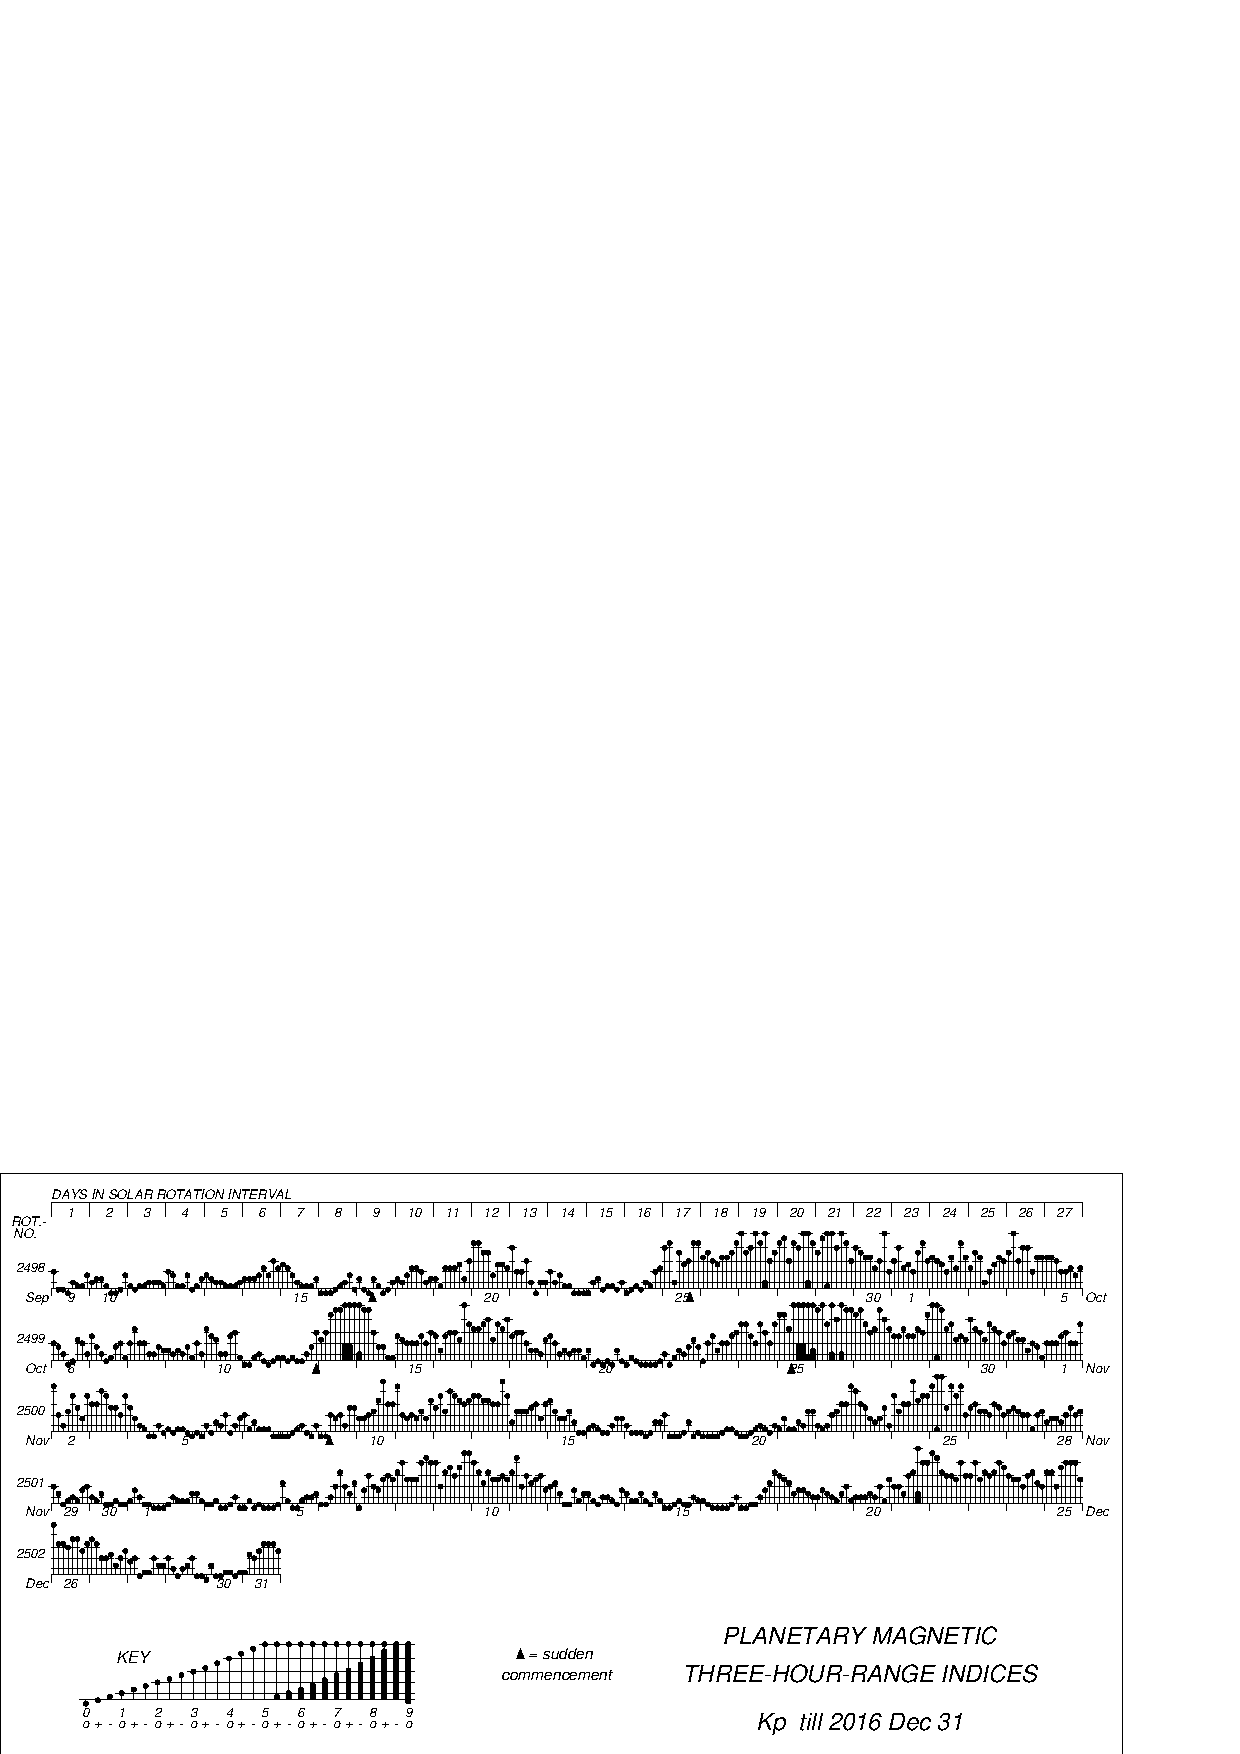
\includegraphics[width=\textwidth]{images/musi1612.pdf}
	\caption{Bartels musical \Kp{} diagram for the time period from September until end of December 2016. Two sudden commencements with following geomagnetic storms, having a maximal \Kp{} of $6+$, can be seen in October. Credit: \href{http://www.gfz-potsdam.de/en/kp-index/}{GFZ~Potsdam}, 2017, licensed under \href{https://creativecommons.org/licenses/by/4.0/}{CC BY 4.0}.}
	\label{fig:musi1612}
\end{figure}
%ftp://ftp.gfz-potsdam.de/pub/home/obs/kp-ap/music/

The \Kp{}~index can be converted to the 3"~hour equivalent $ap$~index, which represents the magnetic field strength at a surface position of about \SI{50}{\degree} dipole latitude. The conversion is done via a table defined by Bartels, in which the value of the \textit{ap}~index is scaled in units of \SI{2}{nT} (see \autoref{tab:kp_to_ap_table}).
\begin{table}
	\caption{Defined table for the conversion from the \Kp~index to the equivalent \textit{ap}~index, which represents the magnetic field strength in units of \SI{2}{nT}.}
	\label{tab:kp_to_ap_table}
	\centering
	\begin{tabular}{lssssssssssssss}
		\Kp	&0o	&0+	&1-	&1o	&1+	&2-	&2o	&2+	&3-	&3o	&3+	&4-	&4o	&4+\\
		\textit{ap}	&0	&2	&3	&4	&5	&6	&7	&9	&12	&15	&18	&22	&27	&32\\
		\hline
		\Kp	&5-	&5o	&5+	&6-	&6o	&6+	&7-	&7o	&7+	&8-	&8o	&8+	&9-	&9o\\
		\textit{ap}	&39	&48	&56	&67	&80	&94	&111	&132	&154	&179	&207	&236	&300	&400
	\end{tabular}
\end{table}
There are further geomagnetic indices which are derived from the \Kp{}~index. They include $Ap$, the daily $ap$ average, $Cp$, the daily $ap$ sum mapped via a defined table to the range \numrange{0}{2.5}, and $C9$, a mapping of $Cp$ via a defined table to the range \numrange{0}{9}. The definitions of Q"~days (quiet days) and D"~days (disturbed days) are also obtained from the \Kp{}~index.

The International Association of Geomagnetism and Aeronomy (IAGA) adopted the \Kp{}~index in 1954. The \Kp{}~index was maintained in Göttingen until January 1997 -- now the German Research Centre for Geosciences (GFZ) in Potsdam supplies the \Kp{}~index and thereof derived indices. The GFZ provides historical and quicklook data of the indices via their website\footnote{GFZ website for geomagnetic indices: \url{http://www.gfz-potsdam.de/de/kp-index/} (existent in 2017-10-29)}. The data was extended backwards and is available from 1932 onwards.\\

Several indicators/quantities are based on the \Kp{}~index:\\
The NOAA G-Scale for geomagnetic storms (G~1 to G~5) is based on the \Kp~index\footnote{NOAA Space Weather Scales website: \url{http://www.swpc.noaa.gov/noaa-scales-explanation} (existent in 2017-10-29)}.\\
The equatorward auroral boundary position correlates with the \Kp~index (cite?).\\
The variation of the total electron content (TEC) of the ionosphere correlates with the \Kp~index (cite?). The TEC has influence on global navigation satellite systems (GNSS). A part of their positional error scales directly with TEC (in extreme cases up to about \SI{30}{\m}).\\

"It is designed to measure solar particle radiation by its magnetic effects."\\

Because of the effects on sensitive technical systems, methods for \Kp{} forecasting are developed.\\
- Wing \Kp{} model (link)\\
- Potsdam quicklook data (link)\\
- Alexej \Kp{} correlation forecast model (link)\\
- In this work we derive relations for \Kp{} nowcast from in-situ solar-wind measurements and \Kp{} forecast from remote solar-wind stream/CME observations.\\

% acknowledgments:\\
% The results presented in this thesis rely on the \Kp{}~index, calculated and made available by the German Research Centre for Geosciences in Potsdam from data collected at magnetic observatories. We thank the involved national institutes, the INTERMAGNET network and ISGI (isgi.unistra.fr).\\


\subsection{OMNI data set}
\label{sec:omni_data_set}

see paper...\\

a data set merged from different sources\\
The OMNI data \citep{King2005} were obtained from the GSFC/SPDF OMNIWeb interface.\\

from spacecraft located near the Lagrange point L1 upstream of Earth\\
time-shifted to the bow shock of the magnetosphere\\

OMNI2 H0 MRG1HR (1963--201308)
Cite from CDAweb: Hourly near-Earth solar-wind magnetic field and plasma data, energetic proton fluxes (>~1 to >~60~MeV), and geomagnetic and solar activity indices.

NASA, Goddard Space Flight Center (GSFC), Space Physics Data Facility (SPDF): \url{http://spdf.gsfc.nasa.gov/}\\	%exintent in 2016-08-18
- Coordinated Data Analysis Web (CDAWeb): \url{http://cdaweb.gsfc.nasa.gov/}\\	%exintent in 2016-08-18
- OMNIWeb Plus: \url{http://omniweb.gsfc.nasa.gov/}\\	%exintent in 2016-08-18
%OMNIWeb Data Documentation: http://omniweb.gsfc.nasa.gov/html/ow_data.html

intercalibrated multi-spacecraft solar-wind data\\
Various spacecraft contribute to the interplanetary magnetic field (IMF) and solar-wind plasma OMNI data, as seen in \autoref{fig:timeline_OMNI_SC_IDs}.\\
\begin{figure}[htb]
	\centering
	\includegraphics[width=\textwidth]{images/gnuplots/timeline_OMNI_SC_IDs.pdf}
	\caption{IMF and solar-wind plasma data source spacecraft for the high and the low resolution OMNI (HRO, LRO) data sets until end of 2016. The SIDC 13-month smoothed monthly SSN is plotted in the background. add cycle number...}
	\label{fig:timeline_OMNI_SC_IDs}
\end{figure}

\subsubsection{Solar Wind Structures}
Solar Wind Structures (SWS) list\\
derived by Richardson.... from OMNI data (only?)
see chapter2...\\

permission received.\\

%http://cedarweb.vsp.ucar.edu/wiki/index.php/Tools_and_Models:Solar_Wind_Structures
characterization of near-Earth solar-wind structures since 1963\\
SWS lists \citep{Richardson2000} and \citep{Richardson2012}


\subsection{Helios probes}
\label{sec:helios_probes}

see Helios data readme.txt\\
see paper\\

two different fluxgate magnetometers and a search coil magnetometer\\

see \autoref{fig:helios2}
\begin{figure}[htb]
	\begin{floatrow}
		\ffigbox[\FBwidth][]{
			\includegraphics[width=0.3\textwidth]{images/helios2.jpg}
		}{
			\caption{One of the nearly identical twin Helios spacecraft. Credit: \href{https://solarsystem.nasa.gov/galleries/helios}{NASA/Max Planck Institute for Solar System Research}.}
			\label{fig:helios2}
			%source: https://solarsystem.nasa.gov/galleries/helios
			%NASA has no copyrights to its contents
		}
		\ffigbox[\Xhsize]{
			\includegraphics{images/gnuplots/Helios12_1h_r_b_ssn_plot.pdf}
		}{
			\caption{Plot of the Helios probes' solar distance and HGI latitude over their mission time, together with the monthly SSN and 13-month smoothed monthly SSN.}
			\label{fig:Helios12_1h_r_b_ssn_plot}
		}
	\end{floatrow}
\end{figure}

solar distance, HGI latitude and sunspot number during the Helios missions; see \autoref{fig:Helios12_1h_r_b_ssn_plot}\\

Helios~1 and 2 orbits in the ecliptic plane and in the latitude polar plane (see \autoref{fig:Helios12_orbits_ecliptic_polar})\\
\begin{figure}[htb]
	\centering
	\includegraphics[width=\textwidth]{images/gnuplots/Helios12_orbits_ecliptic_polar.pdf}
	\caption{Orbits of the Helios~1 (red) and Helios~2 (green) spacecraft in the solar equatorial plane (left) and polar plane (right) (HGI-coordinates). change colors?}
	\label{fig:Helios12_orbits_ecliptic_polar}
\end{figure}

The Helios magnetic field and plasma data frequency over heliocentric distance and over heliographic latitude are plotted in \autoref{fig:helios_data_frequency}.\\
\begin{figure}[htb]
	\centering
	\includegraphics[width=\textwidth]{images/gnuplots/helios_data_frequency.pdf}
	\caption{Helios data frequency over heliocentric distance with bins of \SI{0.01}{au} (left panels) and over heliographic latitude with bins of \SI{0.1}{\degree} (right panels). The frequency data is based on the hourly merged magnetometer and plasma data sets for Helios~1 and Helios~2. The top panels show the frequencies for Helios~1 and Helios~2 individually and the bottom panels those for the magnetometer and plasma data. avoid white lines...}
	\label{fig:helios_data_frequency}
\end{figure}

Solar wind data courtesy of R.~Schwenn, Max-Planck-Institut für Aeronomie, Lindau, magnetic field data courtesy of F.~Neubauer, Universität zu Köln. (see paper; into acknowledgements...)\\

%see presi 1.07 Inside Helios-Origins and Evolution-Salem.ppt
%see book Schwenn1990 https://books.google.de/books?id=W1DuCAAAQBAJ&printsec=frontcover&dq=Physics+of+the+Inner+Heliosphere+I.+Large-Scale+Phenomena&hl=de&sa=X&redir_esc=y#v=onepage&q=Physics%20of%20the%20Inner%20Heliosphere%20I.%20Large-Scale%20Phenomena&f=false



data sources -- see paper for replacing the following data\\
solar-wind parameters: ACE, Helios, OMNI\\
geomagnetic indices: Kp, OMNI\\

Space Physics Data Facility (SPDF)\\

HELIOS~1 and 2 - orbital Parameters\\
\url{http://spdf.sci.gsfc.nasa.gov/pub/data/helios/helios1/traj/}\\
\url{http://spdf.sci.gsfc.nasa.gov/pub/data/helios/helios2/traj/}\\

Helios hourly merged mag \& plasma data:\\
HELIOS1\_COHO1HR\_MERGED\_MAG\_PLASMA\_2965.txt\\
HELIOS2\_COHO1HR\_MERGED\_MAG\_PLASMA\_3096.txt\\
\url{http://cdaweb.gsfc.nasa.gov}\\
temporal coverage of merged data\\
Helios 1: 1974-12-10 - 1981-06-14\\
Mag data availability: 42.6~\%\\
Plasma \& orbit data availability: 76.4~\%\\
Helios 2: 1976-01-01 - 1980-03-04\\
Mag data availability: 54.4~\%\\
Plasma \& orbit data availability: 91.8~\%\\


\subsection{Real-time solar-wind data}

Advanced Composition Explorer (ACE)\\
s/c figure, launch date was 25 August 1997\\

Wind, STEREO, SOHO, CELIAS\\

data errors/gaps...\\
Several services/alerts are based on the data streams from real-time measurements. (L1 alerts, etc.)\\

DSCOVR as replacement was launched on 11~Februar 2015. It is NOAA's SWPC real-time solar-wind prime source since 27 July 2016.\footnote{\url{http://www.swpc.noaa.gov/products/real-time-solar-wind}}\\
		%introduction, basics and data

	%####--  Chapter2  --####
	%\chapter{Chapter2}
%\section{Abstract}

\titley{Solar wind predictions for the Parker Solar Probe orbit}
\subtitley{Near-Sun extrapolations derived from an empirical solar wind model based on Helios and OMNI observations}

% \author{M.~S.~Venzmer
% \and V.~Bothmer}
% 
% \institute{University of Goettingen, Institute for Astrophysics, Friedrich-Hund-Platz~1, 37077~Göttingen, Germany}
% 
% \date{Received 25 August 2017; accepted date}
% %First draft 9 August 2016; first changes 21 June 2017; second changes 17 July 2017; third changes 17 August 2017; fourth changes 24 August 2017; submitted 25 August 2017

\abstracty
{The Parker Solar Probe (PSP) (formerly Solar Probe Plus) mission will be humanity’s first in situ exploration of the solar corona with closest perihelia at \num{9.86}~solar radii (\si{\Rs}) distance to the Sun. It will help answer hitherto unresolved questions on the heating of the solar corona and the source and acceleration of the solar wind and solar energetic particles. The scope of this study is to model the solar wind environment for PSP’s unprecedented distances \textbf{in} its prime mission phase during the years \numrange{2018}{2025}. The study is performed within the project Coronagraphic German And US \textbf{SolarProbePlus} Survey (CGAUSS) which is the German contribution to the PSP mission as part of the Wide-field Imager for Solar PRobe (WISPR).}	%context
{We present an empirical solar wind model for the inner heliosphere which is derived from OMNI and Helios data. The German-US space probes Helios~1 and Helios~2 flew in the 1970s and observed solar wind in the ecliptic within heliocentric distances of \SIrange{0.29}{0.98}{\au}. The OMNI database consists of multi-spacecraft intercalibrated in situ data obtained near \SI{1}{\au} over more than five solar cycles. The international sunspot number (SSN) and its predictions are used to derive dependencies of the major solar wind parameters on solar activity and to forecast their properties for the PSP mission.}	%aims
{The frequency distributions for the solar wind key parameters magnetic field strength, proton velocity, density and temperature are represented by lognormal functions. In addition, we consider the velocity distribution’s bi-componental shape, consisting of a slower and a faster part. Functional relations to solar activity are compiled with use of the OMNI data by correlating and fitting the frequency distributions with the SSN. Further, based on the combined data set from both Helios probes, the parameters’ frequency distributions are fitted with respect to solar distance to obtain power law dependencies. Thus an empirical solar wind model for the inner heliosphere confined to the ecliptic region is derived, accounting for solar activity and for solar distance through adequate shifts of the lognormal distributions. Finally, the inclusion of SSN predictions and the extrapolation \textbf{down} to PSP’s perihelion \textbf{region} enables us to estimate the solar wind environment for PSP’s planned trajectory during its mission duration.}	%methods
{The CGAUSS empirical solar wind model for PSP yields dependencies \textbf{on solar activity and solar distance for the solar wind parameters' frequency distributions}. The estimated solar wind median values for PSP’s first perihelion in 2018 at a solar distance of \SI{0.16}{\au} are \SI{87}{\nT}, \SI{340}{\km\per\s}, \SI{214}{\per\cm\cubed} and \SI{503000}{\K}. The estimates for PSP’s \textbf{first closest perihelion, occuring} in 2024 at \SI{0.046}{\au} (\SI{9.86}{\Rs}), are \SI{943}{\nT}, \SI{290}{\km\per\s}, \SI{2951}{\per\cm\cubed} and \SI{1930000}{\K}. \textbf{Since the modeled velocity and temperature values below about \SI{20}{\Rs} appear overestimated in comparison with existing observations, this suggests that PSP will directly measure solar wind acceleration and heating processes below \SI{20}{\Rs} as planned. } }	%results
{}	%conclusions

% \keywords{solar wind -- sun: heliosphere -- sun: corona}
% 
% \maketitle

%\titlerunning{Solar wind extrapolation to PSP orbit}
%\authorrunning{Venzmer \& Bothmer}


%title and abstract for submitting:

%Solar wind predictions for the Parker Solar Probe orbit
%Near-Sun extrapolations derived from an empirical solar wind model based on Helios and OMNI observations

%The Parker Solar Probe (PSP) (formerly Solar Probe Plus) mission will be humanity’s first in situ exploration of the solar corona with closest perihelia at 9.86 solar radii (Rs) distance to the Sun. It will help answer hitherto unresolved questions on the heating of the solar corona and the source and acceleration of the solar wind and solar energetic particles. The scope of this study is to model the solar wind environment for PSP’s unprecedented distances during its prime mission phase during the years 2018--2025. The study is performed within the project Coronagraphic German And US Solar Probe Survey (CGAUSS) which is the German contribution to the PSP mission as part of the Wide field Imager for Solar PRobe (WISPR).
%We present an empirical solar wind model for the inner heliosphere which is derived from OMNI and Helios data. The German-US space probes Helios 1 and Helios 2 flew in the 1970s and observed solar wind in the ecliptic within heliocentric distances of 0.29--0.98 au. The OMNI database consists of multi-spacecraft intercalibrated in situ data obtained near 1 au over more than five solar cycles. The international sunspot number (SSN) and its predictions are used to derive dependencies of the major solar wind parameters on solar activity and to forecast their properties for the PSP mission.
%The frequency distributions for the solar wind key parameters magnetic field strength, proton velocity, density and temperature are represented by lognormal functions. In addition, we consider the velocity distribution’s bi-componental shape, consisting of a slower and a faster part. Functional relations to solar activity are compiled with use of the OMNI data by correlating and fitting the frequency distributions with the SSN. Further, based on the combined data set from both Helios probes, the parameters’ frequency distributions are fitted with respect to solar distance to obtain power law dependencies. Thus an empirical solar wind model for the inner heliosphere confined to the ecliptic region is derived, accounting for solar activity and for solar distance through adequate shifts of the lognormal distributions. Finally, the inclusion of SSN predictions and the extrapolation to PSP’s perihelion enables us to estimate the solar wind environment for PSP’s planned trajectory during its mission duration.
%The CGAUSS empirical solar wind model for PSP yields dependencies of the solar wind parameters on solar activity and radial distance. The estimated solar wind median values for PSP’s first perihelion in 2018 at a solar distance of 0.16 au are 87 nT, 340 km s-1, 4015 cm-3 and 503000 K. The estimates for PSP’s closest perihelia, beginning in 2024 at 0.046 au (9.86 Rs), are 943 nT, 290 km s-1, 9733 cm-3 and 1930000 K. Though, the modeled velocity and temperature values below about 20 Rs appear overestimated in comparison with existing observations. Thus, PSP is expected to directly measure solar wind acceleration and heating processes below 20 Rs as planned.

%\tableofcontents

\section{Introduction}
%motivation
It is long known (since the early 19th~century) that variations in the solar wind evoke disturbances in the magnetosphere \citep{Bartels1962}. Especially strong disturbances, called geomagnetic storms, can be provoked by coronal mass ejections (CMEs), which are embedded within the solar wind. The causes of the strongest geomagnetic storms are the compression of the solar wind magnetic field lines within the CME shock front and the in CMEs enclosed magnetic clouds with their enhanced field strenghts \citep{Bothmer1993}.

These strong geomagnetic disturbances are a threat to sensitive technical systems and exposed humans. Therefore it is important to know when magnetospheric disturbances will occur and how large they will be.\\

%aim
The goal of this paper is to estimate the magnetospheric impact of solar wind in general and to predict it for CMEs in particular.\\


%outline of structure
First we determine the magnitudes of the long-time \Kp{} changes due to solar activity (Sect.~...) and second we measure the extent of seasonal variations stemming from the Earth's orbit (Sect.~...).\\

%general solar wind nowcast
In situ measurements of solar wind are made almost continuously (e.g., at the first Lagrange point (L1)) in front of the magnetosphere. Since 1963 several spacecraft collected more than 50~years of data. The latest spacecraft, e.g., Wind, ACE and DSCOVR (launched in early 2015), provide real-time solar wind data.\footnote{Wind: \url{https://pwg.gsfc.nasa.gov/windnrt/}} \footnote{ACE: \url{http://www.swpc.noaa.gov/products/ace-real-time-solar-wind}} \footnote{DSCOVR: \url{http://www.swpc.noaa.gov/products/real-time-solar-wind}}

This real-time data can be used to estimate various solar wind effects, e.g., the position of the magnetospheric bow shock in front of the Earth, the magnitude of geomagnetic disturbances (\Kp~index), the positions of the polar auroral ovals, the variation of the total electron content (TEC) of the ionosphere, the positional error of global navigation satellite systems (GNSS),...\\

The equatorward auroral boundary position correlates with the \Kp~index.\\

The total electron content (TEC) of the ionosphere has influence on global navigation satellite systems (GNSS). A part of their positional error scales directly with the TEC (in extreme cases up to about \SI{30}{\m}).\\

%CME velocity forecast
The velocity and direction of CMEs can be determined in their early near-Sun stages via remote tracking with coronagraph white-light observations. Using these parameters as input for propagation models, their possible arrival time and arrival velocity at Earth can be derived.\\

%stream velocity forecast from CHs
As coronal holes are the origin of the fast solar wind, their area on the solar disk, seen in EUV images, correlates with the measured velocity of solar wind streams \citep{Vrsnak2007}. This is used to predict the Earth arrival velocity of solar wind streams about 4~days in advance \citep{Rotter2012}.\footnote{\url{http://swe.uni-graz.at/index.php/services/solar-wind-forecast}}\\

With our results presented here we elaborate the step from the predicted CME and stream velocities to the forecast of the possible impact strength on the Earth's magnetosphere.\\

%differences to existing studies
[\citet{Elliott2013}: The \Kp~index and solar wind speed relationship: Insights for improving space weather forecasts]\\

We make an empirical correlation of the solar wind speed with the geomagnetic \Kp~index to obtain the capability to forecast \Kp{} values solely based on the predicted CME and stream velocities.\\

The used OMNI data set consists of minutely data in the time range 1981-01-01 to 2016-12-31.\\

The derived functional dependencies can be used to nowcast/forecast the \Kp~index.\\


%motivation
why use the \Kp{} index?\\


\section{Long-term variations of the \Kp{}~index}

\subsection{\Kp{} data}
The \Kp{} data is obtained from the GFZ~Potsdam\footnote{\url{http://www.gfz-potsdam.de/de/kp-index/}}, where the index is now maintained. The data used in this analysis covers the time period 1932--2016.\\

The \Kp{} frequency distribution for the time period 1932--2016 shows that the highest frequencies occur around low \Kp{} values of 1+ and to higher \Kp{} values the frequencies seem to decline exponentially (see Fig.~\ref{fig:Kp_histogram}). A \Kp{} value of 9o occurred only 29 times in this time interval.\\
\begin{figure}
	\fcapside[\FBwidth]{
		\includegraphics[width=0.5\textwidth]{chapter2/figures/Kp_histogram.pdf}
	}{
		\caption{\Kp{} frequency distribution for the time period 1932--2016. \Kp{} data from the GFZ~Potsdam.}
		\label{fig:Kp_histogram}
	}
\end{figure}

\subsection{\Kp{} variations with solar activity}
solar activity is tracked with the sunspot number (SSN); SSN data\\
The general \Kp{} distribution, seen before in Fig.~\ref{fig:Kp_histogram}, averages over solar activity. With different states of solar activity the \Kp{} frequency distributions' shape varies. This can be seen from the yearly distributions, sorted and colored by yearly SSN (see Fig.~\ref{fig:Kp_histogram_yearlySSN}). The distribution's peak position scales with SSN, that is, a high yearly SSN results also in more large \Kp{} values.\\
\begin{figure}
	\fcapside[\FBwidth]{
		\includegraphics[width=0.5\textwidth]{chapter2/figures/Kp_histogram_yearlySSN.pdf}
	}{
		\caption{Yearly \Kp{} frequency distributions of the period 1932--2016 sorted and colored by SSN. \Kp{} data from the GFZ~Potsdam and the yearly SSN from the SILSO World Data Center.}
		\label{fig:Kp_histogram_yearlySSN}
	}
\end{figure}

The time series of yearly average \Kp{} values in the time span 1932--2016 shows an imprint of the solar cycles (see the top graphs in Fig.~\ref{fig:yearly_kp-ssn_correlation_c}).
\begin{figure}
	\fcapside[\FBwidth]{
		\includegraphics[width=0.5\textwidth]{chapter2/figures/yearly_kp-ssn_correlation_c.pdf}
	}{
		\caption{Yearly \Kp~index from GFZ~Potsdam and yearly SSN from the SILSO World Data Center (1932--2016) with cycle number (top). The correlation coefficients with the yearly SSN are calculated for time lags back to -15~years (bottom).}
		\label{fig:yearly_kp-ssn_correlation_c}
	}
\end{figure}
The \Kp{} pattern follows the solar cycle minima and maxima as well as the changes in magnitude between solar cycles. The yearly mean \Kp{} shifts about 1~unit for both variations.

As expected, the \Kp{}~index correlation with solar activity shows an 11-year period (see bottom graph in Fig.~\ref{fig:yearly_kp-ssn_correlation_c}). The highest correlation coefficient 0.60 is found with a time lag of $-1$~year, that is, the yearly average \Kp{} follows the SSN of the previous year.
%Kp-ssn cc: 0.5971

cause are CHs, see paper...\\

The yearly mean \Kp~indices with respect to the 1-year lagged SSN show a raise in \Kp{} with increasing SSN, which is seen in Fig.~\ref{fig:Kp_SSN_fit_d}.
\begin{figure}
	\fcapside[\FBwidth]{
		\includegraphics[width=0.5\textwidth]{chapter2/figures/Kp_SSN_fit_d.pdf}
	}{
		\caption{Yearly mean \Kp~index over 1-year lagged SSN (+) with the weighted logarithmic fit (dashed). The error bars denote the SSN standard deviation and the relative weight from the yearly data coverage. The shaded area represents the fit error band derived from the estimated standard deviations of the fit parameters. The function (\ref{eq:log_fit_function}) is used for the weighted fit. The yearly \Kp{} mean values are obtained from GFZ~Potsdam data and the yearly SSN from the SILSO World Data Center.}
		\label{fig:Kp_SSN_fit_d}
	}
\end{figure}

We perform a fit to obtain an analytical relation for this dependency. \Kp{} itself is a quasi-logarithmic index, so it is apparent to use a logarithmic fit function:
\begin{align}
	f(x) = a \cdot \ln(x) + b	\,.	\label{eq:log_fit_function}
\end{align}
The fitted parameter values are $a = 0.281(43)$ and $b = 1.05(19)$ and lead to the relation
\begin{align}
	\Kp(ssn) = 0.28 \cdot \ln(ssn) + 1.1	\,.
\end{align}
% log fit parameters:
% a 0.281126         +/- 0.04267
% b 1.04923          +/- 0.19
In the fit result, plotted in Fig.~\ref{fig:Kp_SSN_fit_d}, the mean \Kp{} is 1.05(19) for a SSN of 1 and 2.53(30) for a SSN of 200. The fit error band has a width of about half a \Kp~unit.\\


\subsection{Seasonal \Kp{} variations}
There also are seasonal variations in the magnetospheric disturbances. Looking at the monthly \Kp{} frequency distributions for different seasons of the year, it is apparent that in the months May--August the \Kp{} peak frequency is higher than in the rest of the year (see Fig.~\ref{fig:Kp_histogram_monthly}). In March/April and September/October the \Kp{} values \num{>3} are more abundant.\\
\begin{figure}
	\fcapside[\FBwidth]{
		\includegraphics[width=0.5\textwidth]{chapter2/figures/Kp_histogram_monthly.pdf}
	}{
		\caption{Monthly \Kp{} frequency distributions colored by months of the year. \Kp{} data of the time period 1932--2016 from the GFZ~Potsdam.}
		\label{fig:Kp_histogram_monthly}
	}
\end{figure}
These seasonal \Kp{} changes arise from seasonal variations of the solar wind parameters at Earth, which stem from Earth's yearly changes in orbital distance and heliographic latitude (as discussed in Sect.~XX of MVVB-Paper). Another seasonal effect comes from the Earth's rotation axis tilt (\SI{+-23.44}{\degree}) (obliquity to the ecliptic), which changes the direction of the Earth's magnetic dipole axis to the Sun over the year (see bottom panel of Fig.~\ref{fig:Kp_seasonal}). The rate of magnetic reconnection between solar wind and magnetosphere depends on both fields' direction to each other (parallel/antiparallel) (see Figure in Basics...).\\

\Kp{} seasonal variation effects from seasonal changing Sun tilt, Earth tilt and Earth distance.\\
causes (see citet{Rangarajan1997} p.~1282 and mention Bartels1963 too):\\
- Earth's rotation axis tilt (\SI{+-23.44}{\degree}) (obliquity to orbit/inclination of equator)\\
- solar rotation axis tilt (\SI{+-7.25}{\degree}) (cite 'NASA Earth fact sheet')\\
- Earth's varying solar distance of \SI{+-1.67}{\percent}\\
read Bothmer1998 Ch 3...\\


We quantify the magnitude of these effects. \Kp{} frequency distributions by month, see Fig.~\ref{fig:Kp_seasonal}.\\
\begin{figure}
	\fcapside[\FBwidth]{
		\includegraphics[width=0.5\textwidth]{chapter2/figures/Kp_seasonal.pdf}
	}{
		\caption{\Kp{} frequency distributions by month for the time period 1932--2016 with median and quartile values (top). Solar tilt angle to Earth, Earth tilt angle to Sun and Earth distance to Sun are approximated with trigonometric fuctions (bottom). switch panels...}
		\label{fig:Kp_seasonal}
	}
\end{figure}
for high \Kp{} values (>~4?) there are yearly frequency maxima at the equinoxes and minima at the solstices. this variation amounts to more than 1?~\Kp~unit...\\

The magnitudes of the SSN variation $\Kp(ssn)$ and the seasonal variation \Kp(month) are of a similar order...?\\

Both variations are an indirect influence through solar wind (see paper).\\


\section{\Kp{} nowcast from in situ solar wind measurements}

\subsection{Solar wind-magnetosphere coupling}
%literature
The coupling between the solar wind and the magnetosphere is governed by reconnection and compression of the magnetic field lines (see Basics...).\\

the dayside reconnection is asymmetric\\

To describe this, some coupling functions with different complexity were proposed (Newell, cites? and list).\\

dayside reconnection:\\
``$E_\text{y}$ is the rate at which southward magnetic flux is convected to the magnetosphere by the solar wind ($-v_\text{x} \cdot B_\text{z}$) in GSM coordinates,'' \citep{Russell2007}\\

the product of the proton velocity $v$ and the magnetic field z-component in geocentric solar magnetospheric (GSM) coordinates $B_\text{z}$:
\begin{align}
	?check vectors  E_\text{y} = -v_\text{x} \times B_\text{z}\,\text{(GSM)}	\label{eq:coupling_vxB}
\end{align}
If not specified otherwise, $B_\text{z}$ is always meant to be in GSM coordinates hereafter.\\

argue for \vBz:\\
- 3hmin(\vBz) performs in rank correlation slightly better than the sophisticated Newell formula. really?\\
- simple to calculate\\
- ...\\

We settle for \vBz{} as the coupling function to analyze.\\

It also is known that the solar wind velocity itself already correlates strongly with the \Kp~index. In fact \citet{Machol2013} even proposed a linear function of the \Kp~index as a best proxy for corrupted real-time velocity measurements made by the Advanced Composition Explorer (ACE) spacecraft.\\

\subsection{Data set, data processing and correlation}
\label{sec:data_set__data_processing_and_correlation}
%determine data basis
The \Kp{} time series started in 1932 when there were no spacecraft to measure in situ solar wind. Thus, the surveyed time range is defined by the available in situ solar wind data. The OMNI data set collects the longest continuous solar wind measurements at \SI{1}{\au},
it covers hourly data since 1963; 5-minute and minutely data since 1981.\\

why this data set? - because of long time coverage, to magnetospheric bow shock calculated solar wind and integrated geomagnetic indices (see Paper...)\\

%argue for averaging method
The \Kp{}~index represents maximal variations within 3-hour time intervals. Any solar wind parameter that will be correlated with it also has to have the same time resolution. Additionally to adapting the time resolution, we have to consider by which means it should be done. Simple 3-hour average values should have a lower correlation coefficient than the solar wind parameter's 3-hourly maximal variation.\\

%argue for high resolution, deliberate between hourly and minutely data
The 3-hour maximal variations are obviously higher when using high resolution data. Thus, to be able to correlate \Kp{} with solar wind data, high resolution data (e.g., 1~min) is needed to determine the maximal solar wind variations within each 3-hour interval.\\

%compare data sets (hourly/minutely->what is good for 3hmax?\\
The longest time coverage has the hourly OMNI data set (since 1963), however we prefer to use the minutely OMNI data with the time range 1981--2016, to benefit from higer correlation coefficients (see Figs?).\\

% Velocity-\Kp{} correlation coefficients for maximum, mean and minimum, see Fig.~\ref{fig:cc_lag_data_b}.\\
% \begin{figure}
% 	\resizebox{\hsize}{!}{\includegraphics{chapter2/figures/cc_lag_data_b.pdf}}
% 	\caption{Velocity-\Kp{} correlation coefficients for different time shifts. Hourly and minutely OMNI data from 1981--2016 with max, mean and min averaging.}
% 		\label{fig:cc_lag_data_b}
%	}
% \end{figure}
% 3-hour max data has a higher correlation coefficient than 3-hour mean data. Max averaging achieves highest cc.\\
% hourly data has slightly lower cc's than minutely data. Why? mean of mean is mean.\\

Pearson correlation coefficients; use Spearman rank instead?\\
correlate positive and negative values separately?\\

\Kp{}-\vBz{} Pearson correlation coefficients for mean and minimum, see Fig.~\ref{fig:cc_lag_data_d_KpvsVBzgsm}.\\
\begin{figure}
	\fcapside[\FBwidth]{
		\includegraphics[width=0.5\textwidth]{chapter2/figures/cc_lag_data_d_KpvsVBzgsm.pdf}
	}{
		\caption{\Kp-\vBz{} correlation coefficients for different time shifts. Minutely OMNI data from 1981--2016 processed with mean (black) and minimum (red) 3-hour averaging.}
		\label{fig:cc_lag_data_d_KpvsVBzgsm}
	}
\end{figure}
%highest correlation coefficients:
%min:	0.00000    -0.717240
%mean:	0.00000    -0.362237
%max:	0.00000     0.293137
The largest correlation is found for the 3-hour minimum data without time shift. It is a negative correlation with a coefficient of $-0.72$.\\

We use \vBz{} 3-hour minimum values, as a result their frequency distribution and its peak is asymmetrically shifted to negative values, as seen in Fig.~\ref{fig:histogram_VBzgsm}.\\
\begin{figure}
	\fcapside[\FBwidth]{
		\includegraphics[width=0.5\textwidth]{chapter2/figures/histogram_VBzgsm.pdf}
	}{
		\caption{Frequency distributions of \vBz{} for 3-hour mean (black) and minimum (red) minutely OMNI data from 1981--2016.}
		\label{fig:histogram_VBzgsm}
	}
\end{figure}
%vBz frequency shifts:
% min shift: -1250
% mean shift: -250
% max shift: -750
even the 3-hour mean shows a slight offset in position (why?)\\


\subsection{Functional dependency}
%distribution
The frequency distribution over the \Kp-\vBz{} space is shaped like a candle flame inclined to negative values by a light breeze, see top panel in Fig.~\ref{fig:Kp_2dhistogram_VBzgsm_sws_d}.
\begin{figure}
	\fcapside[\FBwidth]{
		\includegraphics[width=0.5\textwidth]{chapter2/figures/Kp_2dhistogram_VBzgsm_sws_d.pdf}
	}{
		\caption{\Kp{} versus \vBz{} frequency distribution (top) and its relative distribution (bottom) with the mean \Kp{} values (solid) and their mean absolute deviation (dotted). It is 3-hour minimum data from the minutely OMNI data set (1981--2016). The bin size is \SI{500}{\km\per\s\nano\tesla} and \SI{1/3}{\Kp~unit} respectively.}
		\label{fig:Kp_2dhistogram_VBzgsm_sws_d}
	}
\end{figure}

%dependency
To determine a functional dependency we look at the relative frequencies per \vBz-interval and their mean \Kp{} values, which are plotted in the bottom panel of Fig.~\ref{fig:Kp_2dhistogram_VBzgsm_sws_d}. The mean absolute deviation (MAD) of the mean has a mean size of \SI{0.7}{\Kp~units}. This probability distribution is asymmetrically V-shaped around zero, having a larger and steeper negative arm. This effect is not a result of the data reducing method (3-hour minimum), because for 3-hour mean data the asymmetry also exists (fig...?). Rather the steeper negative arm is a consequence of the half-wave rectifier coupling of the solar wind magnetic field direction to the magnetosphere as described in Sect~(coupling section...).\\
%MAD: 2.211/3 = 0.737 Kp units

%determine fitting functions
Since the \Kp~index has a quasi-logarithmic scaling (see Basics...), a logarithmic function is the obvious choice as a fit function. Furthermore, the depending argument consists of a product of two solar wind parameters which individually scale logarithmically with \Kp{}. These reasons are why we use the logarithm of a parabola for the fitting approach:
\begin{align}
	f(x) &= \ln(x^2)	\,.	\label{eq:log_square_function}
\end{align}
We introduce a horizontal shifting parameter $x2$ because the distribution's center is slightly offset. To be able to replicate the asymmetry in both arms, we split the fit function into a negative and a positive part:
\begin{align}
	f(x) &=
	\begin{cases}
		\,f_-(x) &\text{for } x < 0	\,,\\
		\,f_+(x) &\text{for } x \ge 0	\,.
	\end{cases}	\label{eq:log_square_fit_function}
\end{align}
This way both arms can be scaled individually with the scaling factors for the negative and positive parts $a$ and $c$. The resulting logarithmic fit functions are
\begin{align}
	f_-(x) &= a \cdot \ln((x + x2)^2 + d) + b	\,,\\
	f_+(x) &= c \cdot (f_-(x) - f_-(-x2)) + f_-(-x2)	\,,
\end{align}
with the vertical shifting parameter $b$ and the depth parameter $d$.\\

The resulting fit is plotted in Fig.~\ref{fig:Kp_2dhistogram_VBzgsm_sws_fit_e} with the fit coefficients $a = 1.258(19)$, $b = -17.04(33)$, $c = 0.467(20)$, $d = \num{1.416(68)e6}$ and $x2 = 163(20)$ for units of [\si{\km\per\s \nano\tesla}].\\
%high precision values:
% a = 1.25788(0.019)\\
% b = -17.0394(0.33)\\
% c = 0.467039(0.0197)\\
% d = 1.41639e6(0.067795e6)\\
% x2 = 162.907(20.642)\\
\begin{figure}
	\fcapside[\FBwidth]{
		\includegraphics[width=0.5\textwidth]{chapter2/figures/Kp_2dhistogram_VBzgsm_sws_fit_e.pdf}
	}{
		\caption{Mean \Kp{} values (+) and MAD values (dotted) per \vBz~interval. The error bars represent the relative data count. The logarithmic fit (dashed) is plotted with a mean MAD band (shaded area). The splitted function (\ref{eq:log_square_fit_function}) is used for the weighted fit. OMNI data from the time period 1981--2016 is used.}
		\label{fig:Kp_2dhistogram_VBzgsm_sws_fit_e}
	}
\end{figure}

Thus, the solar wind dependency relation condenses to:
\begin{align}
	\text{\Kp}_-(vB_\text{z}) &= 1.26 \cdot \ln((vB_\text{z} + 160)^2 + \num{1.42e6}) - 17.0	\,,	\label{eq:kpvsvbz_dependency_function_negative}\\
	\text{\Kp}_+(vB_\text{z}) &= 0.47 \cdot (\text{\Kp}_-(vB_\text{z}) - \text{\Kp}_-(-160)) + \text{\Kp}_-(-160)	\,.	\label{eq:kpvsvbz_dependency_function_positive}
\end{align}
This relation can be used together with real-time in situ measurements from spacecraft located at L1 to nowcast the actual \Kp~index.\\


\section{\Kp{} forecast from remote CME observations}
Compared to the steady solar wind, which can be measured reliably only from in situ measurements, CMEs can already be sighted raising from their source region on the solar surface. From remote coronagraph observations some CME properties can be estimated and modeled to Earth, like its propagation direction and its arrival time and velocity (cites...). Thus, early observations enable a heads-up time only depending on the CME's propagation speed to Earth. This travel duration can be more than 4~days for slow events with average solar wind speeds, about 40~hours for fast events with average speeds of \SI{1000}{\km\per\s} and down to 20~hours and even below for the rare extreme cases, e.g., 19~hours for the event observed by \citet{Carrington1859} on 1~September 1859 and about 21~hours for the event on 23~July 2012 \citep{Russell2013,Temmer2015}.\\

To make use of the heads-up time for CMEs, we simplify the coupling relation from before (\ref{eq:coupling_vxB}) by neglecting its magnetic field part, which cannot be determined from remote observations. Only the solar wind velocity is left as a coupling parameter.\\

\subsection{CME velocity estimation}
methods and modeling...?\\
GCS, CAD modeling -> propagation direction and apex height-time profile -> acceleration and velocity kinematics...\\
-> example event CME?\\

\subsection{SWS CME list}
For the following analysis we use the list of solar wind structures (SWS) created and updated by \citet{Richardson2000,Richardson2012}, who characterized the near-Earth solar wind structures since 1963. All periods related to ICMEs in the OMNI solar wind data set were identified and flagged.\\

The SWS list for 1963--2016 was kindly provided by Ian~Richardson (private communication).\\

SWS list for 1963--2015 by \citep{Richardson2000,Richardson2012} is available via registration at CEDARweb\footnote{CEDARweb website for Solar Wind Structures: \url{http://cedarweb.vsp.ucar.edu/wiki/index.php/Tools_and_Models:Solar_Wind_Structures} (existent in 2017-10-29)}.\\
List of near-Earth ICMEs since January 1996 by \citet{Cane2003,Richardson2010}. Available as ACE Level~3 data for the period 1995--mid2016\footnote{ACE Level~3 data website -- list of near-Earth ICMEs: \url{http://www.srl.caltech.edu/ACE/ASC/DATA/level3/icmetable2.htm} (existent in 2017-10-29)}.\\

The CME fraction of the OMNI time series for the period 1981--2016 is \SI{15.8}{\%} (5.53~years) and that for the period 1963--2016 is \SI{17.0}{\%} (9.01~years).\\

% acknowledgments:\\
% The hourly solar wind structure list was kindly provided by Ian~Richardson of the NASA Goddard Space Flight Center and CRESST/University of Maryland via the CEDAR Database at the National Center for Atmospheric Research, which is supported by the National Science Foundation.\\


\subsection{Data processing and correlation}
Again we calculate 3-hour extreme values using the minutely OMNI data to profit from higher correlation coefficients, like done for the data processing of the \vBz{} analysis in Sect.~\ref{sec:data_set__data_processing_and_correlation}. For the velocity these are 3-hour maximum values. The comparison between the 3-hour maximum and the 3-hour mean frequency distributions show that their mean position raises from 405 to \SI{425}{\km\per\s}, see Fig.~\ref{fig:histogram_V_b}.\\
%the SWS1 mean raises from 435 to 455~km/s in 3hmax data...\\
\begin{figure}
	\fcapside[\FBwidth]{
		\includegraphics[width=0.5\textwidth]{chapter2/figures/histogram_V_b.pdf}
	}{
		\caption{Solar wind velocity frequency distributions for 3-hour mean (black), maximum (red) and maximum of the CME part (green). Minutely OMNI data from the period 1981--2016 is used.}
		\label{fig:histogram_V_b}
	}
\end{figure}

Using the CME periods from the SWS list as a filter, the CME part and non-CME part of the data can be examined separately. Their frequency distributions show that in faster solar wind the CME share is rising until eventually in the region above about \SI{900}{\km\per\s} there exist only CMEs, see Fig.~\ref{fig:histogram_V_b}.

The CME part of the data is correlated with the \Kp~index independently from the remaining solar wind, see Fig.~\ref{fig:cc_lag_sws_d}.
\begin{figure}
	\fcapside[\FBwidth]{
		\includegraphics[width=0.5\textwidth]{chapter2/figures/cc_lag_sws_d.pdf}
	}{
		\caption{\Kp{}-velocity correlation coefficients for different time shifts. The correlations for the whole solar wind data (solid), for solar wind without CMEs (dashed) and for CMEs only (dotted) are plotted. The used data is the 3-hour maximum of the minutely high resolution OMNI data.}
		\label{fig:cc_lag_sws_d}
	}
\end{figure}
The correlation for CME related data is smaller than that for the regular solar wind. Its maximal correlation coefficient with a value of 0.51 is without time shift, see Table~\ref{tab:correlation_coefficients_kpvsv}.
\begin{table*}
	\caption{Time lags with the highest correlation coefficients for the \Kp{}-velocity relation. The used data is the 3-hour maximum of the minutely high resolution OMNI data.}
	\label{tab:correlation_coefficients_kpvsv}
	\centering
	\begin{tabular}{lcc}
		\hline\hline
		Data	&Time lag [hours]	&Correlation coefficient\\
		\hline
		All data	&6	&0.622\\
		w/o CMEs	&9	&0.661\\
		CMEs	&0	&0.511\\
		\hline
	\end{tabular}
\end{table*}
% the best lag times are:\\
% sws: +6 h\\
% sws1: 0 h\\
% sws23: +9 h\\
% 
% correlation coefficients\\
% SWS1\\
% 0	0.511093\\
% SWS23\\
% lag	cross	auto x	auto y\\
% -3	0.660694\\
% 0	0.620113\\
% SWS\\
% lag	cross	auto x	auto y\\
% -2	0.621539\\
% 0	0.595784\\
The regular solar wind without CMEs shows a higher correlation with \Kp{} and its maximal coefficient of 0.66 is at a positive time shift of 9~hours, that is, the \Kp~index forecasts the velocity of regular solar wind 9~hours in advance.

The positive time shift can be explained with the occurence of interaction regions followed by high speed streams (HSS). When a slow solar wind stream is followed by a fast one, the compression at their interface leads to enhanced solar wind densities and magnetic field strengths. The peak velocity of a HSS naturally appears after the interaction region. Therefore the \Kp-impact of the enhanced magnetic field is correlated with the higher velocity of the HSS, yielding the observed positive time shift.\\


\subsection{Functional dependency for CMEs}
The general \Kp-velocity dependency is apparent in the tilt of its distribution, see top panel of Fig.~\ref{fig:Kp_2dhistogram_V_sws_c}.
\begin{figure}
	\fcapside[\FBwidth]{
		\includegraphics[width=0.5\textwidth]{chapter2/figures/Kp_2dhistogram_V_sws_c.pdf}
	}{
		\caption{\Kp-velocity distributions for the whole solar wind data, for solar wind without CMEs and for CMEs only. The used data is the 3-hour maximum of the minutely high resolution OMNI data. For the CME separation the SWS list from \citet{Richardson2012} is used. The bin size is \SI{10}{\km\per\s} and \SI{1/3}{\Kp~unit} respectively.}
		\label{fig:Kp_2dhistogram_V_sws_c}
	}
\end{figure}
The comparison with the CME data shows that \Kp{} values \num{>7} and velocities \SI{>900}{\km\per\s} are almost always associated with CME related periods, see middle and bottom panel of Fig.~\ref{fig:Kp_2dhistogram_V_sws_c}.\\

To find a functional dependency for the mean \Kp{} value we look at the relative frequencies per velocity interval, which are plotted in the bottom panel of Fig.~\ref{fig:Kp_2dhistogram_V_sws1_c}.
\begin{figure}
	\fcapside[\FBwidth]{
		\includegraphics[width=0.5\textwidth]{chapter2/figures/Kp_2dhistogram_V_sws1_c.pdf}
	}{
		\caption{CME part of the \Kp-velocity distribution (same as third panel of Fig.~\ref{fig:Kp_2dhistogram_V_sws_c}) and its relative distribution per velocity interval with the mean \Kp{} values (solid) and their mean absolute deviation (dotted). The bin size is \SI{10}{\km\per\s} and \SI{1/3}{\Kp~unit} respectively.}
		\label{fig:Kp_2dhistogram_V_sws1_c}
	}
\end{figure}
The mean \Kp{} value seems to scale almost linear with the solar wind velocity. The mean absolute deviation of the mean has a mean size of about \SI{1.1}{\Kp~units}.\\
%MAD: 3.338/3 = 1.113 Kp units

%determine fitting function
Again, as the \Kp~index has a quasi-logarithmic scaling, a logarithmic function is the obvious choice for the fitting process, for which thus the logarithmic function
\begin{align}
	f(x) = a \cdot \ln(x + x1) + b	\label{eq:log_offset_fit_function}
\end{align}
is used, with the scaling factor $a$, the location parameter $x1$ and the vertical shifting parameter $b$.\\

The resulting fit is plotted in Fig.~\ref{fig:Kp_2dhistogram_V_sws1_fit_e}, with velocity in units of [\si{\km\per\s}] its parameters are $a = \num{10.6(34)}$, $b = \num{-73(28)}$ and $x1 = \num{8.1(43)e2}$.\\
%10.6075 (3.4)\\
%-73.1694 (28.)\\
%806.943 (430)\\
\begin{figure}
	\fcapside[\FBwidth]{
		\includegraphics[width=0.5\textwidth]{chapter2/figures/Kp_2dhistogram_V_sws1_fit_e.pdf}
	}{
		\caption{Mean \Kp{} values (+) and MAD values (dotted) per velocity interval for the CME part of the data. The error bars represent the relative data count. The logarithmic fit (dashed) is plotted with a mean MAD band (shaded area). The function (\ref{eq:log_offset_fit_function}) is used for the weighted fit. The CME part of the OMNI data from the period 1981--2016 is obtained using the SWS list from \citet{Richardson2012}.}
		\label{fig:Kp_2dhistogram_V_sws1_fit_e}
	}
\end{figure}
This leads to the CME dependency function
\begin{align}
	\Kp(v) = 11 \cdot \ln(v + 800) - 70	\,,	\label{eq:kpvsv_dependency_function}
\end{align}
which can be used to forecast the \Kp{}~index from the estimated CME arrival velocity.\\

\subsection{Functional dependency for non-CMEs}

use of by 9-hours shifted data..., see Fig.~\ref{fig:cc_lag_sws_d}\\

To find a functional dependency for the mean \Kp{} value we look at the relative frequencies per velocity interval, which are plotted in the bottom panel of Fig.~\ref{fig:Kp_2dhistogram_V_sws23_c}.
\begin{figure}
	\fcapside[\FBwidth]{
		\includegraphics[width=0.5\textwidth]{chapter2/figures/Kp_2dhistogram_V_sws23_c.pdf}
	}{
		\caption{Non-CME part of the \Kp-velocity distribution (similar to second panel of Fig.~\ref{fig:Kp_2dhistogram_V_sws_c}, but with the by 9-hours shifted data) and its relative distribution per velocity interval with the mean \Kp{} values (solid) and their mean absolute deviation (dotted). The bin size is \SI{10}{\km\per\s} and \SI{1/3}{\Kp~unit} respectively.}
		\label{fig:Kp_2dhistogram_V_sws23_c}
	}
\end{figure}
The mean \Kp{} value seems to scale almost linear with the solar wind velocity. The mean absolute deviation of the mean has a mean size of about \SI{0.7}{\Kp~units}.\\
%MAD: 2.226/3 = 0.742 Kp units
%MAD: 2.332/3 = 0.777 Kp units for 300--900km/s
%MAD: 2.389/3 = 0.796 Kp units for 350--900km/s
%MAD: 2.454/3 = 0.818 Kp units for 350--850km/s

%determine fitting function
Again, as the \Kp~index has a quasi-logarithmic scaling, a logarithmic function is the obvious choice for the fitting process, for which thus the logarithmic function (\ref{eq:log_offset_fit_function}) is used.\\

The resulting fit is plotted in Fig.~\ref{fig:Kp_2dhistogram_V_sws23_fit_e} and the fit parameters are $a = \num{5.88(38)}$, $b = \num{-3.70(29)e1}$ and $x1 = \num{2.99(49)e2}$, with velocity in units of [\si{\km\per\s}].\\
%a1 = 5.88(38)
%b1 = -37.0(29)
%x1 = 299(49)
\begin{figure}
	\fcapside[\FBwidth]{
		\includegraphics[width=0.5\textwidth]{chapter2/figures/Kp_2dhistogram_V_sws23_fit_e.pdf}
	}{
		\caption{Mean \Kp{} values (+) and MAD values (dotted) per velocity interval for the non-CME part of the data, shifted by 9-hours. The error bars represent the relative data count. The logarithmic fit (dashed) is plotted with a mean MAD band (shaded area). The function (\ref{eq:log_offset_fit_function}) is used for the weighted fit. The non-CME part of the OMNI data from the period 1981--2016 is obtained using the SWS list from \citet{Richardson2012}.}
		\label{fig:Kp_2dhistogram_V_sws23_fit_e}
	}
\end{figure}
This leads to the non-CME dependency function
\begin{align}
	\Kp(v) = 5.9 \cdot \ln(v + 300) - 37	\,,	\label{eq:kpvsv_sws23_dependency_function}
\end{align}
which can be used to forecast the \Kp{}~index from the estimated velocity coming from coronal hole analysis.\\


\section{Results and discussion}
solar activity: \Kp-$ssn$ relation\\
seasonal changes: \Kp{}-month relation\\
solar wind nowcast: \Kp-\vBz{} relation (average and worst case)\\
CME forecast: \Kp-velocity relation (average and worst case)\\
non-CME forecast: \Kp-velocity relation (average and worst case)\\

\Kp-velocity correlation\\
similar to \citet{Elliott2013}; different data time period, resolution and averaging method (3-hour maximum of 1~min data)\\


\section{Conclusions}

\section{Outlook}

Applications:\\
\Kp-rssfeed, realtime solar wind and \Kp{} plot\\
CME \Kp{} impact (part of UGOE DDC)\\
give URLs...\\

%\section{Acknowledgments}

\chapter*{Acknowledgements}
\addcontentsline{toc}{chapter}{\texorpdfstring{\color{gray}Acknowledgements}{Acknowledgements}}
%\addchap{\texorpdfstring{\color{gray}Acknowledgments}{Acknowledgments2}}
%\addchap{\hyperref[sec:toc]{\color{gray}Acknowledgments}}

% personal acknowledgements
There are some people I want to thank, without whom the realization and results of my thesis certainly would have been different.
% Volker
First and foremost, I thank my PhD supervisor Volker~Bothmer for supervising my doctorate, for letting me work so freely, and for providing helpful discussions and comments.
% thesis committee
I am grateful to Volker~Bothmer and Ansgar~Reiners for constituting my advisory committee and also for kindly agreeing to evaluate my work as thesis committee.
% further committee members
% I thank the further committee members Andreas~Tilgner, XXX, XXX, and XXX who kindly agreed to evaluate my thesis defense.

% IAG
My appreciation goes to all members of the Institute for Astrophysics for facilitating such a pleasant work environment.
I thank all current and former associates of the space weather group for their friendly company on my way -- in particular Jens, Johannes, Niclas, and Giuseppe for our lively discussions, which were every now and then even scientifically motivated ;)

% my office mates
I especially thank my eternal office mates Eckhard, Jonas, and Adam:
Eckhard for instantly integrating me at the start of my PhD and the good friendship since,
Jonas for the interesting debates during the beginning,
and Adam for accompanying me through the last difficulties on the way.

I acknowledge the office for cozily accomodating me all the long hours, especially the couch for giving me strength, and the Shadow Worker for guarding the office. I honor the brands Star~Wars and LEGO for providing lots of merchandise and distractions.

% family and friends
I am grateful to my family and friends for supporting me at all times.
% else
Those who are not mentioned above but deserve it are thanked hereby as well.
% Sun
A shout-out to the Sun for creating the solar wind and harboring all life we know of (yet).\\

(I am thankful to the proofreaders for reading drafts of this manuscript and providing very helpful comments and suggestions. Volker, Adam, and Tal?)\\


-------------\\
% academic acknowledgments

for creating and making scientific data available:\\
- SWS list (see Acknowledgements in Elliott2013; directly Ian~Richardson)\\
- OMNI data (see paper)\\
- ACE data\\
- Helios data (see paper)\\
- Kp data\\
- SSN data\\

I acknowledge financial support from the following projects:\\
AFFECTS: Solar wind correlation with magnetosphere\\
CGAUSS: Solar wind model and extrapolation\\
HELCATS: Minimum variance analyses of magnetic clouds\\
OPTIMAP: Solar wind ACE time series\\


This work was done within the scope of the CGAUSS project, funded by the German Aerospace Center (grant number...).\\
The authors thank the Helios and OMNI teams for creating and making availabe the solar wind in situ data. The Helios and the OMNI data sets were supplied by the Space Physics Data Facility at NASA's Goddard Space Flight Center.\\
We thank the 'referees' for /important comments and suggestions. /careful review of this paper.\\

facilities/persons which made available the Helios and OMNI data\\
``Ian Richardson and Hilary Cane for making their Interplanetary Coronal Mass Ejection list readily available''\\
``Joseph King and Natalia Papitashvili for creating the combined OMNI data set''\\
The OMNI data were downloaded from NASA's Space Physics Data Facility ...\\
``We thank the reviewers for the careful review of this paper''\\
The Authors extend their thanks to the referee for important comments and suggestions.\\
This work was supported by the DLR CGAUSS project\\
This work has been done in the frame of the CGAUSS project (url), funded by the DLR\\
We would like to thank the Helios team and NASA's SPDF for supplying the plasma and magnetic field data (url)\\


The results presented in this thesis rely on the \Kp{}~index, calculated and made available by the German Research Centre for Geosciences in Potsdam from data collected at magnetic observatories. We thank the involved national institutes, the INTERMAGNET network and ISGI (isgi.unistra.fr).\\



acknowledgements to MAG/SWEPAM Team for ACE data in basics plots...\\

Helios data acknowledgments:\\
Solar wind data courtesy of R.~Schwenn, Max-Planck-Institut für Aeronomie, Lindau, magnetic field data courtesy of F.~Neubauer, Universität zu Köln. (see paper...)\\

Data acknowledgments for \autoref{chap:chapter2}:\\
%\section{Acknowledgments}
The research leading to these results has received funding from the European Union's Seventh Framework Programme (FP7/2007-2013) under the grant agreement number 263506 (AFFECTS). The results presented in this paper rely on the \Kp{}~index, calculated and made available by the German Research Centre for Geosciences in Potsdam from data collected at magnetic observatories. We thank the involved national institutes, the INTERMAGNET network and ISGI (isgi.unistra.fr). The authors thank the OMNI PIs/teams for creating and making available the solar wind in-situ data. The OMNI data are supplied by the NASA Space Science Data Coordinated Archive and the Space Physics Data Facility at NASA's Goddard Space Flight Center. Additional thanks for maintaining and providing the international sunspot number series goes to the World Data Center -- Sunspot Index and Long-term Solar Observations at the Solar Influences Data Analysis Center (SIDC), Royal Observatory of Belgium. The update of the hourly solar wind structure list was kindly provided by Ian~Richardson of the NASA Goddard Space Flight Center and CRESST/University of Maryland via the CEDAR Database at the National Center for Atmospheric Research, which is supported by the National Science Foundation.\\

% NASA ADS
This research has made use of NASA's Astrophysics Data System Bibliographic Services.\\




%search & replace for figures:
%figures/ -> chapter2/figures/


	
\chapter{notes to chapter2...}

% Alle Presis ausschlachten!\\
% Alle Projektberichte ausschlachten!\\
% Kp8--Liste irgendwo einweben...\\

-> example events CIR/HSS and CME\\

%the relation of these events was confirmed two decades ago by (who and \citet{Bothmer1993})\\


\section{Solar wind structure analyses}
How strong do different structure types influence the terrestrial magnetosphere?\\
What kind of solar wind structures create the individual regions in this distribution?\\
What is their individual contribution to the Kp ranges (e.g. high Kp: CMEs 70\% and CIRs 30\%)?\\

ACE solar wind time series and event list\\
sw-timeseries ACE OPTIMAP ``Zeitreihe''-events

method: automatic list creation by event detection via parameter thresholds...\\

sample CME analyses (MVA -> Kp)\\


\section{Forecast}
How can the impact field strength of CMEs be forecasted (V->B correlation for CMEs)?\\
Internal solar wind correlations:\\
B-V correlation\\
ACE MAGSWE 64~s data -> yearly overlay plot\\

applications:\\
rssfeeds, rtsw plots\\
CME Kp impact as part of DDC\\
- \textit{Kp} nowcast with L1 solar wind measurements (L1 alerts, disseminated as RSS feeds; integrated in smartphone app and space weather display)\\
- Forecast of the possible CME impact on the Earth's magnetosphere (\textit{Kp} index) from the predicted CME arrival velocity (integrated in UGOE CME forecast chain (aka DDC))\\



	\chapter{Solar wind time variations}
\section{Solar wind variation with solar cycle}
\section{Solar wind variation with season}
\section{Solar wind empirical forecast}

\chapter{Solar wind distance variations}
\section{Solar wind back-extrapolation}


%COFI -- chapter outline and flow integration\\

see paper...\\

McGregor2011 analyzed the empirical magnetic topology–velocity relationship, using Helios perihelion data with the Wang-Sheeley-Arge (WSA) coronal model, and found indications, that the fast and slow solar wind are generated from distinct sources. (not only superradial expansion)\\


	
	%####--  PaperMVVB  --####
	
% paper issue: first page toc links wrong because of openright option of includepdf
% make openright manually with newpage
\newpage
replace paper with actual published A\&A version...\\
\newpage


\includepdf[pages={-},addtotoc={
1,chapter,1,Paper: Solar-wind predictions for the Parker Solar Probe orbit,chap:solar_wind_predictions_for_the_parker_solar_probe_orbit,
1,subsection,3,Abstract,sec:abstract,
1,section,2,Introduction,sec:introduction,
2,section,2,Frequency distributions of the solar-wind parameters,sec:frequency_distributions_of_the_solar_wind_parameters,
3,section,2,Solar activity dependence of the solar-wind frequency distributions,sec:solar_activity_dependence_of_the_solar_wind_frequency_distributions,
6,section,2,Solar distance dependency,sec:solar_distance_dependency,
9,section,2,Empirical solar-wind model,sec:empirical_solar_wind_model,
10,section,2,Model extrapolation to PSP orbit,sec:model_extrapolation_to_psp_orbit,
12,section,2,Discussion and summary,sec:discussion_and_summary,
13,subsection,3,References,sec:references
}]{paperMVVB/aa31831-17.pdf}


	%%\chapter{PaperMVVB}
%\section{Abstract}

\titley{Solar wind predictions for the Parker Solar Probe orbit}
\subtitley{Near-Sun extrapolations derived from an empirical solar wind model based on Helios and OMNI observations}

% \author{M.~S.~Venzmer
% \and V.~Bothmer}
% 
% \institute{University of Goettingen, Institute for Astrophysics, Friedrich-Hund-Platz~1, 37077~Göttingen, Germany}
% 
% \date{Received 25 August 2017; accepted date}
% %First draft 9 August 2016; first changes 21 June 2017; second changes 17 July 2017; third changes 17 August 2017; fourth changes 24 August 2017; submitted 25 August 2017

\abstracty
{The Parker Solar Probe (PSP) (formerly Solar Probe Plus) mission will be humanity’s first in situ exploration of the solar corona with closest perihelia at \num{9.86}~solar radii (\si{\Rs}) distance to the Sun. It will help answer hitherto unresolved questions on the heating of the solar corona and the source and acceleration of the solar wind and solar energetic particles. The scope of this study is to model the solar wind environment for PSP’s unprecedented distances \textbf{in} its prime mission phase during the years \numrange{2018}{2025}. The study is performed within the project Coronagraphic German And US \textbf{SolarProbePlus} Survey (CGAUSS) which is the German contribution to the PSP mission as part of the Wide-field Imager for Solar PRobe (WISPR).}	%context
{We present an empirical solar wind model for the inner heliosphere which is derived from OMNI and Helios data. The German-US space probes Helios~1 and Helios~2 flew in the 1970s and observed solar wind in the ecliptic within heliocentric distances of \SIrange{0.29}{0.98}{\au}. The OMNI database consists of multi-spacecraft intercalibrated in situ data obtained near \SI{1}{\au} over more than five solar cycles. The international sunspot number (SSN) and its predictions are used to derive dependencies of the major solar wind parameters on solar activity and to forecast their properties for the PSP mission.}	%aims
{The frequency distributions for the solar wind key parameters magnetic field strength, proton velocity, density and temperature are represented by lognormal functions. In addition, we consider the velocity distribution’s bi-componental shape, consisting of a slower and a faster part. Functional relations to solar activity are compiled with use of the OMNI data by correlating and fitting the frequency distributions with the SSN. Further, based on the combined data set from both Helios probes, the parameters’ frequency distributions are fitted with respect to solar distance to obtain power law dependencies. Thus an empirical solar wind model for the inner heliosphere confined to the ecliptic region is derived, accounting for solar activity and for solar distance through adequate shifts of the lognormal distributions. Finally, the inclusion of SSN predictions and the extrapolation \textbf{down} to PSP’s perihelion \textbf{region} enables us to estimate the solar wind environment for PSP’s planned trajectory during its mission duration.}	%methods
{The CGAUSS empirical solar wind model for PSP yields dependencies \textbf{on solar activity and solar distance for the solar wind parameters' frequency distributions}. The estimated solar wind median values for PSP’s first perihelion in 2018 at a solar distance of \SI{0.16}{\au} are \SI{87}{\nT}, \SI{340}{\km\per\s}, \SI{214}{\per\cm\cubed} and \SI{503000}{\K}. The estimates for PSP’s \textbf{first closest perihelion, occuring} in 2024 at \SI{0.046}{\au} (\SI{9.86}{\Rs}), are \SI{943}{\nT}, \SI{290}{\km\per\s}, \SI{2951}{\per\cm\cubed} and \SI{1930000}{\K}. \textbf{Since the modeled velocity and temperature values below about \SI{20}{\Rs} appear overestimated in comparison with existing observations, this suggests that PSP will directly measure solar wind acceleration and heating processes below \SI{20}{\Rs} as planned. } }	%results
{}	%conclusions

% \keywords{solar wind -- sun: heliosphere -- sun: corona}
% 
% \maketitle

%\titlerunning{Solar wind extrapolation to PSP orbit}
%\authorrunning{Venzmer \& Bothmer}


%title and abstract for submitting:

%Solar wind predictions for the Parker Solar Probe orbit
%Near-Sun extrapolations derived from an empirical solar wind model based on Helios and OMNI observations

%The Parker Solar Probe (PSP) (formerly Solar Probe Plus) mission will be humanity’s first in situ exploration of the solar corona with closest perihelia at 9.86 solar radii (Rs) distance to the Sun. It will help answer hitherto unresolved questions on the heating of the solar corona and the source and acceleration of the solar wind and solar energetic particles. The scope of this study is to model the solar wind environment for PSP’s unprecedented distances during its prime mission phase during the years 2018--2025. The study is performed within the project Coronagraphic German And US Solar Probe Survey (CGAUSS) which is the German contribution to the PSP mission as part of the Wide field Imager for Solar PRobe (WISPR).
%We present an empirical solar wind model for the inner heliosphere which is derived from OMNI and Helios data. The German-US space probes Helios 1 and Helios 2 flew in the 1970s and observed solar wind in the ecliptic within heliocentric distances of 0.29--0.98 au. The OMNI database consists of multi-spacecraft intercalibrated in situ data obtained near 1 au over more than five solar cycles. The international sunspot number (SSN) and its predictions are used to derive dependencies of the major solar wind parameters on solar activity and to forecast their properties for the PSP mission.
%The frequency distributions for the solar wind key parameters magnetic field strength, proton velocity, density and temperature are represented by lognormal functions. In addition, we consider the velocity distribution’s bi-componental shape, consisting of a slower and a faster part. Functional relations to solar activity are compiled with use of the OMNI data by correlating and fitting the frequency distributions with the SSN. Further, based on the combined data set from both Helios probes, the parameters’ frequency distributions are fitted with respect to solar distance to obtain power law dependencies. Thus an empirical solar wind model for the inner heliosphere confined to the ecliptic region is derived, accounting for solar activity and for solar distance through adequate shifts of the lognormal distributions. Finally, the inclusion of SSN predictions and the extrapolation to PSP’s perihelion enables us to estimate the solar wind environment for PSP’s planned trajectory during its mission duration.
%The CGAUSS empirical solar wind model for PSP yields dependencies of the solar wind parameters on solar activity and radial distance. The estimated solar wind median values for PSP’s first perihelion in 2018 at a solar distance of 0.16 au are 87 nT, 340 km s-1, 4015 cm-3 and 503000 K. The estimates for PSP’s closest perihelia, beginning in 2024 at 0.046 au (9.86 Rs), are 943 nT, 290 km s-1, 9733 cm-3 and 1930000 K. Though, the modeled velocity and temperature values below about 20 Rs appear overestimated in comparison with existing observations. Thus, PSP is expected to directly measure solar wind acceleration and heating processes below 20 Rs as planned.

%\tableofcontents

\section{Introduction}
%motivation
It is long known (since the early 19th~century) that variations in the solar wind evoke disturbances in the magnetosphere \citep{Bartels1962}. Especially strong disturbances, called geomagnetic storms, can be provoked by coronal mass ejections (CMEs), which are embedded within the solar wind. The causes of the strongest geomagnetic storms are the compression of the solar wind magnetic field lines within the CME shock front and the in CMEs enclosed magnetic clouds with their enhanced field strenghts \citep{Bothmer1993}.

These strong geomagnetic disturbances are a threat to sensitive technical systems and exposed humans. Therefore it is important to know when magnetospheric disturbances will occur and how large they will be.\\

%aim
The goal of this paper is to estimate the magnetospheric impact of solar wind in general and to predict it for CMEs in particular.\\


%outline of structure
First we determine the magnitudes of the long-time \Kp{} changes due to solar activity (Sect.~...) and second we measure the extent of seasonal variations stemming from the Earth's orbit (Sect.~...).\\

%general solar wind nowcast
In situ measurements of solar wind are made almost continuously (e.g., at the first Lagrange point (L1)) in front of the magnetosphere. Since 1963 several spacecraft collected more than 50~years of data. The latest spacecraft, e.g., Wind, ACE and DSCOVR (launched in early 2015), provide real-time solar wind data.\footnote{Wind: \url{https://pwg.gsfc.nasa.gov/windnrt/}} \footnote{ACE: \url{http://www.swpc.noaa.gov/products/ace-real-time-solar-wind}} \footnote{DSCOVR: \url{http://www.swpc.noaa.gov/products/real-time-solar-wind}}

This real-time data can be used to estimate various solar wind effects, e.g., the position of the magnetospheric bow shock in front of the Earth, the magnitude of geomagnetic disturbances (\Kp~index), the positions of the polar auroral ovals, the variation of the total electron content (TEC) of the ionosphere, the positional error of global navigation satellite systems (GNSS),...\\

The equatorward auroral boundary position correlates with the \Kp~index.\\

The total electron content (TEC) of the ionosphere has influence on global navigation satellite systems (GNSS). A part of their positional error scales directly with the TEC (in extreme cases up to about \SI{30}{\m}).\\

%CME velocity forecast
The velocity and direction of CMEs can be determined in their early near-Sun stages via remote tracking with coronagraph white-light observations. Using these parameters as input for propagation models, their possible arrival time and arrival velocity at Earth can be derived.\\

%stream velocity forecast from CHs
As coronal holes are the origin of the fast solar wind, their area on the solar disk, seen in EUV images, correlates with the measured velocity of solar wind streams \citep{Vrsnak2007}. This is used to predict the Earth arrival velocity of solar wind streams about 4~days in advance \citep{Rotter2012}.\footnote{\url{http://swe.uni-graz.at/index.php/services/solar-wind-forecast}}\\

With our results presented here we elaborate the step from the predicted CME and stream velocities to the forecast of the possible impact strength on the Earth's magnetosphere.\\

%differences to existing studies
[\citet{Elliott2013}: The \Kp~index and solar wind speed relationship: Insights for improving space weather forecasts]\\

We make an empirical correlation of the solar wind speed with the geomagnetic \Kp~index to obtain the capability to forecast \Kp{} values solely based on the predicted CME and stream velocities.\\

The used OMNI data set consists of minutely data in the time range 1981-01-01 to 2016-12-31.\\

The derived functional dependencies can be used to nowcast/forecast the \Kp~index.\\


%motivation
why use the \Kp{} index?\\


\section{Long-term variations of the \Kp{}~index}

\subsection{\Kp{} data}
The \Kp{} data is obtained from the GFZ~Potsdam\footnote{\url{http://www.gfz-potsdam.de/de/kp-index/}}, where the index is now maintained. The data used in this analysis covers the time period 1932--2016.\\

The \Kp{} frequency distribution for the time period 1932--2016 shows that the highest frequencies occur around low \Kp{} values of 1+ and to higher \Kp{} values the frequencies seem to decline exponentially (see Fig.~\ref{fig:Kp_histogram}). A \Kp{} value of 9o occurred only 29 times in this time interval.\\
\begin{figure}
	\fcapside[\FBwidth]{
		\includegraphics[width=0.5\textwidth]{chapter2/figures/Kp_histogram.pdf}
	}{
		\caption{\Kp{} frequency distribution for the time period 1932--2016. \Kp{} data from the GFZ~Potsdam.}
		\label{fig:Kp_histogram}
	}
\end{figure}

\subsection{\Kp{} variations with solar activity}
solar activity is tracked with the sunspot number (SSN); SSN data\\
The general \Kp{} distribution, seen before in Fig.~\ref{fig:Kp_histogram}, averages over solar activity. With different states of solar activity the \Kp{} frequency distributions' shape varies. This can be seen from the yearly distributions, sorted and colored by yearly SSN (see Fig.~\ref{fig:Kp_histogram_yearlySSN}). The distribution's peak position scales with SSN, that is, a high yearly SSN results also in more large \Kp{} values.\\
\begin{figure}
	\fcapside[\FBwidth]{
		\includegraphics[width=0.5\textwidth]{chapter2/figures/Kp_histogram_yearlySSN.pdf}
	}{
		\caption{Yearly \Kp{} frequency distributions of the period 1932--2016 sorted and colored by SSN. \Kp{} data from the GFZ~Potsdam and the yearly SSN from the SILSO World Data Center.}
		\label{fig:Kp_histogram_yearlySSN}
	}
\end{figure}

The time series of yearly average \Kp{} values in the time span 1932--2016 shows an imprint of the solar cycles (see the top graphs in Fig.~\ref{fig:yearly_kp-ssn_correlation_c}).
\begin{figure}
	\fcapside[\FBwidth]{
		\includegraphics[width=0.5\textwidth]{chapter2/figures/yearly_kp-ssn_correlation_c.pdf}
	}{
		\caption{Yearly \Kp~index from GFZ~Potsdam and yearly SSN from the SILSO World Data Center (1932--2016) with cycle number (top). The correlation coefficients with the yearly SSN are calculated for time lags back to -15~years (bottom).}
		\label{fig:yearly_kp-ssn_correlation_c}
	}
\end{figure}
The \Kp{} pattern follows the solar cycle minima and maxima as well as the changes in magnitude between solar cycles. The yearly mean \Kp{} shifts about 1~unit for both variations.

As expected, the \Kp{}~index correlation with solar activity shows an 11-year period (see bottom graph in Fig.~\ref{fig:yearly_kp-ssn_correlation_c}). The highest correlation coefficient 0.60 is found with a time lag of $-1$~year, that is, the yearly average \Kp{} follows the SSN of the previous year.
%Kp-ssn cc: 0.5971

cause are CHs, see paper...\\

The yearly mean \Kp~indices with respect to the 1-year lagged SSN show a raise in \Kp{} with increasing SSN, which is seen in Fig.~\ref{fig:Kp_SSN_fit_d}.
\begin{figure}
	\fcapside[\FBwidth]{
		\includegraphics[width=0.5\textwidth]{chapter2/figures/Kp_SSN_fit_d.pdf}
	}{
		\caption{Yearly mean \Kp~index over 1-year lagged SSN (+) with the weighted logarithmic fit (dashed). The error bars denote the SSN standard deviation and the relative weight from the yearly data coverage. The shaded area represents the fit error band derived from the estimated standard deviations of the fit parameters. The function (\ref{eq:log_fit_function}) is used for the weighted fit. The yearly \Kp{} mean values are obtained from GFZ~Potsdam data and the yearly SSN from the SILSO World Data Center.}
		\label{fig:Kp_SSN_fit_d}
	}
\end{figure}

We perform a fit to obtain an analytical relation for this dependency. \Kp{} itself is a quasi-logarithmic index, so it is apparent to use a logarithmic fit function:
\begin{align}
	f(x) = a \cdot \ln(x) + b	\,.	\label{eq:log_fit_function}
\end{align}
The fitted parameter values are $a = 0.281(43)$ and $b = 1.05(19)$ and lead to the relation
\begin{align}
	\Kp(ssn) = 0.28 \cdot \ln(ssn) + 1.1	\,.
\end{align}
% log fit parameters:
% a 0.281126         +/- 0.04267
% b 1.04923          +/- 0.19
In the fit result, plotted in Fig.~\ref{fig:Kp_SSN_fit_d}, the mean \Kp{} is 1.05(19) for a SSN of 1 and 2.53(30) for a SSN of 200. The fit error band has a width of about half a \Kp~unit.\\


\subsection{Seasonal \Kp{} variations}
There also are seasonal variations in the magnetospheric disturbances. Looking at the monthly \Kp{} frequency distributions for different seasons of the year, it is apparent that in the months May--August the \Kp{} peak frequency is higher than in the rest of the year (see Fig.~\ref{fig:Kp_histogram_monthly}). In March/April and September/October the \Kp{} values \num{>3} are more abundant.\\
\begin{figure}
	\fcapside[\FBwidth]{
		\includegraphics[width=0.5\textwidth]{chapter2/figures/Kp_histogram_monthly.pdf}
	}{
		\caption{Monthly \Kp{} frequency distributions colored by months of the year. \Kp{} data of the time period 1932--2016 from the GFZ~Potsdam.}
		\label{fig:Kp_histogram_monthly}
	}
\end{figure}
These seasonal \Kp{} changes arise from seasonal variations of the solar wind parameters at Earth, which stem from Earth's yearly changes in orbital distance and heliographic latitude (as discussed in Sect.~XX of MVVB-Paper). Another seasonal effect comes from the Earth's rotation axis tilt (\SI{+-23.44}{\degree}) (obliquity to the ecliptic), which changes the direction of the Earth's magnetic dipole axis to the Sun over the year (see bottom panel of Fig.~\ref{fig:Kp_seasonal}). The rate of magnetic reconnection between solar wind and magnetosphere depends on both fields' direction to each other (parallel/antiparallel) (see Figure in Basics...).\\

\Kp{} seasonal variation effects from seasonal changing Sun tilt, Earth tilt and Earth distance.\\
causes (see citet{Rangarajan1997} p.~1282 and mention Bartels1963 too):\\
- Earth's rotation axis tilt (\SI{+-23.44}{\degree}) (obliquity to orbit/inclination of equator)\\
- solar rotation axis tilt (\SI{+-7.25}{\degree}) (cite 'NASA Earth fact sheet')\\
- Earth's varying solar distance of \SI{+-1.67}{\percent}\\
read Bothmer1998 Ch 3...\\


We quantify the magnitude of these effects. \Kp{} frequency distributions by month, see Fig.~\ref{fig:Kp_seasonal}.\\
\begin{figure}
	\fcapside[\FBwidth]{
		\includegraphics[width=0.5\textwidth]{chapter2/figures/Kp_seasonal.pdf}
	}{
		\caption{\Kp{} frequency distributions by month for the time period 1932--2016 with median and quartile values (top). Solar tilt angle to Earth, Earth tilt angle to Sun and Earth distance to Sun are approximated with trigonometric fuctions (bottom). switch panels...}
		\label{fig:Kp_seasonal}
	}
\end{figure}
for high \Kp{} values (>~4?) there are yearly frequency maxima at the equinoxes and minima at the solstices. this variation amounts to more than 1?~\Kp~unit...\\

The magnitudes of the SSN variation $\Kp(ssn)$ and the seasonal variation \Kp(month) are of a similar order...?\\

Both variations are an indirect influence through solar wind (see paper).\\


\section{\Kp{} nowcast from in situ solar wind measurements}

\subsection{Solar wind-magnetosphere coupling}
%literature
The coupling between the solar wind and the magnetosphere is governed by reconnection and compression of the magnetic field lines (see Basics...).\\

the dayside reconnection is asymmetric\\

To describe this, some coupling functions with different complexity were proposed (Newell, cites? and list).\\

dayside reconnection:\\
``$E_\text{y}$ is the rate at which southward magnetic flux is convected to the magnetosphere by the solar wind ($-v_\text{x} \cdot B_\text{z}$) in GSM coordinates,'' \citep{Russell2007}\\

the product of the proton velocity $v$ and the magnetic field z-component in geocentric solar magnetospheric (GSM) coordinates $B_\text{z}$:
\begin{align}
	?check vectors  E_\text{y} = -v_\text{x} \times B_\text{z}\,\text{(GSM)}	\label{eq:coupling_vxB}
\end{align}
If not specified otherwise, $B_\text{z}$ is always meant to be in GSM coordinates hereafter.\\

argue for \vBz:\\
- 3hmin(\vBz) performs in rank correlation slightly better than the sophisticated Newell formula. really?\\
- simple to calculate\\
- ...\\

We settle for \vBz{} as the coupling function to analyze.\\

It also is known that the solar wind velocity itself already correlates strongly with the \Kp~index. In fact \citet{Machol2013} even proposed a linear function of the \Kp~index as a best proxy for corrupted real-time velocity measurements made by the Advanced Composition Explorer (ACE) spacecraft.\\

\subsection{Data set, data processing and correlation}
\label{sec:data_set__data_processing_and_correlation}
%determine data basis
The \Kp{} time series started in 1932 when there were no spacecraft to measure in situ solar wind. Thus, the surveyed time range is defined by the available in situ solar wind data. The OMNI data set collects the longest continuous solar wind measurements at \SI{1}{\au},
it covers hourly data since 1963; 5-minute and minutely data since 1981.\\

why this data set? - because of long time coverage, to magnetospheric bow shock calculated solar wind and integrated geomagnetic indices (see Paper...)\\

%argue for averaging method
The \Kp{}~index represents maximal variations within 3-hour time intervals. Any solar wind parameter that will be correlated with it also has to have the same time resolution. Additionally to adapting the time resolution, we have to consider by which means it should be done. Simple 3-hour average values should have a lower correlation coefficient than the solar wind parameter's 3-hourly maximal variation.\\

%argue for high resolution, deliberate between hourly and minutely data
The 3-hour maximal variations are obviously higher when using high resolution data. Thus, to be able to correlate \Kp{} with solar wind data, high resolution data (e.g., 1~min) is needed to determine the maximal solar wind variations within each 3-hour interval.\\

%compare data sets (hourly/minutely->what is good for 3hmax?\\
The longest time coverage has the hourly OMNI data set (since 1963), however we prefer to use the minutely OMNI data with the time range 1981--2016, to benefit from higer correlation coefficients (see Figs?).\\

% Velocity-\Kp{} correlation coefficients for maximum, mean and minimum, see Fig.~\ref{fig:cc_lag_data_b}.\\
% \begin{figure}
% 	\resizebox{\hsize}{!}{\includegraphics{chapter2/figures/cc_lag_data_b.pdf}}
% 	\caption{Velocity-\Kp{} correlation coefficients for different time shifts. Hourly and minutely OMNI data from 1981--2016 with max, mean and min averaging.}
% 		\label{fig:cc_lag_data_b}
%	}
% \end{figure}
% 3-hour max data has a higher correlation coefficient than 3-hour mean data. Max averaging achieves highest cc.\\
% hourly data has slightly lower cc's than minutely data. Why? mean of mean is mean.\\

Pearson correlation coefficients; use Spearman rank instead?\\
correlate positive and negative values separately?\\

\Kp{}-\vBz{} Pearson correlation coefficients for mean and minimum, see Fig.~\ref{fig:cc_lag_data_d_KpvsVBzgsm}.\\
\begin{figure}
	\fcapside[\FBwidth]{
		\includegraphics[width=0.5\textwidth]{chapter2/figures/cc_lag_data_d_KpvsVBzgsm.pdf}
	}{
		\caption{\Kp-\vBz{} correlation coefficients for different time shifts. Minutely OMNI data from 1981--2016 processed with mean (black) and minimum (red) 3-hour averaging.}
		\label{fig:cc_lag_data_d_KpvsVBzgsm}
	}
\end{figure}
%highest correlation coefficients:
%min:	0.00000    -0.717240
%mean:	0.00000    -0.362237
%max:	0.00000     0.293137
The largest correlation is found for the 3-hour minimum data without time shift. It is a negative correlation with a coefficient of $-0.72$.\\

We use \vBz{} 3-hour minimum values, as a result their frequency distribution and its peak is asymmetrically shifted to negative values, as seen in Fig.~\ref{fig:histogram_VBzgsm}.\\
\begin{figure}
	\fcapside[\FBwidth]{
		\includegraphics[width=0.5\textwidth]{chapter2/figures/histogram_VBzgsm.pdf}
	}{
		\caption{Frequency distributions of \vBz{} for 3-hour mean (black) and minimum (red) minutely OMNI data from 1981--2016.}
		\label{fig:histogram_VBzgsm}
	}
\end{figure}
%vBz frequency shifts:
% min shift: -1250
% mean shift: -250
% max shift: -750
even the 3-hour mean shows a slight offset in position (why?)\\


\subsection{Functional dependency}
%distribution
The frequency distribution over the \Kp-\vBz{} space is shaped like a candle flame inclined to negative values by a light breeze, see top panel in Fig.~\ref{fig:Kp_2dhistogram_VBzgsm_sws_d}.
\begin{figure}
	\fcapside[\FBwidth]{
		\includegraphics[width=0.5\textwidth]{chapter2/figures/Kp_2dhistogram_VBzgsm_sws_d.pdf}
	}{
		\caption{\Kp{} versus \vBz{} frequency distribution (top) and its relative distribution (bottom) with the mean \Kp{} values (solid) and their mean absolute deviation (dotted). It is 3-hour minimum data from the minutely OMNI data set (1981--2016). The bin size is \SI{500}{\km\per\s\nano\tesla} and \SI{1/3}{\Kp~unit} respectively.}
		\label{fig:Kp_2dhistogram_VBzgsm_sws_d}
	}
\end{figure}

%dependency
To determine a functional dependency we look at the relative frequencies per \vBz-interval and their mean \Kp{} values, which are plotted in the bottom panel of Fig.~\ref{fig:Kp_2dhistogram_VBzgsm_sws_d}. The mean absolute deviation (MAD) of the mean has a mean size of \SI{0.7}{\Kp~units}. This probability distribution is asymmetrically V-shaped around zero, having a larger and steeper negative arm. This effect is not a result of the data reducing method (3-hour minimum), because for 3-hour mean data the asymmetry also exists (fig...?). Rather the steeper negative arm is a consequence of the half-wave rectifier coupling of the solar wind magnetic field direction to the magnetosphere as described in Sect~(coupling section...).\\
%MAD: 2.211/3 = 0.737 Kp units

%determine fitting functions
Since the \Kp~index has a quasi-logarithmic scaling (see Basics...), a logarithmic function is the obvious choice as a fit function. Furthermore, the depending argument consists of a product of two solar wind parameters which individually scale logarithmically with \Kp{}. These reasons are why we use the logarithm of a parabola for the fitting approach:
\begin{align}
	f(x) &= \ln(x^2)	\,.	\label{eq:log_square_function}
\end{align}
We introduce a horizontal shifting parameter $x2$ because the distribution's center is slightly offset. To be able to replicate the asymmetry in both arms, we split the fit function into a negative and a positive part:
\begin{align}
	f(x) &=
	\begin{cases}
		\,f_-(x) &\text{for } x < 0	\,,\\
		\,f_+(x) &\text{for } x \ge 0	\,.
	\end{cases}	\label{eq:log_square_fit_function}
\end{align}
This way both arms can be scaled individually with the scaling factors for the negative and positive parts $a$ and $c$. The resulting logarithmic fit functions are
\begin{align}
	f_-(x) &= a \cdot \ln((x + x2)^2 + d) + b	\,,\\
	f_+(x) &= c \cdot (f_-(x) - f_-(-x2)) + f_-(-x2)	\,,
\end{align}
with the vertical shifting parameter $b$ and the depth parameter $d$.\\

The resulting fit is plotted in Fig.~\ref{fig:Kp_2dhistogram_VBzgsm_sws_fit_e} with the fit coefficients $a = 1.258(19)$, $b = -17.04(33)$, $c = 0.467(20)$, $d = \num{1.416(68)e6}$ and $x2 = 163(20)$ for units of [\si{\km\per\s \nano\tesla}].\\
%high precision values:
% a = 1.25788(0.019)\\
% b = -17.0394(0.33)\\
% c = 0.467039(0.0197)\\
% d = 1.41639e6(0.067795e6)\\
% x2 = 162.907(20.642)\\
\begin{figure}
	\fcapside[\FBwidth]{
		\includegraphics[width=0.5\textwidth]{chapter2/figures/Kp_2dhistogram_VBzgsm_sws_fit_e.pdf}
	}{
		\caption{Mean \Kp{} values (+) and MAD values (dotted) per \vBz~interval. The error bars represent the relative data count. The logarithmic fit (dashed) is plotted with a mean MAD band (shaded area). The splitted function (\ref{eq:log_square_fit_function}) is used for the weighted fit. OMNI data from the time period 1981--2016 is used.}
		\label{fig:Kp_2dhistogram_VBzgsm_sws_fit_e}
	}
\end{figure}

Thus, the solar wind dependency relation condenses to:
\begin{align}
	\text{\Kp}_-(vB_\text{z}) &= 1.26 \cdot \ln((vB_\text{z} + 160)^2 + \num{1.42e6}) - 17.0	\,,	\label{eq:kpvsvbz_dependency_function_negative}\\
	\text{\Kp}_+(vB_\text{z}) &= 0.47 \cdot (\text{\Kp}_-(vB_\text{z}) - \text{\Kp}_-(-160)) + \text{\Kp}_-(-160)	\,.	\label{eq:kpvsvbz_dependency_function_positive}
\end{align}
This relation can be used together with real-time in situ measurements from spacecraft located at L1 to nowcast the actual \Kp~index.\\


\section{\Kp{} forecast from remote CME observations}
Compared to the steady solar wind, which can be measured reliably only from in situ measurements, CMEs can already be sighted raising from their source region on the solar surface. From remote coronagraph observations some CME properties can be estimated and modeled to Earth, like its propagation direction and its arrival time and velocity (cites...). Thus, early observations enable a heads-up time only depending on the CME's propagation speed to Earth. This travel duration can be more than 4~days for slow events with average solar wind speeds, about 40~hours for fast events with average speeds of \SI{1000}{\km\per\s} and down to 20~hours and even below for the rare extreme cases, e.g., 19~hours for the event observed by \citet{Carrington1859} on 1~September 1859 and about 21~hours for the event on 23~July 2012 \citep{Russell2013,Temmer2015}.\\

To make use of the heads-up time for CMEs, we simplify the coupling relation from before (\ref{eq:coupling_vxB}) by neglecting its magnetic field part, which cannot be determined from remote observations. Only the solar wind velocity is left as a coupling parameter.\\

\subsection{CME velocity estimation}
methods and modeling...?\\
GCS, CAD modeling -> propagation direction and apex height-time profile -> acceleration and velocity kinematics...\\
-> example event CME?\\

\subsection{SWS CME list}
For the following analysis we use the list of solar wind structures (SWS) created and updated by \citet{Richardson2000,Richardson2012}, who characterized the near-Earth solar wind structures since 1963. All periods related to ICMEs in the OMNI solar wind data set were identified and flagged.\\

The SWS list for 1963--2016 was kindly provided by Ian~Richardson (private communication).\\

SWS list for 1963--2015 by \citep{Richardson2000,Richardson2012} is available via registration at CEDARweb\footnote{CEDARweb website for Solar Wind Structures: \url{http://cedarweb.vsp.ucar.edu/wiki/index.php/Tools_and_Models:Solar_Wind_Structures} (existent in 2017-10-29)}.\\
List of near-Earth ICMEs since January 1996 by \citet{Cane2003,Richardson2010}. Available as ACE Level~3 data for the period 1995--mid2016\footnote{ACE Level~3 data website -- list of near-Earth ICMEs: \url{http://www.srl.caltech.edu/ACE/ASC/DATA/level3/icmetable2.htm} (existent in 2017-10-29)}.\\

The CME fraction of the OMNI time series for the period 1981--2016 is \SI{15.8}{\%} (5.53~years) and that for the period 1963--2016 is \SI{17.0}{\%} (9.01~years).\\

% acknowledgments:\\
% The hourly solar wind structure list was kindly provided by Ian~Richardson of the NASA Goddard Space Flight Center and CRESST/University of Maryland via the CEDAR Database at the National Center for Atmospheric Research, which is supported by the National Science Foundation.\\


\subsection{Data processing and correlation}
Again we calculate 3-hour extreme values using the minutely OMNI data to profit from higher correlation coefficients, like done for the data processing of the \vBz{} analysis in Sect.~\ref{sec:data_set__data_processing_and_correlation}. For the velocity these are 3-hour maximum values. The comparison between the 3-hour maximum and the 3-hour mean frequency distributions show that their mean position raises from 405 to \SI{425}{\km\per\s}, see Fig.~\ref{fig:histogram_V_b}.\\
%the SWS1 mean raises from 435 to 455~km/s in 3hmax data...\\
\begin{figure}
	\fcapside[\FBwidth]{
		\includegraphics[width=0.5\textwidth]{chapter2/figures/histogram_V_b.pdf}
	}{
		\caption{Solar wind velocity frequency distributions for 3-hour mean (black), maximum (red) and maximum of the CME part (green). Minutely OMNI data from the period 1981--2016 is used.}
		\label{fig:histogram_V_b}
	}
\end{figure}

Using the CME periods from the SWS list as a filter, the CME part and non-CME part of the data can be examined separately. Their frequency distributions show that in faster solar wind the CME share is rising until eventually in the region above about \SI{900}{\km\per\s} there exist only CMEs, see Fig.~\ref{fig:histogram_V_b}.

The CME part of the data is correlated with the \Kp~index independently from the remaining solar wind, see Fig.~\ref{fig:cc_lag_sws_d}.
\begin{figure}
	\fcapside[\FBwidth]{
		\includegraphics[width=0.5\textwidth]{chapter2/figures/cc_lag_sws_d.pdf}
	}{
		\caption{\Kp{}-velocity correlation coefficients for different time shifts. The correlations for the whole solar wind data (solid), for solar wind without CMEs (dashed) and for CMEs only (dotted) are plotted. The used data is the 3-hour maximum of the minutely high resolution OMNI data.}
		\label{fig:cc_lag_sws_d}
	}
\end{figure}
The correlation for CME related data is smaller than that for the regular solar wind. Its maximal correlation coefficient with a value of 0.51 is without time shift, see Table~\ref{tab:correlation_coefficients_kpvsv}.
\begin{table*}
	\caption{Time lags with the highest correlation coefficients for the \Kp{}-velocity relation. The used data is the 3-hour maximum of the minutely high resolution OMNI data.}
	\label{tab:correlation_coefficients_kpvsv}
	\centering
	\begin{tabular}{lcc}
		\hline\hline
		Data	&Time lag [hours]	&Correlation coefficient\\
		\hline
		All data	&6	&0.622\\
		w/o CMEs	&9	&0.661\\
		CMEs	&0	&0.511\\
		\hline
	\end{tabular}
\end{table*}
% the best lag times are:\\
% sws: +6 h\\
% sws1: 0 h\\
% sws23: +9 h\\
% 
% correlation coefficients\\
% SWS1\\
% 0	0.511093\\
% SWS23\\
% lag	cross	auto x	auto y\\
% -3	0.660694\\
% 0	0.620113\\
% SWS\\
% lag	cross	auto x	auto y\\
% -2	0.621539\\
% 0	0.595784\\
The regular solar wind without CMEs shows a higher correlation with \Kp{} and its maximal coefficient of 0.66 is at a positive time shift of 9~hours, that is, the \Kp~index forecasts the velocity of regular solar wind 9~hours in advance.

The positive time shift can be explained with the occurence of interaction regions followed by high speed streams (HSS). When a slow solar wind stream is followed by a fast one, the compression at their interface leads to enhanced solar wind densities and magnetic field strengths. The peak velocity of a HSS naturally appears after the interaction region. Therefore the \Kp-impact of the enhanced magnetic field is correlated with the higher velocity of the HSS, yielding the observed positive time shift.\\


\subsection{Functional dependency for CMEs}
The general \Kp-velocity dependency is apparent in the tilt of its distribution, see top panel of Fig.~\ref{fig:Kp_2dhistogram_V_sws_c}.
\begin{figure}
	\fcapside[\FBwidth]{
		\includegraphics[width=0.5\textwidth]{chapter2/figures/Kp_2dhistogram_V_sws_c.pdf}
	}{
		\caption{\Kp-velocity distributions for the whole solar wind data, for solar wind without CMEs and for CMEs only. The used data is the 3-hour maximum of the minutely high resolution OMNI data. For the CME separation the SWS list from \citet{Richardson2012} is used. The bin size is \SI{10}{\km\per\s} and \SI{1/3}{\Kp~unit} respectively.}
		\label{fig:Kp_2dhistogram_V_sws_c}
	}
\end{figure}
The comparison with the CME data shows that \Kp{} values \num{>7} and velocities \SI{>900}{\km\per\s} are almost always associated with CME related periods, see middle and bottom panel of Fig.~\ref{fig:Kp_2dhistogram_V_sws_c}.\\

To find a functional dependency for the mean \Kp{} value we look at the relative frequencies per velocity interval, which are plotted in the bottom panel of Fig.~\ref{fig:Kp_2dhistogram_V_sws1_c}.
\begin{figure}
	\fcapside[\FBwidth]{
		\includegraphics[width=0.5\textwidth]{chapter2/figures/Kp_2dhistogram_V_sws1_c.pdf}
	}{
		\caption{CME part of the \Kp-velocity distribution (same as third panel of Fig.~\ref{fig:Kp_2dhistogram_V_sws_c}) and its relative distribution per velocity interval with the mean \Kp{} values (solid) and their mean absolute deviation (dotted). The bin size is \SI{10}{\km\per\s} and \SI{1/3}{\Kp~unit} respectively.}
		\label{fig:Kp_2dhistogram_V_sws1_c}
	}
\end{figure}
The mean \Kp{} value seems to scale almost linear with the solar wind velocity. The mean absolute deviation of the mean has a mean size of about \SI{1.1}{\Kp~units}.\\
%MAD: 3.338/3 = 1.113 Kp units

%determine fitting function
Again, as the \Kp~index has a quasi-logarithmic scaling, a logarithmic function is the obvious choice for the fitting process, for which thus the logarithmic function
\begin{align}
	f(x) = a \cdot \ln(x + x1) + b	\label{eq:log_offset_fit_function}
\end{align}
is used, with the scaling factor $a$, the location parameter $x1$ and the vertical shifting parameter $b$.\\

The resulting fit is plotted in Fig.~\ref{fig:Kp_2dhistogram_V_sws1_fit_e}, with velocity in units of [\si{\km\per\s}] its parameters are $a = \num{10.6(34)}$, $b = \num{-73(28)}$ and $x1 = \num{8.1(43)e2}$.\\
%10.6075 (3.4)\\
%-73.1694 (28.)\\
%806.943 (430)\\
\begin{figure}
	\fcapside[\FBwidth]{
		\includegraphics[width=0.5\textwidth]{chapter2/figures/Kp_2dhistogram_V_sws1_fit_e.pdf}
	}{
		\caption{Mean \Kp{} values (+) and MAD values (dotted) per velocity interval for the CME part of the data. The error bars represent the relative data count. The logarithmic fit (dashed) is plotted with a mean MAD band (shaded area). The function (\ref{eq:log_offset_fit_function}) is used for the weighted fit. The CME part of the OMNI data from the period 1981--2016 is obtained using the SWS list from \citet{Richardson2012}.}
		\label{fig:Kp_2dhistogram_V_sws1_fit_e}
	}
\end{figure}
This leads to the CME dependency function
\begin{align}
	\Kp(v) = 11 \cdot \ln(v + 800) - 70	\,,	\label{eq:kpvsv_dependency_function}
\end{align}
which can be used to forecast the \Kp{}~index from the estimated CME arrival velocity.\\

\subsection{Functional dependency for non-CMEs}

use of by 9-hours shifted data..., see Fig.~\ref{fig:cc_lag_sws_d}\\

To find a functional dependency for the mean \Kp{} value we look at the relative frequencies per velocity interval, which are plotted in the bottom panel of Fig.~\ref{fig:Kp_2dhistogram_V_sws23_c}.
\begin{figure}
	\fcapside[\FBwidth]{
		\includegraphics[width=0.5\textwidth]{chapter2/figures/Kp_2dhistogram_V_sws23_c.pdf}
	}{
		\caption{Non-CME part of the \Kp-velocity distribution (similar to second panel of Fig.~\ref{fig:Kp_2dhistogram_V_sws_c}, but with the by 9-hours shifted data) and its relative distribution per velocity interval with the mean \Kp{} values (solid) and their mean absolute deviation (dotted). The bin size is \SI{10}{\km\per\s} and \SI{1/3}{\Kp~unit} respectively.}
		\label{fig:Kp_2dhistogram_V_sws23_c}
	}
\end{figure}
The mean \Kp{} value seems to scale almost linear with the solar wind velocity. The mean absolute deviation of the mean has a mean size of about \SI{0.7}{\Kp~units}.\\
%MAD: 2.226/3 = 0.742 Kp units
%MAD: 2.332/3 = 0.777 Kp units for 300--900km/s
%MAD: 2.389/3 = 0.796 Kp units for 350--900km/s
%MAD: 2.454/3 = 0.818 Kp units for 350--850km/s

%determine fitting function
Again, as the \Kp~index has a quasi-logarithmic scaling, a logarithmic function is the obvious choice for the fitting process, for which thus the logarithmic function (\ref{eq:log_offset_fit_function}) is used.\\

The resulting fit is plotted in Fig.~\ref{fig:Kp_2dhistogram_V_sws23_fit_e} and the fit parameters are $a = \num{5.88(38)}$, $b = \num{-3.70(29)e1}$ and $x1 = \num{2.99(49)e2}$, with velocity in units of [\si{\km\per\s}].\\
%a1 = 5.88(38)
%b1 = -37.0(29)
%x1 = 299(49)
\begin{figure}
	\fcapside[\FBwidth]{
		\includegraphics[width=0.5\textwidth]{chapter2/figures/Kp_2dhistogram_V_sws23_fit_e.pdf}
	}{
		\caption{Mean \Kp{} values (+) and MAD values (dotted) per velocity interval for the non-CME part of the data, shifted by 9-hours. The error bars represent the relative data count. The logarithmic fit (dashed) is plotted with a mean MAD band (shaded area). The function (\ref{eq:log_offset_fit_function}) is used for the weighted fit. The non-CME part of the OMNI data from the period 1981--2016 is obtained using the SWS list from \citet{Richardson2012}.}
		\label{fig:Kp_2dhistogram_V_sws23_fit_e}
	}
\end{figure}
This leads to the non-CME dependency function
\begin{align}
	\Kp(v) = 5.9 \cdot \ln(v + 300) - 37	\,,	\label{eq:kpvsv_sws23_dependency_function}
\end{align}
which can be used to forecast the \Kp{}~index from the estimated velocity coming from coronal hole analysis.\\


\section{Results and discussion}
solar activity: \Kp-$ssn$ relation\\
seasonal changes: \Kp{}-month relation\\
solar wind nowcast: \Kp-\vBz{} relation (average and worst case)\\
CME forecast: \Kp-velocity relation (average and worst case)\\
non-CME forecast: \Kp-velocity relation (average and worst case)\\

\Kp-velocity correlation\\
similar to \citet{Elliott2013}; different data time period, resolution and averaging method (3-hour maximum of 1~min data)\\


\section{Conclusions}

\section{Outlook}

Applications:\\
\Kp-rssfeed, realtime solar wind and \Kp{} plot\\
CME \Kp{} impact (part of UGOE DDC)\\
give URLs...\\

%\section{Acknowledgments}

\chapter*{Acknowledgements}
\addcontentsline{toc}{chapter}{\texorpdfstring{\color{gray}Acknowledgements}{Acknowledgements}}
%\addchap{\texorpdfstring{\color{gray}Acknowledgments}{Acknowledgments2}}
%\addchap{\hyperref[sec:toc]{\color{gray}Acknowledgments}}

% personal acknowledgements
There are some people I want to thank, without whom the realization and results of my thesis certainly would have been different.
% Volker
First and foremost, I thank my PhD supervisor Volker~Bothmer for supervising my doctorate, for letting me work so freely, and for providing helpful discussions and comments.
% thesis committee
I am grateful to Volker~Bothmer and Ansgar~Reiners for constituting my advisory committee and also for kindly agreeing to evaluate my work as thesis committee.
% further committee members
% I thank the further committee members Andreas~Tilgner, XXX, XXX, and XXX who kindly agreed to evaluate my thesis defense.

% IAG
My appreciation goes to all members of the Institute for Astrophysics for facilitating such a pleasant work environment.
I thank all current and former associates of the space weather group for their friendly company on my way -- in particular Jens, Johannes, Niclas, and Giuseppe for our lively discussions, which were every now and then even scientifically motivated ;)

% my office mates
I especially thank my eternal office mates Eckhard, Jonas, and Adam:
Eckhard for instantly integrating me at the start of my PhD and the good friendship since,
Jonas for the interesting debates during the beginning,
and Adam for accompanying me through the last difficulties on the way.

I acknowledge the office for cozily accomodating me all the long hours, especially the couch for giving me strength, and the Shadow Worker for guarding the office. I honor the brands Star~Wars and LEGO for providing lots of merchandise and distractions.

% family and friends
I am grateful to my family and friends for supporting me at all times.
% else
Those who are not mentioned above but deserve it are thanked hereby as well.
% Sun
A shout-out to the Sun for creating the solar wind and harboring all life we know of (yet).\\

(I am thankful to the proofreaders for reading drafts of this manuscript and providing very helpful comments and suggestions. Volker, Adam, and Tal?)\\


-------------\\
% academic acknowledgments

for creating and making scientific data available:\\
- SWS list (see Acknowledgements in Elliott2013; directly Ian~Richardson)\\
- OMNI data (see paper)\\
- ACE data\\
- Helios data (see paper)\\
- Kp data\\
- SSN data\\

I acknowledge financial support from the following projects:\\
AFFECTS: Solar wind correlation with magnetosphere\\
CGAUSS: Solar wind model and extrapolation\\
HELCATS: Minimum variance analyses of magnetic clouds\\
OPTIMAP: Solar wind ACE time series\\


This work was done within the scope of the CGAUSS project, funded by the German Aerospace Center (grant number...).\\
The authors thank the Helios and OMNI teams for creating and making availabe the solar wind in situ data. The Helios and the OMNI data sets were supplied by the Space Physics Data Facility at NASA's Goddard Space Flight Center.\\
We thank the 'referees' for /important comments and suggestions. /careful review of this paper.\\

facilities/persons which made available the Helios and OMNI data\\
``Ian Richardson and Hilary Cane for making their Interplanetary Coronal Mass Ejection list readily available''\\
``Joseph King and Natalia Papitashvili for creating the combined OMNI data set''\\
The OMNI data were downloaded from NASA's Space Physics Data Facility ...\\
``We thank the reviewers for the careful review of this paper''\\
The Authors extend their thanks to the referee for important comments and suggestions.\\
This work was supported by the DLR CGAUSS project\\
This work has been done in the frame of the CGAUSS project (url), funded by the DLR\\
We would like to thank the Helios team and NASA's SPDF for supplying the plasma and magnetic field data (url)\\


The results presented in this thesis rely on the \Kp{}~index, calculated and made available by the German Research Centre for Geosciences in Potsdam from data collected at magnetic observatories. We thank the involved national institutes, the INTERMAGNET network and ISGI (isgi.unistra.fr).\\



acknowledgements to MAG/SWEPAM Team for ACE data in basics plots...\\

Helios data acknowledgments:\\
Solar wind data courtesy of R.~Schwenn, Max-Planck-Institut für Aeronomie, Lindau, magnetic field data courtesy of F.~Neubauer, Universität zu Köln. (see paper...)\\

Data acknowledgments for \autoref{chap:chapter2}:\\
%\section{Acknowledgments}
The research leading to these results has received funding from the European Union's Seventh Framework Programme (FP7/2007-2013) under the grant agreement number 263506 (AFFECTS). The results presented in this paper rely on the \Kp{}~index, calculated and made available by the German Research Centre for Geosciences in Potsdam from data collected at magnetic observatories. We thank the involved national institutes, the INTERMAGNET network and ISGI (isgi.unistra.fr). The authors thank the OMNI PIs/teams for creating and making available the solar wind in-situ data. The OMNI data are supplied by the NASA Space Science Data Coordinated Archive and the Space Physics Data Facility at NASA's Goddard Space Flight Center. Additional thanks for maintaining and providing the international sunspot number series goes to the World Data Center -- Sunspot Index and Long-term Solar Observations at the Solar Influences Data Analysis Center (SIDC), Royal Observatory of Belgium. The update of the hourly solar wind structure list was kindly provided by Ian~Richardson of the NASA Goddard Space Flight Center and CRESST/University of Maryland via the CEDAR Database at the National Center for Atmospheric Research, which is supported by the National Science Foundation.\\

% NASA ADS
This research has made use of NASA's Astrophysics Data System Bibliographic Services.\\




%search & replace:
%McComas2008 to McComas200807

%search & replace for figures:
%figures/ -> paperMVVB/figures/


% change table 2:
% 		\multicolumn{2}{l}{\multirow{2}{*}{Parameter}}	&\multicolumn{2}{c}{Median}	&\multicolumn{1}{c}{Mean}	&\multicolumn{1}{c}{SSN lag}\\
% 		\cline{3-4}
% 		\multicolumn{2}{l}{}	&\multicolumn{1}{c}{SSN factor $a_\text{med}$}	&\multicolumn{1}{c}{Baseline $b_\text{med}$}	&\multicolumn{1}{c}{Scaling factor $a_\text{avg}$}	&\multicolumn{1}{c}{[years]}\\
% 		\hline
% 		\multicolumn{2}{l}{Magnetic field [\si{nT}]}	&1.309(19)e-2	&4.285(17)	&8.786(78)e-2	&0\\
% 		\multicolumn{2}{l}{Density [\si{\per\cm\cubed}]}	&3.81(25)e-3	&4.495(26)	&3.050(27)e-1	&6\\
% 		\multicolumn{2}{l}{Temperature [\SI{e4}{\K}]}	&1.974(26)e-2	&5.729(19)	&6.541(28)e-1	&3\\
% 		\hline
% 		\multicolumn{1}{l}{\multirow{2}{*}{Velocity}}	&\multicolumn{1}{c}{$W'_1$}	&\multicolumn{1}{c}{--}	&3.633(12)	&1.008(37)e-2	&\multirow{2}{*}{--}\\
% 		\multicolumn{1}{l}{\multirow{2}{*}{[\SI{e2}{\km\per\s}]}}	&\multicolumn{1}{c}{$W'_2$}	&\multicolumn{1}{c}{--}	&4.831(81)	&2.31(20)e-2	&\\
% 		\cline{2-6}
% 			&\multicolumn{1}{c}{Balance\tablefootmark{a}}	&-1.799(95)e-3	&0.638(32)	&\multicolumn{1}{c}{--}	&3\\
% 		\hline
% 	\end{tabular}
% 	\tablefoot{
% 		\tablefoottext{a}{SSN factor $c_a$ and baseline parameter $c_b$.}
% 	}


%replace in table 3:
%&\multicolumn{1}{c}{Crossing dist.\!}	&\multicolumn{1}{c}{\!\!Yearly var.\!\!}\\

	%\bibliography{paperMVVB/sections/literature_bibtex}
	%\includepdf[pages=-]{paperMVVB/paperMVVB_without_bold.pdf}

	%\chapter{Helios radial line-up passings}

%COFI -- chapter outline and flow integration\\

have a look into Schwenn1984...\\

%motivation
To derive the radial dependence of the solar wind parameters directly, we look at the passings when both Helios spacecraft were radially lined up. In these cases they flew through the same solar wind at different solar distances.\\
(This eliminates the bias of averaging over slow and fast wind streams, like the described model does.)\\
see also \citet{Schwenn1990} p.~156 + p.~122...\\
%Helios line-up mapping techniques -> Schwenn1981 "Two states..." (not findable online after extensive search)

we compare these independently derived radial fit functions to those obtained from the averaging over all solar wind types...\\

%Helios passings, their time and position
There were eight passings when both Helios spacecraft were radially lined-up (see \autoref{fig:Helios12_lineup_positions_v3_pdfcairo_plot}).
\begin{figure}[htb]
	\centering
	\includegraphics[width=0.6\textwidth]{images/gnuplots/Helios12_lineup_positions_v3_pdfcairo_plot.pdf}
	\caption{Schema of the eight spacecraft line-up positions of both Helios probes on their respective orbits. make B\&W... combine with fig 5.15? calibrate text size}
	\label{fig:Helios12_lineup_positions_v3_pdfcairo_plot}
\end{figure}
These points in time, when both probes had no separation in heliographic longitude, are derived from Helios~1 and Helios~2 daily trajectory data (for the data source see Section~XX). The data is linear interpolated to get an hourly resolution. The resulting points in time together with solar distances are listed in \autoref{tab:lineup_in_longitude}.
\begin{table}[htb]\small
	\centering
	\captionsetup{belowskip=4pt}
	\caption{Times when both Helios probes had no separation in heliographic longitude. Their solar distances (inner spacecraft $r_1$, outer spacecraft $r_2$) were in the range 0.291--0.731~au and the maximal inter-probe radial distance d$r$ was 0.229~au. errors in au...}
	\begin{tabular}{ccccccc}
		\toprule
		\multirow{2}{*}{Passing}	&\multirow{2}{*}{Date}	&\multirow{2}{*}{Time}	&\multirow{2}{*}{Inner s/c}	&$r_1$	&$r_2$	&d$r$\\
			&	&	&	&[au]	&[au]	&[au]\\
		\midrule
		1	&1976-03-09	&00:00	&Helios 1	&0.513	&0.731	&0.219\\
		2	&1976-05-02	&14:00	&Helios 2	&0.442	&0.671	&0.229\\
		3	&1976-09-19	&10:00	&Helios 1	&0.457	&0.637	&0.180\\
		4	&1976-10-31	&11:00	&Helios 2	&0.390	&0.576	&0.186\\
		5	&1977-04-02	&12:00	&Helios 1	&0.394	&0.519	&0.125\\
		6	&1977-04-30	&23:00	&Helios 2	&0.337	&0.465	&0.128\\
		7	&1977-10-18	&06:00	&Helios 1	&0.316	&0.345	&0.029\\
		8	&1977-10-25	&19:00	&Helios 2	&0.291	&0.327	&0.035\\
		\bottomrule
	\end{tabular}
	\label{tab:lineup_in_longitude}
\end{table}
%table data from
%file:///home/raid0/mvenzmer/Desktop/astro70/analyses/Helios12_1h_magswe/Helios12_1h_inline/lineup_periods_v3.txt

%excluding period 7 and 8
The last two passings were merely one week apart and the Helios probes flew almost without radial separation because Helios~2 overtook Helios~1 during its perihelion. As we want to analyze the same solar wind at different solar distances, we exclude the passings 7 and 8 from further analyses.\\


%defining line-up requirements
The passing longitude is not the same as the longitude where the solar wind is detected by both spacecraft consecutively. A passing occurs shortly before the points in time when both spacecraft observe the same solar wind. For the outer probe this point in time is shifted by the solar wind's travel time. The travel time depends on the solar wind's velocity and its distance traveled.\\


%calculation of the offset times
Based on the obtained spacecraft line-up time $t_0$ one can calculate the offset times $t_1$ and $t_2$ when the inner and outer spacecraft pass by the same solar wind (see \autoref{fig:Helios12_lineup_calculation_pdfcairo_plot}). At the solar wind line-up longitude the condition
\begin{align}
	t_2 = t_1 + t_\text{sw} \label{eq:lineup_condition}
\end{align}
holds. As the offset times depend on the solar wind travel time between the probes, we need knowledge of the solar wind velocity $v$ for their calculation: $t_\text{sw} = \text{d}r/v$, with the mean radial separation distance d$r$ between the probes.
\begin{figure}[htb]
	\centering
	\includegraphics[width=0.5\textwidth]{images/gnuplots/Helios12_lineup_calculation_pdfcairo_plot.pdf}
	\caption{Illustration of the solar wind line-up longitude situation with the spacecraft line-up time $t_0$, the offset times $t_1$, $t_2$ (at which the spacecraft measure the same solar wind) and the solar wind travel time $t_\text{sw}$. combine with fig 5.14?}
	\label{fig:Helios12_lineup_calculation_pdfcairo_plot}
\end{figure}
%/home/raid0/mvenzmer/Desktop/astro70/analyses/Helios12_1h_magswe/Helios12_1h_inline/Helios12_lineup_calculation_pdfcairo_gps.txt

%calculating t_1
For the calculation of $t_1$ we recall the third Kepler law
\begin{align}
	\frac{{T_1}^2}{{T_2}^2} = \frac{{a_1}^3}{{a_2}^3}
\end{align}
with the orbital periods $T_1$, $T_2$ and the semi-major axes $a_1$, $a_2$. The assumption of circular orbits (why? what error size?) leads to
\begin{align}
	\frac{{t_1}^2}{(t_1 + t_\text{sw})^2} &= \frac{{r_1}^3}{{r_2}^3}	\nonumber\\
	\Leftrightarrow\qquad\qquad	t_1 &= t_\text{sw} \left( \left( \frac{r_1}{r_2} \right)^\frac{3}{2} - 1 \right)^{-1} \label{eq:offset_time}
\end{align}
and finally the offset time $t_1$ only depends on the variable solar wind travel time $t_\text{sw}$.\\

%calculating the offset time from the solar wind velocity
Due to uncertainties in the travel time $t_\text{sw}$ (the solar wind speed $v$ is obviously not a constant) the exact calculation of $t_1$ is imprecise. To get a reliable result we perform two iterations calculating the offset time from the average velocity $\bar{v}$ of the surrounding 2-day period. We use the velocity $\bar{v}_0$ around $t_0$ to calculate the offset time $t'_1$ as a first estimate. As the velocity $\bar{v}'_1$ at $t'_1$ is certainly different, we use this velocity to refine the value and obtain $t_1$. Hence deriving the velocity $\bar{v}_1$ enables us to calculate the solar wind travel time $t_\text{sw}$.

%We have to round the offset times and time shift values to full hours, because we use the hourly merged mag and plasma Helios data set (see Section~XX) for the velocity calculation.
The average velocities are obtained from the hourly merged (mag?) and (plasma?) Helios data set (see Section~XX). The resulting offset times and velocities of both iterations together with the travel times are listed in \autoref{tab:offset_times}.
\begin{table}[htb]\small
	\centering
	\captionsetup{belowskip=4pt}
	\caption{The two iterations of the derived offset times and average velocities. The resulting solar wind travel times have durations of 11--28~hours. errors...}
	\begin{tabular}{cccccccc}
		\toprule
		\multirow{2}{*}{Passing}	&\multirow{2}{*}{Inner s/c}	&$v_0$	&$t'_1$	&$v'_1$	&$t_1$	&$v_1$	&$t_\text{sw}$\\
			&	&[km/s]	&[h]	&[km/s]	&[h]	&[km/s]	&[h]\\
		\midrule
		1	&Helios 1	&659.3	&19.6	&656.9	&19.7	&656.9	&13.9\\
		2	&Helios 2	&436.4	&25.1	&370.9	&29.5	&356.7	&26.7\\
		3	&Helios 1	&482.6	&24.0	&444.0	&26.1	&413.8	&18.1\\
		4	&Helios 2	&302.3	&32.2	&279.9	&34.8	&278.3	&27.8\\
		5	&Helios 1	&507.3	&20.0	&474.8	&21.4	&473.5	&11.0\\
		6	&Helios 2	&321.2	&26.6	&392.6	&21.7	&367.8	&14.5\\
		\bottomrule
	\end{tabular}
	\label{tab:offset_times}
\end{table}
%table data from
%file:///home/raid0/mvenzmer/Desktop/astro70/analyses/Helios12_1h_magswe/Helios12_1h_inline/lineup_periods_v3.txt

%introducing the lag time for arbitrary longitude positions
For the solar wind line-up longitude condition~\eqref{eq:lineup_condition} holds. For all other positions the solar wind measured by the inner spacecraft will not arrive the outer orbit position at the same time as the outer spacecraft does (see \autoref{fig:Helios12_lineup_calculation_delay_pdfcairo_plot}).
\begin{figure}[htb]
	\centering
	\includegraphics[width=0.5\textwidth]{images/gnuplots/Helios12_lineup_calculation_delay_pdfcairo_plot.pdf}
	\caption{Illustration like \autoref{fig:Helios12_lineup_calculation_pdfcairo_plot} but for arbitrary longitude situations a lag time $t_\text{lag}$ comes into play. merge with fig 5.14?}
	\label{fig:Helios12_lineup_calculation_delay_pdfcairo_plot}
\end{figure}
%/home/raid0/mvenzmer/Desktop/astro70/analyses/Helios12_1h_magswe/Helios12_1h_inline/Helios12_lineup_calculation_delay_pdfcairo_gps.txt

Either the spacecraft (negative lag time) or the solar wind (positive lag time) already have passed this position:
\begin{align}
	t_2 = t_1 + t_\text{sw} + t_\text{lag}. \label{eq:lag_time}
\end{align}
This lag time $t_\text{lag}$ is the time difference at which the solar wind is probed by both spacecraft. At the spacecraft line-up longitude ($t_1 = t_2 = 0$) the lag time equals the solar wind travel time and at the solar wind line-up longitude the lag time is zero.\\

%calculation of the +-24 hour solar wind time span
We choose to look at time periods (instead of points in time) around the offset times to derive average solar wind parameters. This helps reducing the influence of solar wind fluctuations.\\

We define the period duration boundaries as when the lag time $t_\text{lag}$ is in the range $\pm24$~h. For the outer spacecraft these periods are almost twice as long as for the inner spacecraft. The calculated period start and end hours (relative to $t_0$) for both spacecraft are listed in \autoref{tab:period_times_coverage} together with the data coverage of these periods.
\begin{table}[htb]\small
	\centering
	\captionsetup{belowskip=4pt}
	\caption{Derived period start and end hours for both spacecraft in relation to the longitude line-up time $t_0$. The corresponding combined data coverage within that period of the magnetic field, velocity, density and temperature is listed as well. instead duration! errors...}
	\begin{tabular}{cccrrccrrc}
		\toprule
		\multirow{3}{*}{Period}	&	&\multicolumn{4}{c}{Inner spacecraft}	&	&\multicolumn{3}{c}{Outer spacecraft}\\
		\cmidrule{3-6}	\cmidrule{8-10}
			&	&\multirow{2}{*}{s/c}	&Start	&End	&Coverage	&	&Start	&End	&Coverage\\
			&	&	&[h]	&[h]	&[\%]	&	&[h]	&[h]	&[\%]\\
		\midrule
		1	&	&Helios 1	&-14.4	&53.8	&73	&	&-24.6	&91.6	&99\\
		2	&	&Helios 2	&3.1	&58.3	&89	&	&5.8	&109.0	&88\\
		3	&	&Helios 1	&-9.2	&65.1	&16	&	&-15.1	&107.2	&10\\
		4	&	&Helios 2	&4.8	&65.2	&59	&	&8.5	&117.0	&87\\
		5	&	&Helios 1	&-25.5	&68.3	&89	&	&-38.5	&103.3	&88\\
		6	&	&Helios 2	&-15.3	&61.7	&93	&	&-24.8	&100.1	&92\\
		\bottomrule
	\end{tabular}
	\label{tab:period_times_coverage}
\end{table}
% %table data from
% %file:///home/raid0/mvenzmer/Desktop/astro70/analyses/Helios12_1h_magswe/Helios12_1h_inline/lineup_periods_v3.txt

%excluding period 3
For period~3 the combined data coverage of the four solar wind parameters is only 16~\% (Helios~1) and 10~\% (Helios~2) respectively. We consider this as insufficient for the continuing analysis and therefore also omit period~3.\\

The five remaining periods are marked in \autoref{fig:Helios12_lineup_period_positions_v3_pdfcairo_plot}.
\begin{figure}[htb]
	\centering
	\includegraphics[width=0.6\textwidth]{images/gnuplots/Helios12_lineup_period_positions_v3_pdfcairo_plot.pdf}
	\caption{Scheme of the line-up periods of both Helios spacecraft on their respective orbits. The corresponding orbit sections which we consider in our analysis are marked in color. These sections span the positions where both spacecraft observed the same solar wind with a maximal lag time of $\pm24$~hours. bw figure?? dotted lines?}
	\label{fig:Helios12_lineup_period_positions_v3_pdfcairo_plot}
\end{figure}

%average values
The average values of the four parameters magnetic field $B$, velocity $v$, density $n$ and temperature $T$ are listed in \autoref{tab:period_means}.
\begin{table}[htb]\small
	\centering
	\captionsetup{belowskip=4pt}
	\caption{Average values of the four solar wind parameters magnetic field, velocity, density and temperature for the individual periods and spacecraft. errors...}
	\begin{tabular}{cccrrrrcrrrr}
		\toprule
		\multirow{3}{*}{Period}	&	&\multicolumn{5}{c}{Inner spacecraft}	&	&\multicolumn{4}{c}{Outer spacecraft}\\
		\cmidrule{3-7}	\cmidrule{9-12}
			&	&\multirow{2}{*}{s/c}	&\multicolumn{1}{c}{$B$}	&\multicolumn{1}{c}{$v$}	&\multicolumn{1}{c}{$n$}	&\multicolumn{1}{c}{$T$}	&	&$B$	&$v$	&$n$	&$T$\\
			&	&	&\multicolumn{1}{c}{[nT]}	&\multicolumn{1}{c}{[km/s]}	&\multicolumn{1}{c}{[cm$^{-3}$]}	&\multicolumn{1}{c}{[K]}	&	&[nT]	&[km/s]	&[cm$^{-3}$]	&[K]\\
		\midrule
		1	&	&Helios 1	&17.04	&646.4	&12.0	&367\,300	&	&8.93	&602.8	&6.7	&244\,000\\
		2	&	&Helios 2	&15.77	&356.4	&38.8	&122\,400	&	&12.05	&390.2	&17.7	&117\,200\\
		4	&	&Helios 2	&15.18	&281.3	&108.0	&46\,000	&	&10.64	&298.6	&46.1	&30\,400\\
		5	&	&Helios 1	&28.80	&521.3	&45.9	&337\,800	&	&18.73	&530.3	&24.4	&282\,000\\
		6	&	&Helios 2	&29.57	&402.4	&82.5	&271\,900	&	&14.71	&432.6	&35.7	&199\,100\\
		\bottomrule
	\end{tabular}
	\label{tab:period_means}
\end{table}
%table data from
%file:///home/raid0/mvenzmer/Desktop/astro70/analyses/Helios12_1h_magswe/Helios12_1h_inline/lineup_periods_v3.txt

%solar wind feature match
If we compare both, the inner solar wind sections together with their outer counterparts, they indeed appear to have a similar shape apart from the time shift (see \autoref{fig:Helios12_lineup_period_1_7d_v3_plot}) (name definite features...). This confirmes that they indeed are parts of the same solar wind structures.\\
maybe figures of all into Appendix?...\\
\begin{figure}[htb]
	\centering
	\includegraphics[width=0.5\textwidth]{images/gnuplots/Helios12_lineup_period_1_7d_v3_plot.png}
	\caption{Measured solar wind parameters $B$, $v$, $n$, and $T$ of both spacecraft in the period~1. Also plotted is the spacecraft's separation in heliographic longitude. offset time, time shift; expected value from the radial sw model... remove date... remove solar distance... adjust text size...}
	\label{fig:Helios12_lineup_period_1_7d_v3_plot}
\end{figure}


%solar wind types
the comparison to the sw model's mean value at the individual distances lets us classify the solar wind types...
\begin{description*}
	\item[Period 1]	HSS
	\item[Period 2]	medium--LSS
	\item[Period 4]	LSS
	\item[Period 5]	medium--HSS
	\item[Period 6]	LSS--HSS
\end{description*}

%...forward- and back-matching data gaps results in worse data coverage!

%fit function parameters
We obtained the mean parameter values for the inner and outer solar wind sections. As with the overall radial dependency before, these two points are fitted to the exponential regression fit function $X(r) = X_0\,r^{c_X}$ (see Section~XX. The resulting fit coefficients for each period are listed in \autoref{tab:lineup_fit_functions}.\\
why is it better to fit the period's mean values than the whole period?...\\
we fit the periods' mean value rather than the whole periods, because...\\

\begin{table}[htb]\small
	\centering
	\captionsetup{belowskip=4pt}
	\caption{Radial fit functions $B(r)$, $v(r)$, $n(r)$ and $T(r)$ for each period. or only the variables into table? error sizes...}
	\begin{tabular}{cgggg}
		\toprule
		\multirow{2}{*}{Period}	&B(r) =,B_0~r^{c_B}	&v(r) =,v_0~r^{c_v}	&n(r) =,n_0~r^{c_n}	&T(r) =,T_0~r^{c_T}\\
			&\text{[nT]},	&\text{[km/s]},	&\text{[cm$^{-3}$]},	&\text{[K]},\\
		\midrule
		1	&4.88,r^{-1.815}	&564.7,r^{-0.196}	&3.9,r^{-1.647}	&166\,500,r^{-1.148}\\
		2	&9.50,r^{-0.654}	&442.6,r^{0.220}	&8.9,r^{-1.902}	&112\,800,r^{-0.106}\\
		4	&6.79,r^{-0.900}	&322.0,r^{0.151}	&15.7,r^{-2.155}	&18\,000,r^{-1.047}\\
		5	&5.99,r^{-1.649}	&554.8,r^{0.065}	&4.6,r^{-2.423}	&174\,700,r^{-0.692}\\
		6	&3.22,r^{-2.108}	&506.5,r^{0.219}	&5.7,r^{-2.533}	&101\,000,r^{-0.941}\\
		\midrule
		weigthed by duration mean functions\\
		\midrule
		mean of sw model (update)	&6.078,r^{-1.563}	&435.5,r^{0.04955}	&7.613,r^{-2.032}	&97\,050,r^{-0.8002}\\
		\bottomrule
	\end{tabular}
	\label{tab:lineup_fit_functions}
\end{table}
%table data from
%file:///home/raid0/mvenzmer/Desktop/astro70/analyses/Helios12_1h_magswe/Helios12_1h_inline/lineup_periods_v3.txt

%interpretation
The fit curves show noticeable deviations from the model's mean fit (see \autoref{fig:Helios12_lineup_fit_Bmean_v3_final_plot}). maybe 4-panel figure?; maybe figures of all into Appendix?\\
\begin{figure}[htb]
	\centering
	\includegraphics[width=0.5\textwidth]{images/gnuplots/Helios12_lineup_fit_Bmean_v3_final_plot.png}
	\caption{Fit curves of the radial magnetic field. The fits are based on the mean values (meanr,meanB; black points) of the line-up periods. build pdf figure... remove date... adjust text size... 4-figure?}
	\label{fig:Helios12_lineup_fit_Bmean_v3_final_plot}
\end{figure}
The observed deviations are as expected from these types of solar wind. ...are they? analyze each in detail...\\
argue from sw type; slow, medium and fast type; check their position relative to the mean curve...\\

%what we have learned
results:\\
features of calculated line-up periods match.\\
their derived fit functions scatter within (acceptable?) margin around model's radial mean, backing its applicability.\\



	
\chapter{Conclusions}
\label{chap:summary}

%COFI -- chapter outline and flow integration\\
Here, I briefly summarize the principal results of this work and give an outlook on further objectives/questions based on/raised by this work.

\section{Summary}
% retelling of the principal results
% summarizing briefly the evidence for each conclusion
% where the work leaves us

% two topics
In this work I addressed solar wind problems relevant to space weather and to the Parker~Solar~Probe mission. Predictive solar wind models were developed in both studies. In the first study I modeled the solar wind's and CMEs' impact on geomagnetic activity and in the second I developed an empirical solar wind model for the inner heliosphere.\\


% long synopsis chapter2 without refs
long synopsis chapter2 without refs\\

Impact estimations derived from empirical correlations between in-situ solar wind measurements and the geomagnetic \Kp{}~index\\

In order to derive the link from near-Earth solar wind properties to its \Kp{}~impact, 35~years of solar wind high-resolution measurements were correlated with the \Kp~index and empirical relations were derived that enable the prediction of \Kp{} from the solar wind velocity and the IMF z"~component. Early predictions of CME and ambient stream magnetic fields obtained from near-Sun observations currently either are not existent or come with high uncertainties. Thus, to provide \Kp{} predictions, I derived relations exclusively from their arrival velocity.\\


conclusions:\\
- for Kp nowcasts via the E-field the sw data processing is of major importance\\
- average and strong geomagnetic activity is likely underestimated by the predictions from the velocity--Kp relations\\
- from the derived ambient solar wind velocity--Kp relation it is not possible forecast geomagnetic storms\\
- from the derived CME velocity--Kp relation strong geomagnetic storms are likely to be underestimated\\
- \\



% long synopsis chapterPSP without refs
long synopsis chapterPSP without refs\\

I built an empirical solar wind model for the inner heliosphere in the ecliptic which accounts for the variations of the solar activity cycle and for solar distance. In order to obtain empirical estimates of the solar wind environment PSP is to encounter, this solar wind model was extrapolated down to PSP's planned near-Sun perihelia and was built to consider the expected solar activity during PSP's mission.\\

conclusions:\\
- the velocity extrapolation indicates that sw acceleration takes place up to solar distances of XX~Rs\\
- the temperature extrapolation suggests that plasma heating takes place up to solar distances of XX~Rs\\
- PSP at its perihelia will possibly encounter IMF extreme values of up to 1200 bzw. 1600~nT\\


% results summary handout
results summary handout\\
- equations and under which circumstances they are to be used\\


\subsubsection*{Solar wind and CME influence on the magnetosphere}

Relation between the yearly averages of the previous year's SSN and the \Kp~index:
\begin{align}
	\Kp(ssn) = 0.28 \cdot \ln(ssn) + 1.1	\,.
\end{align}

The seasonal variations in \Kp{} contribute up to 1.3~\Kp~units.\\

Relation between the 3"~hour minimum values of \vBz{} and the \Kp~index:
\begin{align*}
	\text{\Kp}\left(vB_\text{z}\right) &=
	\begin{cases}
		\,\text{\Kp}_-\left(vB_\text{z}\right) &\text{for } (vB_\text{z} + 163) < 0	\,,\\
		\,\text{\Kp}_+\left(vB_\text{z}\right) &\text{for } (vB_\text{z} + 163) \ge 0	\,.
	\end{cases}
\end{align*}
\begin{align*}
	\text{\Kp}_-\left(vB_\text{z}\right) &= 1.258 \cdot \ln\left(\left(vB_\text{z} + 163\right)^2 + \num{1.416e6}\right) - 17.04	\,,\\
	\text{\Kp}_+\left(vB_\text{z}\right) &= 0.467 \cdot \left(\text{\Kp}_-\left(vB_\text{z}\right) - \text{\Kp}_-(-163)\right) + \text{\Kp}_-(-163)	\,.
\end{align*}
The MAD of the mean has a mean size of \SI{0.7}{\Kp}~units.\\
Restrictions: This relation is able to predict \Kp{} in the range \numrange{1.0}{8.7}.\\

Relations between the 3"~hour maximum values of $v$ and the \Kp~index for CME-associated flows (including shocked and compressed solar wind plasma) and solar wind streams (fast and slow wind including interaction regions):
\begin{align*}
	\text{\Kp}_\text{CME}(v) &= 10.6 \cdot \ln(v + 810) - 73	\,,\\
	\text{\Kp}_\text{Stream}(v) &= 5.88 \cdot \ln(v + 299) - 37.0	\,.
\end{align*}
The MAD of the mean has a mean size of about \SI{1.1}{\Kp~units} for the CME case and \SI{0.7}{\Kp}~units for streams.\\
Restrictions: These relations are able to predict \Kp{} in the ranges \numrange{1.3}{6.3} and \numrange{0.3}{4.3} respecively.\\


\subsubsection*{Empirical solar wind model for the inner heliosphere}

Empirical solar wind models are derived for the magnetic field strength, proton velocty, density, and temperature. The models comprise the empirically determined frequency distributions and shifts them with solar distance and solar activity. The distributions are assumed to be of lognormal shape, but the velocity's fast and slow regimes are considered by modeling a double lognormal distribution. The solar activity dependence is based on the SSN.\\

The relevant solar wind relations are presented in \citet[p.~10]{Venzmer2018}.\\
They are valid within the ecliptic plane.\\


\subsubsection*{Parker magnetic field solar distance dependency}
Advantage of the IMF model: considers the different distance scaling of the individual vector components.\\

Solar distance relations for the magnetic field strength's median and the mean:
\begin{align}
	B_\text{med}(r) = 4.0 \cdot \sqrt{\left(r^{-1.85}\right)^2 + \left(r^{-1.0}\right)^2}	\,,\\
	B_\text{avg}(r) = 4.5 \cdot \sqrt{\left(r^{-1.74}\right)^2 + \left(r^{-1.0}\right)^2}	\,.
\end{align}
Modeled median and mean relations for shifting the magnetic field strength's lognormal distribution:
\begin{align}
	B_\text{med}(ssn,r) &= \left(\SI{0.0131}{\nT} \cdot ssn + \SI{4.29}{\nT}\right) \cdot \sqrt{\left(r^{-1.86}\right)^2 + \left(r^{-1.3}\right)^2}	\,,\\
	B_\text{avg}(ssn,r) &= 1.0879 \cdot B_\text{med}(ssn,r)	\,.
\end{align}
Restrictions of the magnetic field model: The relations assume that the azimuthal field component is nonexistent and the Parker spiral angle at \SI{1}{\au} has a value of \SI{-45}{\degree} or \SI{135}{\degree}.\\

The estimated magnetic field strength median value for PSP's first perihelion is with of \SI{94}{\nano\tesla} \SI{8}{\%} higher than that derived in the paper. The median value for the first closest perihelion is with \SI{1241}{\nano\tesla} even \SI{32}{\%} higher.\\


\section{Outlook}

% where the work leads us
% questions raised by this work
% offer testable hypotheses for future researchers
% what approaches I would have chosen, knowing what I now know?
% specific objectives based on unanswered questions in my work


% % % chapter2 outlook
Testing Newell's universal coupling function with high resolution data would be interesting.\\

The \Kp{} scale is capped at $9o$ -- it could be extended. \Kp{} is connected to the disturbance field strength at the \SI{+-50}{\degree} latitudes via the \textit{ap}~index. Via extending the derived \Kp{} relations above $9o$, this way the absolute field disturbances at the ground could be estimated. for the unresolved extreme CME events.\\

The present study adds more empirical \Kp{} relations -- for the cases when only the solar wind velocity $v$ or its electric field \vBz{} are known, see \autoref{chap:chapter2}. The derived \Kp{} relations are one of the last parts in the UGOE/IAG CME forecast chain.\\

Separate small-scale solar wind structures, such as CIRs and HCSs, for their \Kp{} impact. Filter CME-associated flows into their substructures, such as compressed solar wind plasma and MC plasma, and evaluate their \Kp{} impact individually.\\


% % % former chapterPSP outlook
Further investigations should be done into the extrapolation of the different solar wind structures, as for example the properties of CMEs and MCs differ from those of the bulk solar wind distance scaling laws \citep{Bothmer1998}. Further, the differing contribution of solar wind structures with solar activity has an influence on the derived fit parameters.\\

Additional solar wind data captured from spacecraft that studied Mercury (perihelion distance of \SI{0.3}{\au}), such as Mariner~10 and MESSENGER, could be included into the analyses to refine the distance dependency of the solar wind model.
%MESSENGER: B-field 2004--2011
However, especially the near-Sun in-situ measurements of PSP itself, starting in fall 2018, will eventually reveal how accurate the predictions of the derived models are.\\

Using the SSN prediction, the derived solar wind model allows the forecast and extrapolation of the solar wind environment occuring during the PSP mission's near-Sun encounters from end of 2018 on. The anticipated Parker~Solar~Probe data (near-Sun measurements) will reveal how far the solar wind estimates really are from reality and thus is able to locate the outer boundary of the solar wind acceleration region.\\

could be integrated into the sw model, such as flux conservation, seasonal and latitudinal effects, and the distance behavior of different solar wind structure types.\\

other possible spacecraft missions that would be beneficial for space weather forecasting: sub-L1 for earlier in-situ CME magnitude warning (cite?) and L5 for early CME velocity and arrival warning \citep{Vourlidas2015}\\


%german version of summary?


\section{notes...}

put fig. somewhere earlier (p.~10?): see \autoref{fig:Hundhausen1977_fig20bcd}\\
\begin{figure}[htb]
	\centering
	\includegraphics[width=0.5\textwidth]{figures_of_others/images/Hundhausen1977_fig20bcd.png}
	\caption[\lofimage{figures_of_others/images/Hundhausen1977_fig20bcd.png}Credit: {\citep[Fig.~20, panels (b--d)]{Hundhausen1977}}, \textcopyright~Colorado Associated University Press, reproduced with permission.]
	{Schemata of different coronal configurations during the solar cycle. Visualized are the locations of closed coronal magnetic fields (lines) and coronal holes (black areas) for a post maximum distorted dipole (top panel), for a pre minimum stable tilted dipole (middle panel), and a post minimum axial dipole (bottom panel). Credit: {\citep[Fig.~20, panels (b--d)]{Hundhausen1977}}, \textcopyright~Colorado Associated University Press, reproduced with permission.}
	\label{fig:Hundhausen1977_fig20bcd}
\end{figure}

causes (see citet{Rangarajan1997} p.~1282 and mention Bartels1963 too)\\

\citet{Sonnerup1967}: The rotational discontinuity seems to occur predominantly during magnetic storms and two of these cases, involving substantial normal-field components, provide compelling evidence that field reconnection takes place during the storm main phase.\\

% mass flux considerations:\\
% mass per second per Earth disc...\\
% R_E = 6371.008 km\\
% A_E = pi * R_E² = 127 516 438.219 km²\\
% m_p = 1.672621898e-27 kg\\
% v = 400 km/s\\
% n = 6.5 cm-3 = 6.5e15 km-3\\
% mass flux_E = m_p * n * v * A_E = 0,554538384917 kg/s\\
% = 555 g/s = 1996 kg/h = 48 t/d = 17487 t/a\\
% mass per second per magnetosphere disc...\\
% R_MP = 15 * R_E
% A_MP = pi * R_MP² = 28 691 198 599.3 km²\\
% mass flux_MP = 124,772770348 kg/s\\
% = 449 t/h = 10 780 t/d = 3 934 834 t/a\\

% Wikipedia: https://en.wikipedia.org/wiki/Solar_wind
% The wind exerts a pressure at 1 AU typically in the range of 1–6 nPa (1–6×10−9 N/m2), although it can readily vary outside that range.
% The ram pressure is a function of wind speed and density. The formula is
% P = mp * n * V2= 1.6726×10−6 * n * V2
% where mp is the proton mass, pressure P is in nPa (nanopascals), n is the density in particles/cm3 and V is the speed in km/s of the solar wind.[citation needed]

% HCS
why HCS? what currents are there...\\
why is the CS not the divide between both polarities?\\

% space weather
"The principal users affected by geomagnetic storms are the electric power grid, spacecraft operations, users of radio signals that reflect off of or pass through the ionosphere, and observers of the aurora." NOAA cite\\

strong radio bursts; are they relevant direct disturbances for space weather?\\

The solar wind total energy flux at Earth ($1.45~\text{mW/m}^2$) is only about one millionth of the solar radiation flux at Earth (see \citet[p.~153]{Schwenn1990}).\\

% magnetosphere
Phan2005, Magnetopause Processes:\\
Cluster findings include:\\
A strong ‘guide field’ detected at a reconnection X-line, i.e., a finite magnetic field along the X-line, has provided direct evidence for component merging.\\
Tailward-of-the-cusp reconnection has been found to occur only when the IMF has a northward component. The occurrence rate of cusp reconnection is nearly 100\% when the IMF has a northward component, implying that cusp reconnection in the northern and southern hemispheres must be common. The high occurrence rate (in contrast to a rate of 50\% at the subsolar magnetopause) is thought to be due to the presence of a plasma depletion layer. In this layer, the plasma beta is reduced, rendering the magnetosheath flow sub-Alfvenic and allowing the establishment of a stable X-line at the high-latitude magnetopause.\\

look into printed paper collection...\\

% geomagnetic indices
\citet{Lockwood2014} even used geomagnetic indices (including $aa$) to reconstruct the near-Earth IMF strength and solar wind flow speed back to 1845.\\

% halo CMEs:
observed coronal transient: 3d structure, directed at Earth, associated with shock wave; \citep{Howard1982} -> halo CME\\

% chapter2
This work adopts these assumptions and treats the solar wind throughout as a proton plasma.\\

% Kp forecast models
% Aleksei's f/c model; Ukraine; developed within AFFECTS project Space Research Institute of NAS of Ukraine and SSA of Ukraine, Ukraine (SRI NASU-NSAU)\\
% http://www.ikd.kiev.ua/index.php?option=com_content&view=article&id=22%3A2011-02-09-12-19-54&catid=12&Itemid=15&lang=en

% The $\text{d}\Phi / \text{d}t$ coupling relation is being implemented into CME forecast procedures \citep{Savani2017}.\\
% NASA's Space Weather Research Center (SWRC); the derived Kp estimates using real-time in-situ data from L1 are currently implemented within the CCMC integrated Space Weather Analysis System (iSWA); Community Coordinated Modeling Center (CCMC) at the Goddard Space Flight Center\\

% coupling functions
\citet{Elliott2013}: The \Kp~index and solar wind speed relationship: Insights for improving space weather forecasts\\

% Kp index
There exist several indicators/quantities that scale or are based on the \Kp{}~index:
\begin{itemize*}
	\item The equatorward auroral boundary position correlates with the \Kp~index (cite?).
	\item The variation of the total electron content (TEC) of the ionosphere correlates with the \Kp~index (cite?). The TEC has influence on global navigation satellite systems (GNSS). A part of their positional error scales directly with TEC (in extreme cases up to about \SI{30}{\m}).
\end{itemize*}

% solar wind impacts
These solar wind real-time data are used to nowcast various effects on the Earth's magnetosphere, such as the position of the magnetospheric bow shock in front of the Earth, the magnitude of geomagnetic disturbances, the positions of the polar auroral ovals, the variation of the total electron content (TEC) of the ionosphere, and the positional error of global navigation satellite systems (GNSS).\\

% % % chapter2 notes
Savani2017:\\
The Kp difference of 1.5 is tested as there is evidence that a limitation in accuracy is present in the underlying empirical Kp formulation [Mays et al., 2015a]. [...] which is approximately consistent with recent results by Mays et al. [2015a], the Kp empirical formulation is accurate to about Kp = 1.5.\\

What kind of solar wind structures create the individual regions in this distribution? (B--v--\Kp{} circle plot)\\
What is their individual contribution to the \Kp{} ranges (e.g. high \Kp{}: CMEs 70\% and CIRs 30\%)?\\

How can the impact field strength of CMEs be forecasted (v->B correlation for CMEs)?\\
Internal solar wind correlations: B--v correlation\\
ACE MAGSWE 64~s data -> yearly overlay plot\\

Using \vBz{} implies that both quantities are sufficiently independent. $B$ and $v$ are dependent, as can be seen from fig~XX, however, as $v$ and $\theta_c$ are, so are $v$ and $B_\text{z}$, see fig~XX.\\

rt data errors/gaps... vs science data (see paper Kp as V replacement: \citet{Machol2013})\\
DSCOVR as replacement was launched on 11~Februar 2015. It is NOAA's SWPC real-time solar wind prime source since 27 July 2016.\footnote{\urlfoot{http://www.swpc.noaa.gov/products/real-time-solar wind}}\\




	\appendix
	
\chapter{Appendix}
\label{chap:appendix}

\section{Solar surface differential rotation}
\label{sec:solar_surface_differential_rotation}

%solar rotation
The solar differential rotation is visible on the surface and was first discovered from sunspot observations by \citet{Scheiner1630}. (double)\\

%rotation period
\citet{Bartels1934} set the synodic solar rotation period to 27~days for the definition of his solar rotation number. The Bartels' Rotation Number counts the solar rotations starting with 8 February 1832.\\
Carrington solar rotation period of 27.2753~days (Where Carrington Rotation Number is based upon, starting with November 9, 1853; Wikipedia...)\\
%synodic rotation period of 27.2753 days (or a sidereal period of 25.38 days; This chosen period roughly corresponds to rotation at a latitude of 16~deg (sic), which is consistent with the typical latitude of sunspots and corresponding periodic solar activity; cite from https://en.wikipedia.org/wiki/Solar_rotation

Solar surface rotation period at 16\degree{} latitude:\\
sidereal: 25.38~d (of 609.12~h Sun Fact Sheet...), synodic: 27.2753~d (derived)\\

rotation axis tilt (see next section)\\

%surface differential rotation
The Sun's inner thermal convective circulation results in a differential rotation caused by transport of angular momentum away from the rotation axis.

%best-fitting function
The Sun's sidereal differential angular velocity best-fitting function with values as stated in (Sun~Fact~Sheet...)\footnote{NASA's \textit{Sun~Fact~Sheet} (\url{http://nssdc.gsfc.nasa.gov/planetary/factsheet/sunfact.html}, accessed 2016-08-19).} is
\begin{align}
	\omega_\odot(\theta) = \omega_\text{eq} + B \sin^2(\theta) + C \sin^4(\theta)	\label{eq:omega_differential}
\end{align}
with the heliolatitude $\theta$, the equatorial angular velocity $\omega_\text{eq} = \SI{14.37}{\degree\per\day}$, the coefficients $B = \SI{-2.33}{\degree\per\day}$, and $C = \SI{-1.56}{\degree\per\day}$ (see \autoref{fig:differential_rotation_pdfcairo_plot}).

see \autoref{fig:differential_rotation_pdfcairo_plot}
\begin{figure}[htb]
	%\centering
	\fcapside[\FBwidth]{
		\includegraphics[width=0.5\textwidth]{figures_of_mine/gnuplots/differential_rotation_pdfcairo_plot.pdf}
	}{
		\caption{Diagram of the sidereal solar surface differential rotation. It shows the angular velocity for different latitudes. remove sides...}
		\label{fig:differential_rotation_pdfcairo_plot}
	}
\end{figure}

\noindent Thus, the solar equatorial rotation period (sidereal) is
\begin{align}
	T_\odot^\text{eq} &= 360\degree / A\\
	&= 25.05~\text{d}	\nonumber\\
\shortintertext{and the synodic period is}
	T_\odot^\text{eq,syn} &= 1/(1/T_\odot^\text{eq} - 1/T_\text{Earth})\\
	&= 26.90~\text{d}	\nonumber
\end{align}
with the Earth's orbital rotation period $T_\text{Earth} = 365.25$~d (1/100 Julian century).\\

Solar surface rotation period at equator\\
sidereal: 25.05~d (Sun Fact Sheet...), synodic: 26.90~d (derived)\\
Solar surface rotation period at poles:\\
sidereal: 34.35~d (diff. rot. formula), synodic: 37.92~d (derived)\\
are listed in \autoref{tab:solar_surface_rotation_periods}.\\
\begin{table}[htb]\small
	\caption{Solar surface rotation periods for the equator, \SI{+-16}{\degree}~latitudes and the poles in sidereal and synodic rotation.}
	\label{tab:solar_surface_rotation_periods}
	\centering
	\begin{tabular}{llll}
		\hline\hline
				&Equator	&\SI{+-16}{\degree}~latitudes	&Poles\\
				&\multicolumn{1}{c}{[d]}	&\multicolumn{1}{c}{[d]}	&\multicolumn{1}{c}{[d]}\\
		\hline
		Sidereal	&25.05	&25.38	&34.35\\
		Synodic	&26.90	&27.2753$^\text{a}$	&37.92\\
		\hline
		\multicolumn{4}{l}{\footnotesize{$^\text{a}$Carrington solar rotation period}}
	\end{tabular}
\end{table}


%meridional flow

The meridional circulation is the proposed equatorial updrift and polar downdrift - a result of Reynolds stress and convective transport (cite?).\\


\section{Electric field at the magnetopause}
\label{sec:electric_field_at_the_magnetopause}
The Lorentz force law defines the electric and magnetic field vectors $\vect{E}$ and $\vect{B}$:
\begin{align}
	\vect{F} = q\,(\vect{E} + \vect{v} \times \vect{B})	\,.
\end{align}
It describes the force $\vect{F}$ that acts on a charge $q$ with velocity $v$. The full Ohm's law accounts for the Lorentz force:
\begin{align}
	\vect{j} &= \sigma(\vect{E} + \vect{v} \times \vect{B})	& \Longleftrightarrow	&	&	\vect{E} &= - \vect{v} \times \vect{B} + \frac{\vect{j}}{\sigma}	\,.
\end{align}
Solar wind is often approximated as an ideal MHD plasma having an infinite conductivity ($\sigma = \infty$). Thus electric fields do not generate electric currents $\vect{j}$:
\begin{align}
	\vect{E} = - \vect{v} \times \vect{B}	\,.
\end{align}
Assuming the solar wind flows into the x-direction ($v_\text{y} = v_\text{z} = 0$), the resulting electric field components become
\begin{align}
	\vect{E} =& \begin{bmatrix}
		E_\text{x}\\
		E_\text{y}\\
		E_\text{z}\\
	\end{bmatrix} = \begin{bmatrix}
		0\\
		- v_\text{x} \cdot B_\text{z}\\
		v_\text{x} \cdot B_\text{y}
	\end{bmatrix}	\,,\\
		=& \begin{bmatrix}
		0\\
		- v_\text{x} \cdot |\vect{B_\text{yz}}| \cdot \cos(\theta_c)\\
		v_\text{x} \cdot |\vect{B_\text{yz}}| \cdot \sin(\theta_c)\\
	\end{bmatrix}	\,.
\end{align}
If in addition the magnetic field is strictly orientated along the z-axis, the only non-zero electric field component remaining is $E_\text{y}$:
\begin{align}
	\vect{E} = - v_\text{x} \cdot B_\text{z}	\,.
\end{align}
Reconnection occurs only where the magnetic fields of the solar wind and magnetopause are antiparallel. Due to the magnetosphere's dipole topology, this is the case at the equator of the sunward magnetopause (when using GSM coordinates).

However, reconnection can occur on the whole magnetopause surface facing the solar wind, that is, even at higher latitudes where $B_\text{z}$ is not the only field component. Thus, it makes sense to use the magnetic field's absolute value $|B|$ and its clock angle $\theta_c = \tan^{-1}\left(\frac{B_\text{y}}{B_\text{z}}\right)$ instead of just the field's $B_\text{z}$ component.\\


Lockwood2013:\\
on timescales of T = 1 yr, the IMF orientation factor is averaged out and the average southward IMF component and, hence, the level of geomagnetic activity, is proportional to B , as first noted by Stamper et al. (1999). This is the basic reason that we are able to make deductions about B from geomagnetic activity when averaging is done on annual timescales.\\

the distribution of annual values of the ratio B/ [ B sin 4 ( theta / 2)]. The mean value of this distribution is 3.251 and the standard deviation is 0.369.\\


% Electromagnetism is one of the four fundamental forces at the common level of energy. In all situations examined in this thesis (solar wind plasma, magnetosphere) it is by far the strongest force and the others can be neglected.
% The Maxwell equations in differential notation:
% \begin{align}
% 	\text{div}\,\vect{B} &= 0\\
% 	\text{div}\,\vect{D} &= \rho\\
% 	\text{rot}\,\vect{H} &= \vect{j} + \dot{\vect{D}}\\
% 	\text{rot}\,\vect{E} &= - \dot{\vect{B}}
% \end{align}
% With the magnetic flux density $\vect{B}$ (aka magnetic field), the electric displacement field $\vect{D}$, the charge density $\rho$, the magnetic field $\vect{H}$, the electric field $\vect{E}$ and the current density $\vect{j}$.\\
% %note about B naming convention within this work as magnetic field strength


\section{Plasma beta}
\label{sec:plasma_beta}
The thermal pressure of a plasma is defined as $p = n k_\text{B} T$, with the number density $n$ and the Boltzmann constant $k_\text{B}$. However, according to magnetohydrodynamics (MHD), the magnetic energy density $w_\text{mag} = \frac{B^2}{2 \mu_0}$, with the magnetic field strength $B$ and the permeability constant $\mu_0$, behaves like an additional pressure that adds to the thermal pressure of a plasma \citep[p.~50]{Kivelson1995}. The ratio of the thermal pressure to the magnetic pressure determines the behavior of the plasma. If the thermal pressure dominates the magnetic pressure (warm plasma), the plasma movements transport the magnetic field, else the plasma movements are guided by the magnetic field lines (cold plasma). This ratio is called plasma beta:
\begin{align}
	\beta &= \frac{p}{p_\text{mag}}	\,,\\
	&= \frac{2 \mu_0 n k_\text{B} T}{B^2}	\,.
\end{align}
The plasma at the photosphere has typical beta values around~14 and that of the low corona around~0.2 \citep{Gary2001}. Further up, beta raises again and the region where it equals~1 is defined as the source surface for the solar wind \citep{Schatten1969}.	% source surface where beta equals 1 (Schatten1969), at 0.6~Rs\\
This surface is typically located at about \SIrange{1.2}{2.5}{\Rs} \citep{Gary2001}, more cites...\\
% low source surface at 1.2~Rs (Gary2001)\\
% typical value at about 2.5~Rs\\
% source surface in the distance range of \SIrange{1.2}{4}{\Rs}\\

The solar wind usually has plasma beta values higher than~1 -- it carries the solar magnetic field away into the heliosphere. Together with the solar rotation, this effect creates the spiral form of the interplanetary magnetic field (Parker spiral). Yet in some solar wind structures, such as magnetic clouds, $\beta \ll 1$ and thus the magnetic field can still contain the plasma.\\

Savani2017:\\
``\textit{By using statistical analysis, Riley and Richardson [2013] suggest that a distinct magnetic flux rope object may be contained within an overall propagating CME structure and that the plasma beta is a good predictor variable. Savani et al. [2013b] used simulations to confirm that such a scenario of a distinct coherent core obstacle can occur within the CME structure and that a transition in plasma beta can be observed}.''\\


% https://omniweb.gsfc.nasa.gov/ftpbrowser/bow_derivation.html
% Plasma beta = thermal energy density (= thermal pressure) /magnetic energy density
%     = D*Np*k*Tp*8pi/B**2
% Beta = [(4.16*10**-5 * Tp) + 5.34] * Np/B**2 (B in nT)


%dynamic pressure $p_\text{dyn} = \rho v^2$\\
%ram pressure??\\
%VB1998p104


\section{Alfvén velocity}
\label{sec:alfvén_velocity}
The incompressible wave mode within MHD plasmas, the shear Alfvén wave, consists of periodic disturbances in the magnetic field orthogonal to its direction \citep{Alfven1942}. Alfvén waves are prevalent in open coronal regions and therefore occur in fast solar wind \citep{Cranmer2005}. Their propagation velocity is an important parameter to characterize a plasma. In an ideal incompressible MHD plasma (viscosity $\mu = 0$ and electrical conductivity $\sigma = \infty$) the kinetic and magnetic energy density are of equal value \citep[p.~51]{Kivelson1995}: 
\begin{align}
	w_\text{kin} &= w_\text{mag}\\
	\frac{\rho v^2}{2} &= \frac{B^2}{2 \mu_0}	\nonumber
\end{align}
with the permeability constant $\mu_0$ and the total mass density $\rho$ of the charged plasma particles. Thus, the Alfvén velocity can be calculated from
\begin{align}
	v_\text{A} = \frac{|B|}{\sqrt{\mu_0 \rho}}	\text{\,.}
\end{align}
The wave's phase velocity is
\begin{align}
	v_\text{ph} = v_\text{A} \cos(\theta)
\end{align}
with $\theta$ as the angle between wave propagation direction and magnetic field line, that is, Alfvén waves travel along magnetic field lines. They consist of periodic disturbances in the magnetic field, the electric field, the plasma velocity, and the current density. Plasma density, pressure and magnetic field magnitude are not affected by them. Additionally, there exist two types of compressional wave modes within MHD plasmas, the fast-mode wave and the slow-mode wave. The phase speeds of the three MHD waves meet $v_\text{fast} \geq v_\text{A} \geq v_\text{slow}$ \citep[p.~52]{Kivelson1995}. Within solar wind at \SI{1}{\au}, the typical frequency of Alfvén waves is 1--4 per hour and their average velocity is $v_\text{A} = \SI{56.8}{\km\per\s}$ \citep{Veselovsky2010}.\\	% at 1~au in 1963--2007\\

Alfvén critical surface...\\
sonic critical surfaces...\\

shocks \& MHD waves (Alfvén waves)\\
Alfvén velocity ca. 40~km/s (Kivelson1995)\\
Alfvén velocity 56.8~km/s (Veselovsky2009)\\

sonic and Alfvénic critical point positions (see Sittler \& Guhathakurta (1999))\\
sonic point and slow solar wind origin (Sheeley et al. 1997)\\


%wolfram alpha:
%solve v = 0.001*B/sqrt(mu*rho), B=5.6*10^-9, rho=5.3*10^6*1.66*10^-27, mu=4*pi*10^-7

%v_A=53.3km/s for r=1au; B=5.6nT; N=5.3cm-3
%v_A=91.5km/s for r=0.3 au; B=37.9nT; N=82.2cm-3
%v_A=280.6km/s for r=0.04 au; B=930.6nT; N=5274cm-3

%slow wind: v_A=28.5km/s for r=1au; B=4.7nT; N=13.0cm-3
%fast wind: v_A=68.7km/s for r=1au; B=5.7nT; N=3.3cm-3

%$v_\text{A} = 53$~km/s for $B = 5.6$~nT and $\rho = 5.3$~cm$^{-3}$


\section{Sun-Earth orbit geometry}
\label{sec:sun_earth_orbit_geometry}

%all from https://en.wikipedia.org/wiki/Earth's_orbit
%see also http://nssdc.gsfc.nasa.gov/planetary/factsheet/earthfact.html
orbit defines ecliptic\\

Earth orbit parameters (cite?):\\
semimajor axis: $a = 1.000001018$~au\\
eccentricity: $e = 0.0167086$~au\\
%perihelion, point on solar orbit with minimum distance to Sun\\
%aphelion, point on solar orbit with maximum distance to Sun\\
distance at perihelion: (formula cite?, accuracy?)\\
\begin{align}
	r_\text{p} &= a (1 - e)\\
		&= 0.98329~\text{au}	\nonumber
\end{align}
distance at aphelion:\\
\begin{align}
	r_\text{p} &= a (1 + e)\\
		&= 1.0167~\text{au}	\nonumber
\end{align}

for calculation of heliospheric distance see HORIZONS Web-Interface at \url{http://ssd.jpl.nasa.gov/horizons.cgi}

perihelion/aphelion times...
%http://aa.usno.navy.mil/data/docs/EarthSeasons.php

\subsection*{Solar distance}	%remove subsections?

Sun-Earth distance over the course of the year.\\
In the year 2017 Earth's perihelion was on 5~January with a distance of \SI{-1.67}{\percent} from \SI{1}{\au} (Horizons On-Line Ephemeris System\footnote{\url{http://ssd.jpl.nasa.gov/horizons.cgi}}, Solar System Dynamics Group, Jet~Propulsion Laboratory).\\
The cosine approximation
\begin{align}
	r_\text{E}(t) = 1 - 0.0167 \cdot \cos\left(2 \pi \left(t - 2017 - \frac{5}{365}\right)\right)\,,
\end{align}
with $t$ in years, suffices for our accuracy requirements.\\
% HORIZONS Web-Interface
% http://ssd.jpl.nasa.gov/horizons.cgi
% Ephemeris Type:	VECTORS
% Target Body:		Earth [Geocenter] [399]
% Coordinate Origin:	Sun (body center) [500@10]
% Time Span:		Start=2017-01-01, Stop=2017-12-31, Step=1 d
% Table Settings:	CSV format=YES
% Display/Output:	download/save (plain text file)
%-> distance:	9.833098226363186E-01
%-> diff. to 1 au:	0.166901774
%-> change to day before:	4.4e-6	-> 0.1669018(44)

seasonal variation function:\\
$X_\text{avg}(t) = a\,r_\text{E}(t)^b$\\
% B_avg = 5.969(29)~nT\\
% B_med = 5.435(24)~nT\\
% N_avg = 6.329(85)~cm-3\\
% N_med = 4.858(60)~cm-3\\
% T_avg = 1.198(16)e5~K\\
% T_med = 7.17(12)e4~K\\
% V1_avg = 4.132(22)e2~km/s\\
% V1_med = 4.034(21)e2~km/s\\
% V2_avg = 4.132(22)e2~km/s\\
% V2_med = 4.034(21)e2~km/s\\

\subsection*{Solar rotation axis tilt to the ecliptic}

The inclination of the solar equator to the ecliptic (tilt/obliquity) is $i_\odot = 7.25$\textdegree{} \citep{USNO2015}.\\	%USNO2015 C3

the rotation axis is tilted from the ecliptic normal\\


Viewed from Earth the projected solar rotation axis tilt angle varies as the Earth is moving on its orbit.\\

At the time XX the angle is zero.\\

The projected tilt angle to Earth over the year is\\

% Stonyhurst disk
% 
% Calculation of solar tilt angle at given time
% solar tilt/obliquity to ecliptic: i_sun = 7.25\degrees (Sun fact sheet: \url{http://nssdc.gsfc.nasa.gov/planetary/factsheet/sunfact.html)}
% modulate this angle with a sine over the year:
% projected tilt from Earth: i_proj = i_sun * sin(beta)
% this years vernal equinox: eq = 2015.0 + 2.0/12.0 + 20.0/365.0 = 2015.2215
% actual separation angle from vernal equinox position: phi = (today - eq) * 360
% 
% ecliptic longitude: \url{http://cohoweb.gsfc.nasa.gov/helios/plan_des.html}
% Ecliptic longitude of ascending node of the Sun's equator
% http://sspg1.bnsc.rl.ac.uk/SEG/Coordinates/angles.htm

%Hapgood (1992), Space Physics Coordinate Transformations: A User Guide
\citet{Hapgood1992}:
\begin{align}
	\omega = 73.67 + 0.013\,958 * (today - 1850.0)	%#why? yearly change
\end{align}
% beta = phi - omega
% 
% Meridians (longitude lines)
% 
% Parallels (latitude lines)


% vernal_equinox = 2016.0 + 2.0/12.0 + 20.0/366.0
% tilt(x) = 7.25 * sin(-(73.67 + 0.013958 * (x - 1850.0)) + (-vernal_equinox + x) * 360.0)
% 
% 	tilt(2016.0+(x-1.0)/12.0) with lines title "sine approx." ls 2 lw 2,\

solar tilt over the year, see \autoref{fig:Solar_tilt_seasons_plot}
\begin{figure}[htb]
	\fcapside[\FBwidth]{
		\includegraphics[width=0.5\textwidth]{figures_of_mine/gnuplots/Solar_tilt_seasons_plot.pdf}
	}{
		\caption{Projected solar tilt angle over the year as viewed from Earth. remove sides...}
		\label{fig:Solar_tilt_seasons_plot}
	}
\end{figure}

\subsection*{Earth rotation axis tilt to the ecliptic}


\section{GSE, GSM, and HGI coordinate systems}
\label{sec:coordinate_systems}

A wise choice of coordinate system often eases the understanding and the calculation of a given problem, especially in geo- and astrophysics there exist an abundance of different coordinate systems. The coordinate systems used in this thesis are Earth- and Sun-centered and are described in the following. Three different Cartesian systems are used: GSE, GSM, and HGI coordinates.

% GSE - Geocentric Solar Ecliptic
\subsection*{Geocentric Solar Ecliptic coordinates}
The Geocentric Solar Ecliptic (GSE) coordinates are centered at Earth and oriented with its orbit around the Sun. The system's x"~axis points in direction of the Sun and its z"~axis in direction of the ecliptic north pole \citep{Russell1971,Hapgood1992}. The y"~axis completes the right-handed orthogonal system.
Thus compared to a fixed coordinate system, the GSE system completes one rotation around its z"~axis per year.
% Russell1971
% http://jsoc.stanford.edu/doc/keywords/Chris_Russel/Geophysical%20Coordinate%20Transformations.htm
% SPENVIS coordinate systems
% https://www.spenvis.oma.be/help/background/background.html

GSE coordinates are preferably used when looking at near-Earth solar wind measurements. In this work GSE coordinates are applied for the near-Earth solar wind measurements, e.g., with ACE data in Figures~\ref{fig:ACE_64s_v7_thesis_CIRs_2013-5-1_65_plot} and \ref{fig:ACE_64s_v7_thesis_CME_2013-6-26_6}.

% GSM - Geocentric Solar Magnetospheric
\subsection*{Geocentric Solar Magnetospheric coordinates}
The Geocentric Solar Magnetospheric (GSM) coordinates are also centered at Earth but oriented with its magnetic dipole axis. The x"~axis points in direction of the Sun and the z"~axis is parallel to the projection of the magnetic dipole axis on the plane normal to the x"~axis \citep{Russell1971,Hapgood1992}. Its direction is towards the negative magnetic pole located near the geographic North Pole. The dipole axis is defined by the centered geomagnetic dipole which is the best approximation to the International Geomagnetic Reference Field \citep{Thebault2015}. Again, the y"~axis completes the right-handed orthogonal system.
Relative to the GSE system, the GSM system shows a wobbling rotation around its x"~axis. The amplitude varies in time and is dependent on the tilt of the Earth's rotation axis to the ecliptic normal (\SI{23.44}{\degree}) and the tilt of the dipole axis, which itself slightly changes over the years. Most of the last century, the tilt had an angle near \SI{11.5}{\degree} from the geographic poles, yet the current (2015) angular distance is \SI{9.53}{\degree} \citep{Thebault2015}.

GSM coordinates are useful in problems regarding the magnetosphere. These coordinates are applied throughout \autoref{chap:chapter2}.

% HGI - Heliographic Inertial
\subsection*{Heliographic Inertial coordinates}
The Heliographic Inertial (HGI) coordinates are centered at the Sun and oriented with its rotation axis. The z"~axis points northward parallel to the Sun's rotation axis. The x"~axis is parallel to the intersection line between the solar equatorial plane and the ecliptic plane \citep{Burlaga1984a}, which are inclined by \SI{7.25}{\degree}. This x"~axis points to the longitude of the ascending node which was at \SI{74.367}{\degree} on 1~January 1900 at 12:00~UT, but increases slowly with time (about \SI{1.4}{\degree} per century) due to the Earth's precession\footnote{Numbers according to NASA's COHOWeb documentation: \urlfoot{https://omniweb.gsfc.nasa.gov/coho/html/cw_data.html}}. The y"~axis completes the right-handed orthogonal system.
Over one year, the position of Earth oscillates within the HGI latitude range of \SI{+-7.25}{\degree}.

HGI coordinates are useful when looking at processes concerning the solar wind in the heliosphere. These coordinates are applied for the processing of the Helios data, e.g., in Figures~\ref{fig:Helios_r_b_ssn}, \ref{fig:Helios12_orbits_ecliptic_polar}, and \ref{fig:helios_data_frequency}.


\section{True skill statistic}
\label{sec:true_skill_statistic}
The true skill statistic (TSS) or true skill score is a means for measuring the predictive value of a variable. It was developed by \citet{Hanssen1965} for evaluating different predictors for rain and dry weather conditions. Therefore it is also often called the Hanssen-Kuipers skill score or the Hanssen-Kuipers discriminant. As with other skill scores, the TSS is based on a 2x2 contingency table that categorizes forecasted and observed events, see the \autoref{tab:contingency_table}.
\begin{table}[htb]
	\caption{Generic contingency table for categorizing forecasted and observed events. The designations for the event counts are given in parentheses.}
	\label{tab:contingency_table}
	\centering
	\begin{tabular}{ll|cc}
		\hline\hline
				&\multicolumn{3}{c}{\hspace*{1em}Observed}\\
				&	&Yes	&No\\
		\cline{2-4}
		\multirow{4}{*}{Forecasted}	&\multirow{2}{*}{Yes}	&Hit	&False alarm\\
				&	&($n_\text{H}$)	&($n_\text{FA}$)\\
				&\multirow{2}{*}{No}	&Miss	&Correct null\\
				&	&($n_\text{M}$)	&($n_\text{CN}$)\\
		\hline
	\end{tabular}
\end{table}
The following ratios, derived from this kind of table, reveal relevant information about the forecast quality \citep{Doswell1990}: The proportion of correct predictions
\begin{align}
	\mathit{PC} = \frac{n_\text{H} + n_\text{CN}}{n_\text{H} + n_\text{FA} + n_\text{M} + n_\text{CN}}	\,,
\end{align}
the probabilities of detection and of false detection (i.e., the hit rate and the false alarm rate)
\begin{align}
	\mathit{POD} = \frac{n_\text{H}}{n_\text{H} + n_\text{M}}	&	&\text{and}	&	&\mathit{POFD} = \frac{n_\text{FA}}{n_\text{FA} + n_\text{CN}}	\,,
\end{align}
as well as the false alarm and detection failure ratios
\begin{align}
	\mathit{FAR} = \frac{n_\text{FA}}{n_\text{FA} + n_\text{H}}	&	&\text{and}	&	&\mathit{DFR} = \frac{n_\text{M}}{n_\text{M} + n_\text{CN}}	\,.
\end{align}
The TSS is the difference between the hit rate and the false alarm rate\footnote{False alarm rate -- not to be confused with false alarm ratio.} and thus it is calculated as follows \citep[Eq.~15]{Hanssen1965}:
\begin{align}
	\mathit{TSS} &= \mathit{POD} - \mathit{POFD}\\
		&= \frac{n_\text{H} \cdot n_\text{CN} - n_\text{FA} \cdot n_\text{M}}{\left(n_\text{H}+n_\text{M}\right) (n_\text{FA}+n_\text{CN})}	\,.	\label{eq:true_skill_score}
\end{align}
Its value is in the range from -1 to 1, with 1 representing an ideal prediction, 0 a random prediction, and -1 an ideal negative prediction. The TSS is positive if the hit rate is higher than the false alarm rate.

In the case of rare event forecasting, the contingency table is dominated by correct nulls and the TSS approaches the hit rate. \citet{Doswell1990} show that the Heidke skill score is superior in these situations, in that it considers correct null forecasts in a controlled way. They recommend to use the Heidke skill score in preference to TSS for rare event forecasting. Other often applied skill scores are the threat score, also called critical success index or Gilbert score, and the equitable threat score. However, the TSS is commonly applied to evaluate and compare space weather prediction methods, especially in forecasting the \Kp~index \citep{Detman1999,Wing2005,Savani2017}.

% Fraction Correct is given by [0,1]\\
% chance hits
% ch=((x+y)*(x+z))/(w+x+y+z)


\section{Lognormal distribution}
\label{sec:lognormal_distribution}

This is a small summary about the lognormal probability distribution \citep[p.~780]{Bronstein2000}. The lognormal distribution is the distribution of a random variable $X$ if the logarithm of $X$ conforms to a normal distribution. Its shape is highly asymmetric, however in a semi-log plot the Gaussian bell curve is recognizable (see the second panel of \autoref{fig:lognormal_3panel_pdfcairo_plot}).
\begin{figure}[htb]
	\begin{floatrow}
		\ffigbox{
			\includegraphics[width=0.5\Xhsize]{figures_of_mine/gnuplots/lognormal_3panel_pdfcairo_plot.pdf}
		}{
			\caption{The lognormal probability density function ($\sigma = 1, \mu = 0$) plotted in a linear, semi-log and log-log way. remove borders...}
			\label{fig:lognormal_3panel_pdfcairo_plot}
		}
		\ffigbox{
			\includegraphics[width=\Xhsize]{figures_of_mine/gnuplots/lognormal_ms_pdfcairo_plot.pdf}
		}{
			\caption{Five lognormal distributions plotted with fixed $\sigma$ (top) and fixed $\mu$ (bottom). remove borders...}
			\label{fig:lognormal_ms_pdfcairo_plot}
		}
	\end{floatrow}
\end{figure}
Its probability density function is
\begin{align}
	f(x) &= \frac{1}{\sigma \sqrt{2 \pi} x} \, \text{e}^{- \frac{(\ln x - \mu)^2}{2 \sigma^2}}
\end{align}
with the location ($\mu$) and the shape parameter ($\sigma$). Changes in $\mu$ affect both the horizontal and vertical scaling of the function, whereas $\sigma$ has an influence on its shape (see \autoref{fig:lognormal_ms_pdfcairo_plot}).\\

Because it is a probability distribution, its area is normalized
\begin{align}
	\int_0^\infty f(x) \text{d} x = 1\,.
\end{align}

For a lognormally distributed random variable the geometric moments mean, standard deviation and variance are:
\begin{align*}
	&\mu_\text{g} = \text{e}^\mu ,\\
	&\sigma_\text{g} = \text{e}^\sigma ,\\
	&var_\text{g} = \text{e}^{\sigma^2}~~(!) .
\end{align*}

Its arithmetic moments are:
\begin{align*}
	&\mu_\text{a} = \text{e}^{\mu + \frac{\sigma^2}{2}} ,\\
	&\sigma_\text{a} = \text{e}^{\mu + \frac{\sigma^2}{2}} \, \left(\text{e}^{\sigma^2} - 1\right) ,\\
	&var_\text{a} = \sigma_\text{a}^2 .
\end{align*}

Other useful characteristics are the median and the mode
\begin{align*}
	&x_\text{median} = \text{e}^{\mu},\\
	&x_\text{mode} = \text{e}^{\mu - \sigma^2}\,.
\end{align*}
Note that for the lognormal distribution its median is equal to its geometric mean.\\

Applications of lognormal distributions...\\
%Limpert2001: Lognormal Distributions across the Sciences: Keys and Clues
%http://bioscience.oxfordjournals.org/content/51/5/341.full

Most natural quantities which can only be positive are lognormally distributed. e.g. animal body sizes?, animal life expectancies, financial stock prices...; income distributions.\\

%life expectancy analyses of economic, technical and biological processes. Bronstein2000



\section{Astronomical constants}
\label{sec:astronomical_constants}

Astronomical unit: 1~au = 149\,597\,870\,700~m \citep{USNO2015}\\ %Astronomical constants
Solar mass: $M_\odot = 1.9884(2)\times10^{30}$~kg \citep{USNO2015}\\ %see also Mamajek2015
Nominal solar radius (photosphere): $R_\odot = \SI{695700}{\km}$ \citep{Mamajek2015}\\ %Astronomical constants
Solar rotation axis tilt: $i_\odot = 7.25$\textdegree{} \citep{USNO2015}\\ %C3; Obliquity to ecliptic
Solar surface rotation period at equator, sidereal: 25.05~d (Sun Fact Sheet...)\\
Nominal solar effective temperature (photosphere): $T_{\text{eff}\odot} = \SI{5772}{\kelvin}$ \citep{Mamajek2015}\\
Sun escape velocity: $v_\text{esc} = 617.6$~km/s (Sun Fact Sheet...)\\

%Astronomical constants
%http://asa.usno.navy.mil/static/files/2016/Astronomical_Constants_2016.pdf

NASA maintains the Planetary~Fact~Sheets\footnote{NASA Planetary Fact Sheets website: \urlfoot{https://nssdc.gsfc.nasa.gov/planetary/planetfact.html}} online.\\



% \section{Abbreviations}
% \label{sec:abbreviations}
% 
% Projects:
% \begin{description*}
% 	\item[AFFECTS] Advanced Forecast For Ensuring Communications Through Space
% 	\item[HELCATS] Heliographic Cataloging, Analysis and Techniques Service
% 	\item[FP7] Framework Programme 7
% 	\item[CGAUSS] Coronagraphic German And US SolarProbePlus Survey
% 	\item[OPTIMAP] OPerational Tool for Ionospheric Mapping And Prediction
% \end{description*}
% 
% Spacecraft:\\
% SPP -- Solar Probe Plus\\
% WISPR -- Wide-field Imager for Solar Probe\\
% ACE -- Advanced Composition Explorer\\
% 	MAG -- Magnetometer\\
% 	SWEPAM -- Solar Wind Electron Proton Alpha Monitor\\
% 	RTSW -- Real Time Solar Wind\\
% SDO -- Solar Dynamics Observatory\\
% SOHO -- Solar and Heliospheric Observatory\\
% STEREO -- Solar TErrestrial RElations Observatory\\
% 
% Organizations:\\
% NASA -- National Aeronautics and Space Administration\\
% 	SPDF -- Space Physics Data Facility\\
% NOAA -- National Oceanic and Atmospheric Administration\\
% 	SWPC -- Space Weather Prediction Center\\
% UGOE -- University of Göttingen\\
% IAG -- Institute for Astrophysics Göttingen\\
% GFZ -- GeoForschungsZentrum\\
% WDC-SILSO -- World Data Center-Sunspot Index and Long-term Solar Observations\\
% 
% Sun:\\
% DB -- disparition brusques (disappearing filaments?; quiescent filaments?)\\
% SSN -- sunspot number\\
% 
% Solar wind:\\
% IMF -- interplanetary magnetic field\\
% CME -- coronal mass ejection\\
% ICME -- interplanetary coronal mass ejection\\
% MC -- magnetic cloud\\
% HSS -- high speed stream\\
% CIR -- corotating interaction region\\
% SIR -- stream interaction region\\
% SB -- sector boundary\\
% BDE -- bidirectional electrons\\
% HCS -- heliospheric current sheet\\
% HPS -- heliospheric plasma sheet\\
% 
% Earth:\\
% Kp -- planetare Kennziffer\\
% Dst -- Disturbance storm time\\
% 
% Coordinate systems:\\
% GSE -- geocentric solar ecliptic\\
% GSM -- geocentric solar magnetospheric\\
% 
% Theories and techniques:\\
% MVA -- minimum variance analysis\\
% MHD -- magnetohydrodynamic\\
% GCS -- Graduated Cylindrical Shell\\
% CAT -- CME Analysis Tool\\

	%theory, calculations, definitions, methods, calculations
	%\chapter{Figures}
\label{chap:figures}

% \begin{sidewaysfigure}[p]
% 	\centering
% 	\begin{minipage}[t]{0.85\textwidth/2-1mm}
% 		\includegraphics[width=1.0\textwidth]{images/gnuplots/radial_fit_B_thesis_pdfcairo_plot.pdf}
% 	\end{minipage}
% 	\begin{minipage}[t]{0.85\textwidth/2-1mm}
% 		\includegraphics[width=1.0\textwidth]{images/gnuplots/radial_fit_v_thesis_pdfcairo_plot.pdf}
% 	\end{minipage}
% 	\begin{minipage}[t]{0.85\textwidth/2-1mm}
% 		\includegraphics[width=1.0\textwidth]{images/gnuplots/radial_fit_n_thesis_pdfcairo_plot.pdf}
% 	\end{minipage}
% 	\begin{minipage}[t]{0.85\textwidth/2-1mm}
% 		\includegraphics[width=1.0\textwidth]{images/gnuplots/radial_fit_T_thesis_pdfcairo_plot.pdf}
% 	\end{minipage}
% 	\caption{Plots of the four solar wind parameters over solar distance. The mean and median per 0.1~au data bin and their fit curves (weighted with data count) are plotted as well. Also OMNI 1~au mean and median are plotted.}
% 	\label{fig:radial_fit_4_thesis_pdfcairo_plot_minipage}
% \end{sidewaysfigure}
% 
% \begin{sidewaysfigure}[p]
% 	\centering
% 	\includegraphics[angle=10,width=0.85\textwidth]{images/gnuplots/radial_fit_4_thesis_pdfcairo_plot.pdf}
% 	\caption{Plots of the four solar wind parameters over solar distance. The mean and median per 0.1~au data bin and their fit curves (weighted with data count) are plotted as well. Also OMNI 1~au mean and median are plotted.}
% 	\label{fig:radial_fit_4_thesis_pdfcairo_plot_sideways}
% \end{sidewaysfigure}

%see Figure~\ref{fig:radial_fit_Bv_thesis_pdfcairo_plot}
\begin{figure}[p]
	\centering
	\includegraphics[width=1.0\textwidth+4mm]{images/gnuplots/radial_fit_B_thesis_pdfcairo_plot.pdf}
	\includegraphics[width=1.0\textwidth+4mm]{images/gnuplots/radial_fit_v_thesis_pdfcairo_plot.pdf}
	\caption{Plots of the two solar wind parameters over solar distance. The mean and median per 0.1~au data bin and their fit curves (weighted with data count) are plotted as well. Also OMNI 1~au mean and median are plotted.}
	\label{fig:radial_fit_Bv_thesis_pdfcairo_plot}
\end{figure}
%see Figure~\ref{fig:radial_fit_nT_thesis_pdfcairo_plot}
\begin{figure}[p]
	\centering
	\includegraphics[width=1.0\textwidth+4mm]{images/gnuplots/radial_fit_n_thesis_pdfcairo_plot.pdf}
	\includegraphics[width=1.0\textwidth+4mm]{images/gnuplots/radial_fit_T_thesis_pdfcairo_plot.pdf}
	\caption{Plots of the two solar wind parameters over solar distance. The mean and median per 0.1~au data bin and their fit curves (weighted with data count) are plotted as well. Also OMNI 1~au mean and median are plotted.}
	\label{fig:radial_fit_nT_thesis_pdfcairo_plot}
\end{figure}

five Helios line-up period sw plots...\\
five Helios line-up period fit curves plots...\\


	\bibliographystyle{style/apj_modified_v4}	%style/mn, style/astron, plain, plainnat, style/apj, alpha, abbrv, style/apj_modified_v4
	\bibliography{appendix/literature_bibtex_combined,appendix/literature_bibtex_custom_entries}	%style/mn-jour, style/apj-jour
	
	
\chapter*{Acknowledgements}
\addcontentsline{toc}{chapter}{\texorpdfstring{\color{gray}Acknowledgements}{Acknowledgements}}
%\addchap{\texorpdfstring{\color{gray}Acknowledgments}{Acknowledgments2}}
%\addchap{\hyperref[sec:toc]{\color{gray}Acknowledgments}}

% personal acknowledgements
There are some people I want to thank, without whom the realization and results of my thesis certainly would have been different.
% Volker
First and foremost, I thank my PhD supervisor Volker~Bothmer for supervising my doctorate, for letting me work so freely, and for providing helpful discussions and comments.
% thesis committee
I am grateful to Volker~Bothmer and Ansgar~Reiners for constituting my advisory committee and also for kindly agreeing to evaluate my work as thesis committee.
% further committee members
% I thank the further committee members Andreas~Tilgner, XXX, XXX, and XXX who kindly agreed to evaluate my thesis defense.

% IAG
My appreciation goes to all members of the Institute for Astrophysics for facilitating such a pleasant work environment.
I thank all current and former associates of the space weather group for their friendly company on my way -- in particular Jens, Johannes, Niclas, and Giuseppe for our lively discussions, which were every now and then even scientifically motivated ;)

% my office mates
I especially thank my eternal office mates Eckhard, Jonas, and Adam:
Eckhard for instantly integrating me at the start of my PhD and the good friendship since,
Jonas for the interesting debates during the beginning,
and Adam for accompanying me through the last difficulties on the way.

I acknowledge the office for cozily accomodating me all the long hours, especially the couch for giving me strength, and the Shadow Worker for guarding the office. I honor the brands Star~Wars and LEGO for providing lots of merchandise and distractions.

% family and friends
I am grateful to my family and friends for supporting me at all times.
% else
Those who are not mentioned above but deserve it are thanked hereby as well.
% Sun
A shout-out to the Sun for creating the solar wind and harboring all life we know of (yet).\\

(I am thankful to the proofreaders for reading drafts of this manuscript and providing very helpful comments and suggestions. Volker, Adam, and Tal?)\\


-------------\\
% academic acknowledgments

for creating and making scientific data available:\\
- SWS list (see Acknowledgements in Elliott2013; directly Ian~Richardson)\\
- OMNI data (see paper)\\
- ACE data\\
- Helios data (see paper)\\
- Kp data\\
- SSN data\\

I acknowledge financial support from the following projects:\\
AFFECTS: Solar wind correlation with magnetosphere\\
CGAUSS: Solar wind model and extrapolation\\
HELCATS: Minimum variance analyses of magnetic clouds\\
OPTIMAP: Solar wind ACE time series\\


This work was done within the scope of the CGAUSS project, funded by the German Aerospace Center (grant number...).\\
The authors thank the Helios and OMNI teams for creating and making availabe the solar wind in situ data. The Helios and the OMNI data sets were supplied by the Space Physics Data Facility at NASA's Goddard Space Flight Center.\\
We thank the 'referees' for /important comments and suggestions. /careful review of this paper.\\

facilities/persons which made available the Helios and OMNI data\\
``Ian Richardson and Hilary Cane for making their Interplanetary Coronal Mass Ejection list readily available''\\
``Joseph King and Natalia Papitashvili for creating the combined OMNI data set''\\
The OMNI data were downloaded from NASA's Space Physics Data Facility ...\\
``We thank the reviewers for the careful review of this paper''\\
The Authors extend their thanks to the referee for important comments and suggestions.\\
This work was supported by the DLR CGAUSS project\\
This work has been done in the frame of the CGAUSS project (url), funded by the DLR\\
We would like to thank the Helios team and NASA's SPDF for supplying the plasma and magnetic field data (url)\\


The results presented in this thesis rely on the \Kp{}~index, calculated and made available by the German Research Centre for Geosciences in Potsdam from data collected at magnetic observatories. We thank the involved national institutes, the INTERMAGNET network and ISGI (isgi.unistra.fr).\\



acknowledgements to MAG/SWEPAM Team for ACE data in basics plots...\\

Helios data acknowledgments:\\
Solar wind data courtesy of R.~Schwenn, Max-Planck-Institut für Aeronomie, Lindau, magnetic field data courtesy of F.~Neubauer, Universität zu Köln. (see paper...)\\

Data acknowledgments for \autoref{chap:chapter2}:\\
%\section{Acknowledgments}
The research leading to these results has received funding from the European Union's Seventh Framework Programme (FP7/2007-2013) under the grant agreement number 263506 (AFFECTS). The results presented in this paper rely on the \Kp{}~index, calculated and made available by the German Research Centre for Geosciences in Potsdam from data collected at magnetic observatories. We thank the involved national institutes, the INTERMAGNET network and ISGI (isgi.unistra.fr). The authors thank the OMNI PIs/teams for creating and making available the solar wind in-situ data. The OMNI data are supplied by the NASA Space Science Data Coordinated Archive and the Space Physics Data Facility at NASA's Goddard Space Flight Center. Additional thanks for maintaining and providing the international sunspot number series goes to the World Data Center -- Sunspot Index and Long-term Solar Observations at the Solar Influences Data Analysis Center (SIDC), Royal Observatory of Belgium. The update of the hourly solar wind structure list was kindly provided by Ian~Richardson of the NASA Goddard Space Flight Center and CRESST/University of Maryland via the CEDAR Database at the National Center for Atmospheric Research, which is supported by the National Science Foundation.\\

% NASA ADS
This research has made use of NASA's Astrophysics Data System Bibliographic Services.\\


	%\addchap{Curriculum vitae}
\addchap{\hyperref[toc]{\color{gray}Curriculum vitae}}
%\chapter*{curriculum_vitae}

%can be omitted for the eDiss version

Malte~Venzmer, born 5~February 1984 in Bremerhaven, Lower Saxony, Germany, finished secondary school (Abitur) at the Gymnasium Ganderkesee in 2003. Subsequently he performed his civilian service working in a care home for disabled persons in Westerland, Sylt.

In 2004 he began to study physics at the University of Konstanz. During his studies, in summer 2008, he did an internship at the \AA{}ngström Laboratory, Uppsala University, Sweden, working in the field of materials physics. In 2010/2011 he wrote his diploma thesis in the \textit{Radio- and X-ray astronomy} group of Dr.~Jürgen~Kerp at the Argelander-Institute for Astronomy, University of Bonn. There, following his diploma in physics, he continued working under a scholarship until end of 2011.

In 2012 he started as a PhD candidate in the \textit{Solar, heliospheric and space weather research} group of Dr.~Volker~Bothmer at the Institute for Astrophysics, University of Göttingen. During his doctoral studies he worked as a research assistent for several national and international projects. Most of his main results are described in this very thesis.

%moke setup, electrical steels
%radio astronomy, molecular hydrogen clouds, interaction of Magellanic System with the Milky Way
%solar wind, geomagnetic storms

	\section*{notes}

% thesis style:
%VB sensibilisieren in Bezug auf genutzten Style:
%	american english
%	1~au statt 1~AU
%	in situ statt in-situ
%	lognormal statt log-normal
%	R_S oder R_\odot??
%	Astronomy \& Astrophysics typography style:
%	http://cds.aanda.org/index.php?option=com_content&task=view&id=172&Itemid=216
% 

Fragen:\\
	- references vol \# fett drucken?\\
	- references journal kursiv drucken?\\
		- maybe style references different. like in space science reviews?\\
	- page \# oben lassen?\\
	- A5 format?\\

nice phrases:\\
	...this leads to the question wh... . The answer to this question is developed in the course of the next section.\\
	
write basics without third persons view ``we''\\

define if using astronomical symbols...\\
...and use style consistently\\

Letzte Änderungen:\\
	Genehmigungen für die Abb. besorgen!!\\
	check for topic sentences!\\
	Am Anfang der Arbeit den folgenden logischen Aufbau der Kapitel erlaeutern.\\
	Am Anfang jedes Kapitels den folgenden logischen Aufbau der Abschnitte erlaeutern.\\
	Beides auf Aenderungen ueberpruefen.\\
	print figures to check look of colors\\
	adjust figure width to textwidth...\\
	complete pdfinfo text...\\

	Abkuerzungen CME, usw. konsequent nutzen und beim ersten Auftauchen ausschreiben.\\

	englische Kommasetzung beachten!\\
	schauen, ob Kommata oder Punkte durch Semikolon ersetzt werden koennen\\
	Pruefen, ob Ueberschriften den Inhalt des Kapitels gut beschreiben/gut zum Kapitel passen.\\
	check if AE spelling consistently, search and replace: analyse, etc.\\
	check for thin spaces in numbers with 5 digits and more\\
	
	Header und footer fuer notes, seitenzahl, Thema und Kapitel einfuegen\\
	check gnuplot plot text sizes and finish figures\\
	
	check for changed links and update access date\\
	
	sinnlosen Satz irgendwo einfügen\\
	76~\%, ACME irgendwo einfügen (ACME is good...)\\
	comic strip aus thesis extrahieren\\
	put movie in header or footer\\

	create hyperref version including bibtex links\\
		adjust link colors and remove boxes... (hyperref package options)\\
		remove google-books links!\\
		maybe adjust References like in Hathaway2010\\


LaTeX commands:\\
block commenting: strg+d\\
srtg+shift+d\\

\begin{align}
	N_{mean_0} = e\!ee\,e\:e\;e\ e\quad e\qquad e\enskip e\\	%\enskip ist Zahlenbreite
	N_{median_0} = |\!||\,|\:|\;|\ |\quad|\qquad|\enskip|
\end{align}

Provides generic commands \degree, \celsius, \perthousand, \micro{} and \ohm{} which work both in text and maths mode.\\

%quotes '" `` ''
\citet{Lem1984}, \citep{Lem1984}, ``citep[see][page 45]{Lem1984}'' => \citep[see][page 45]{Lem1984}

included persons via citations:
Volker Bothmer, Rainer Schwenn, Eckhard Bosman, Russel Howard, Manuela Temmer, Angelos Vourlidas, Craig DeForest, Tim Howard, Rodney Viereck\\

Style rules:\\
the Sun's/solar rotation period\\
Earth's/terrestrial\\
the Sun, sunspots; near-Sun measurements, near-relativistic electrons, in situ measurements without hyphen\\
64~s data; but 64"~second data\\
Therefore, a comma is set after certain adverbs at the beginning of a sentence.\\
lognormal or log-normal, not log normal\\

A\&A style:\\
Italics should never be used for units\\
italics should be avoided for the following: mathematical signs such as ``d'' (total differential), ``e'' (base of natural logarithm), ``i'' (imaginary unit), ``pi''\\
Physical constants such as the speed of light, the Boltzmann constant, the Hubble constant and the solar mass are also set in regular italics.\\
\begin{align}
	\text{e}^x &= 10~\text{km\,s}^{-1}\\
	\text{e}^x &= 10~\text{km\textperiodcentered s}^{-1}\\
	\text{e}^x &= 10~\text{km/s}\\
	k_\text{B}
\end{align}
Sample input:
20\,000 km, 1\,000\,000 s, HD 174\,638 1950--1985, p.~11--21, this -- written on a computer -- is now printed, this---written on a computer---is now printed, signal-to-noise ratio, early-type, metal-poor, non-relativistic $-30$~K, $-5\ ^{\circ}$C Dr.~h.c.~Rockefeller-Smith and Prof.~Dr.~Mallory

------------\\

-----------------------------------------------------------\\
N\"utzliche Beispiele f\"ur LaTeX-Kommandos:\\
Autob\-ahn\\	%soft hyphen (trennt das Wort bei Bedarf am Zeilenumbruch nur an der Stelle: Autob-   ahn)
X-Ray\\		%hyphen
X"~Ray\\	%non-breaking hyphen (works only for ngerman babel; use \mbox{X-Ray} instead
% \useshorthands{"}	%activate shorthand for non-breaking hyphen "~; needs activation of ngerman in babel package
% \addto\extrasenglish{\languageshorthands{ngerman}}
Dr.~Huber\\	%non-breaking space
100\,000\,V\\	%thin non-breaking space
100\,000~V\\	%both possible.?
The food---which was delicious---reminded me of home.\\
Red, white, and blue---these are the colors of the flag.\\

$U = 20$\,$000$\,V	%Masseinheiten (m, kg, ...), mathematische Konstanten (e, i, ...) und definierte Funktionen (sin, cos, log) Aufrecht schreiben. Den Rest Kursiv.

solar radius: $R_\odot = 696\,000$~km\\

%\earth, $\odot$, \astrosun\\	%wasysym package



\noindent 10\,\textdegree{}C\\
10\,$^\circ$C\\			%nicht verwenden.
10\,\textcelsius\\
Ein Winkel von 10\textdegree.\\

\begin{align}
	\frac{T_\text{D}}{[\text{K}]} &= 21,8\,\cdot\,\left( \frac{\Delta v_\text{FWHM}^\text{LMC}}{[\text{km\,s}^{-1}]} \right)^2\\
	\frac{T_\text{D}}{[\text{K}]} &= 21,8\,\cdot\,\left( \frac{\Delta v_{{}_\text{FWHM}}^{{}^\text{LMC}}}{[\text{km\,s}^{-1}]} \right)^2
\end{align}

\begin{align}
	k = 3.56 \text{\,e--6}\\
	k = 3.56 \cdot 10^{-6}\\
	k = 3.56 \times 10^{-6}
\end{align}

\begin{enumerate}
	\item CM LMC Longitude
	\item [drei] CM LMC Latitude
\end{enumerate}

\begin{description}
  	\item Volume in (\textdegree)\,$^2$m\,s$^{-1}$. Summe aller Voxel des Objektes.
  	\item [Volume] in (\textdegree)\,$^2$m\,s$^{-1}$. Summe aller Voxel des Objektes.
\end{description}

\begin{itemize}
 	\item Volume
	\item [sdgffs] CM GSR Velocity
\end{itemize}

\begin{list}{asdf}{\makelabel{label}}
 	\item Volume
	\item [drei] CM LMC Latitude
\end{list}

\footnote{All listed websites were existent on 2008-09-15.} oder \footnotemark \footnotetext{All listed websites were existent on 2008-09-15.}

\begin{equation}
	a^2 + b^2 = c^2
	\label{eq:pythagoras} 
\end{equation}
Formel zitieren: (Siehe Formel \ref{eq:pythagoras}, Formel \eqref{eq:pythagoras}, Seite \pageref{eq:pythagoras})\\

package siunitx:\\
\SI{20.5e-3}{\kilo\gram}\\
\SI{20.5e-3}{\kg}\\
\SI{20.5e-3}{kg}\\

%\begin{figure}[htb]
%	\centering
%	\includegraphics[width=0.5\textwidth]{pictures/AVG_full_MW_GAL_with_LA_field.jpg}
%	\caption{Dargestellt ist die H\i-S\"aulendichte in galaktischen Koordinaten. Grundlage ist der vollst\"andige GASS-Datensatz.}
%	\label{fig:AVG_full_MW_GAL_with_LA_field}
%\end{figure}
%Bild zitieren: (Siehe Abbildung \ref{fig:AVG_full_MW_GAL_with_LA_field})
	%sec:, fig:, tab:, eq:, chap:, lst:


width defines the width of the resulting box as seen from the outside (This means it can be \raisebox{0pt}[0pt][0pt]{\framebox[1.2\width]{smaller}} than the material inside the box. You can even set the width to 0pt so that the text inside the box will be typeset without influ%
\raisebox{0pt}[0pt][0pt]{%
\raisebox{-0.1ex}{en}%
\raisebox{-0.3ex}{c}%
\raisebox{-0.6ex}{i}%
\raisebox{-1.0ex}{n}%
\raisebox{-1.5ex}{g}%
\raisebox{-2.1ex}{ }%
\raisebox{-2.8ex}{t}%
\raisebox{-3.6ex}{h}%
\raisebox{-4.5ex}{e}%
\raisebox{-2ex}{ }%
\raisebox{2.8ex}{s}%
\raisebox{2.2ex}{u}%
\raisebox{1.8ex}{r}%
\raisebox{1.2ex}{r}%
\raisebox{0.8ex}{o}%
\raisebox{0.3ex}{u}}%
nding boxes). Besides the length expressions, you can also u


semi-log plots:\\
log-lin:	logarithmic scale on the y-axis, and a linear scale on the x-axis\\
lin-log:	logarithmic scale on the x-axis, and a linear scale on the y-axis\\
the naming is output-input (y-x), the opposite order from (x, y)


	% spaeter entfernen

\end{document}




